\subsection{Кратные интегралы и теория поля}
	
	\subsubsection{Аннотация}

	Курс <<Кратные интегралы и теория поля>> положил в основном положительные оценки.
	
	Лекции Петровича А.Ю. получили крайне положительные отзывы, однако есть ряд недостатков. Студенты отметили, что у лектора непонятный почерк из-за чего им становится трудно понимать материал лекции. Совет студентов и аспирантов ФРКТ просит передать эти сведения лектору.

	Семинаристы Барабанщиков А.В., Петрович А.Ю. получили крайне положительные оценки от респондентов. Совет студентов и аспирантов ФРКТ предлагает поощрить перечисленных преподавателей.


	\subsubsection{Общий отзыв студентов о курсе}

		\begin{figure}[H]
			\centering
			\begin{subfigure}[b]{0.45\textwidth}
				\centering
				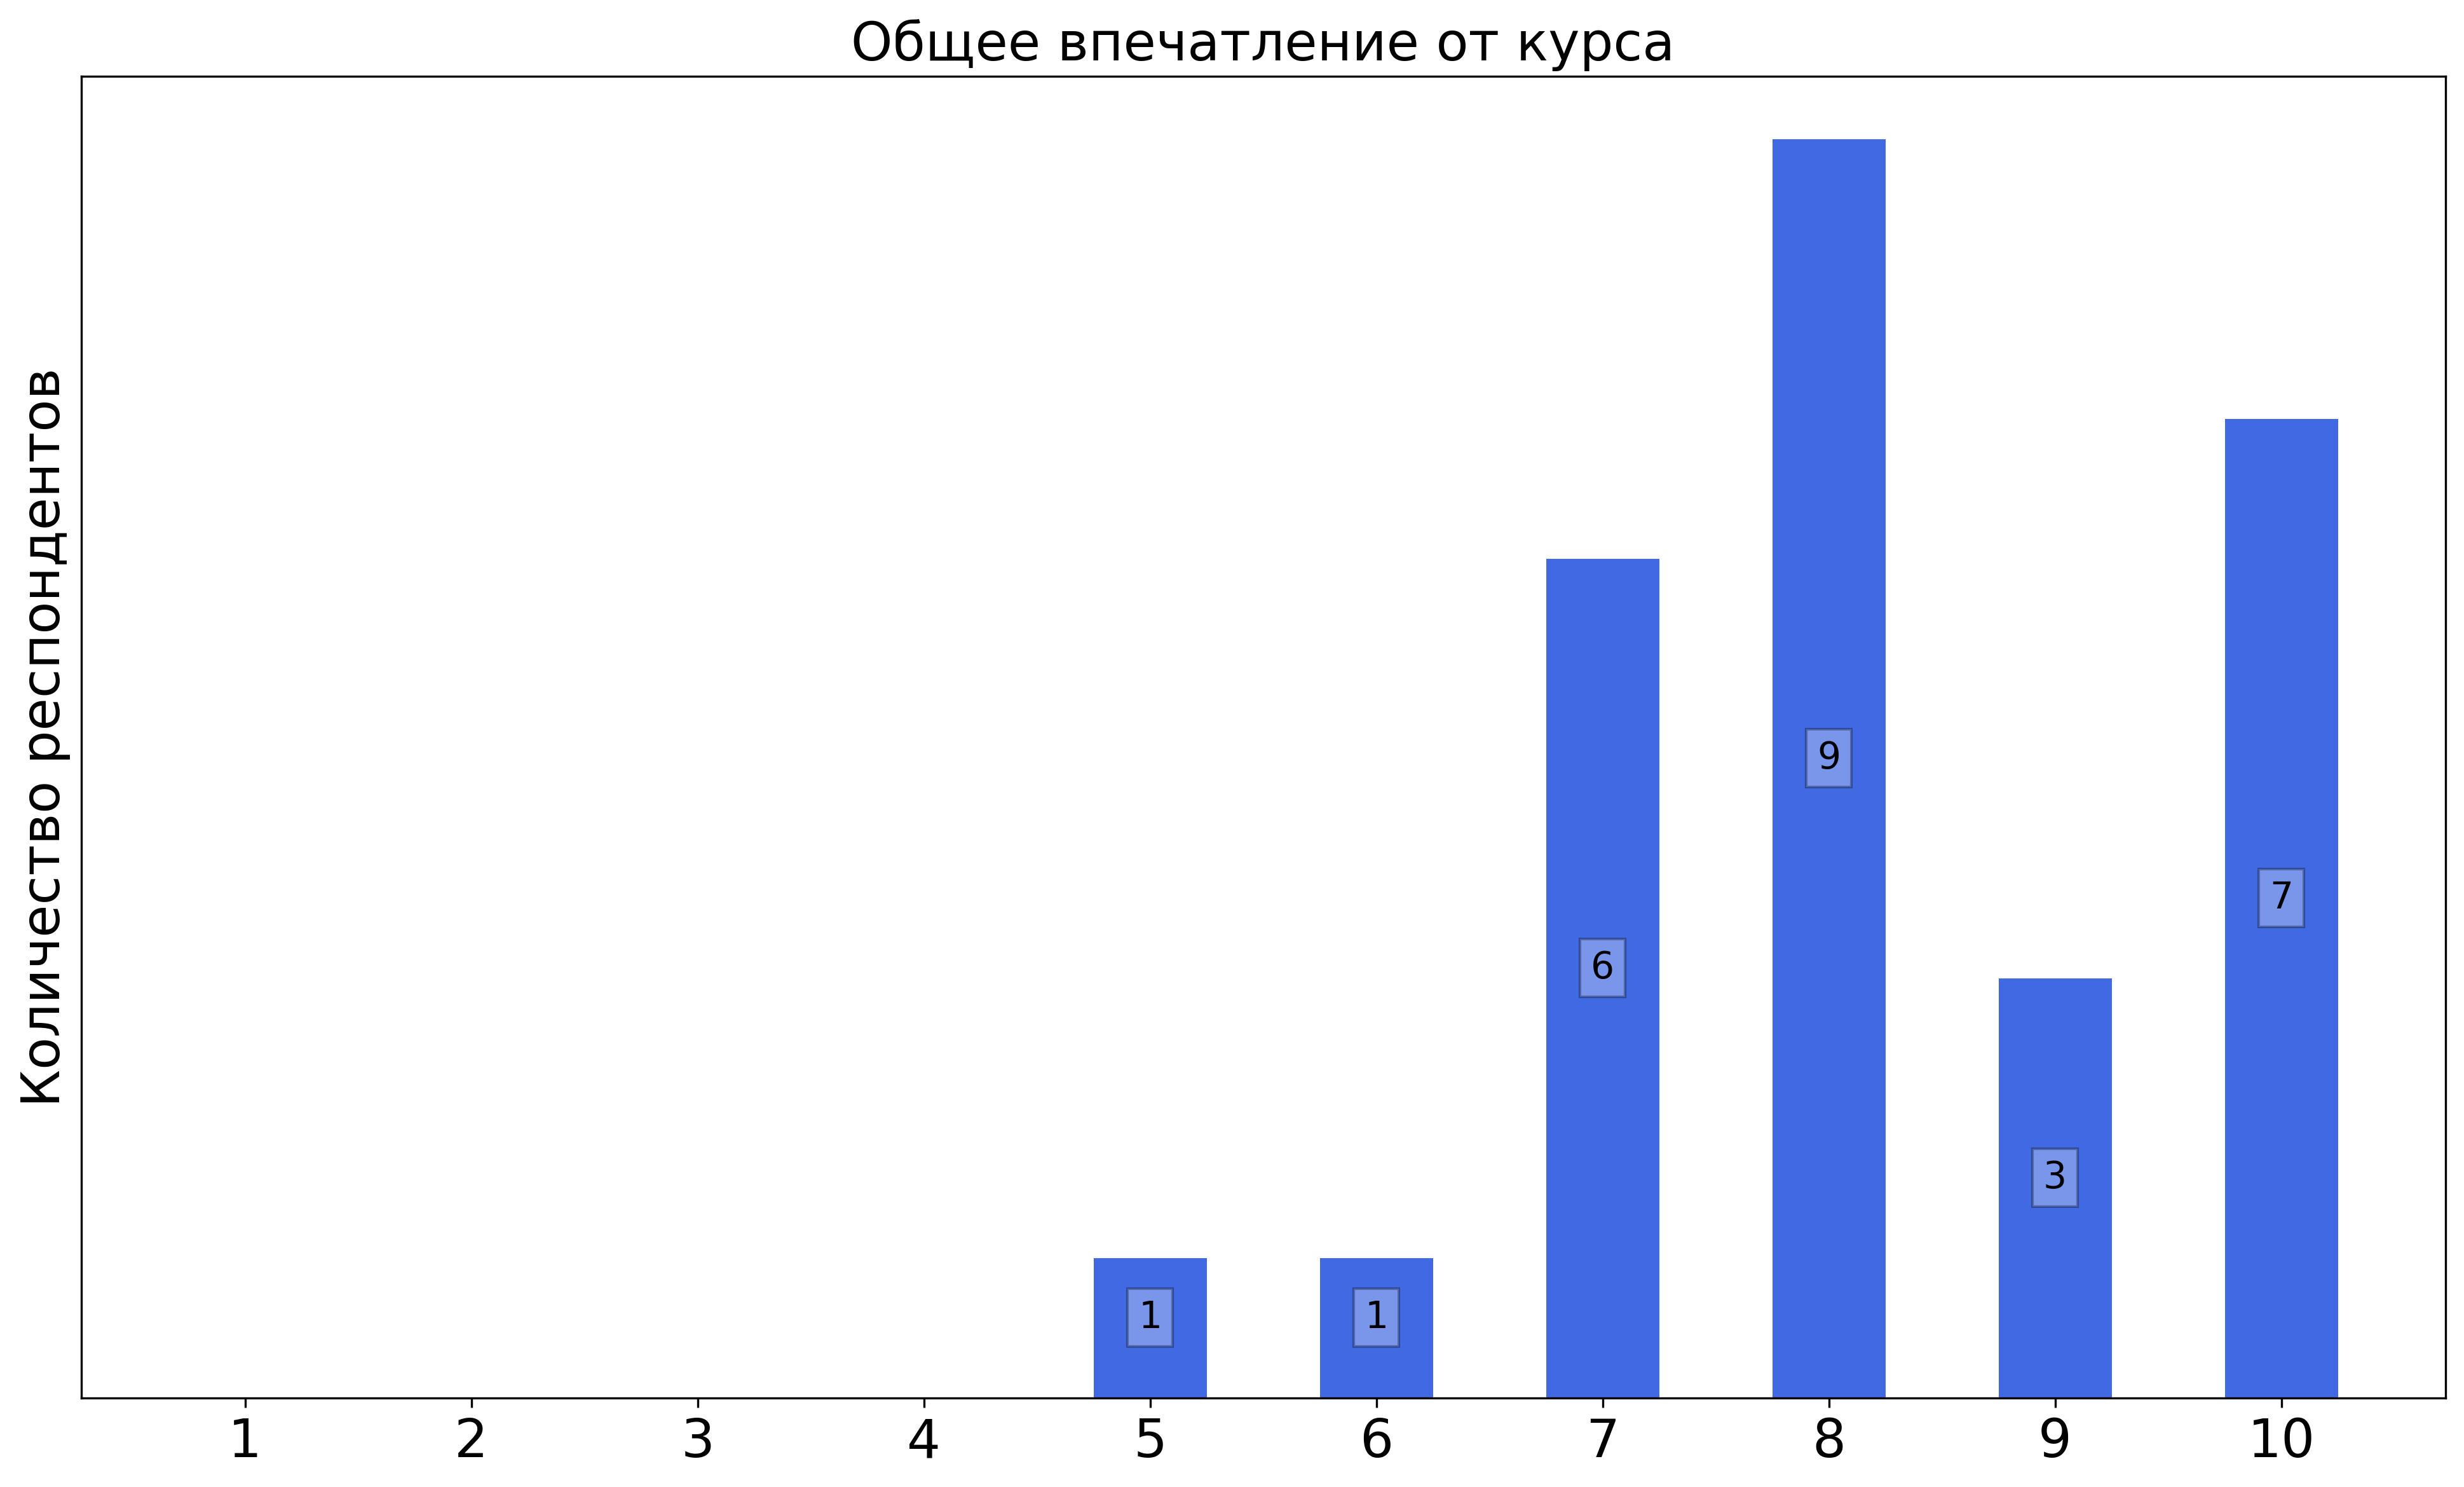
\includegraphics[width=\textwidth]{images/2 course/Кратные интегралы и теория поля/general-0.png}
			\end{subfigure}
			\begin{subfigure}[b]{0.45\textwidth}
				\centering
				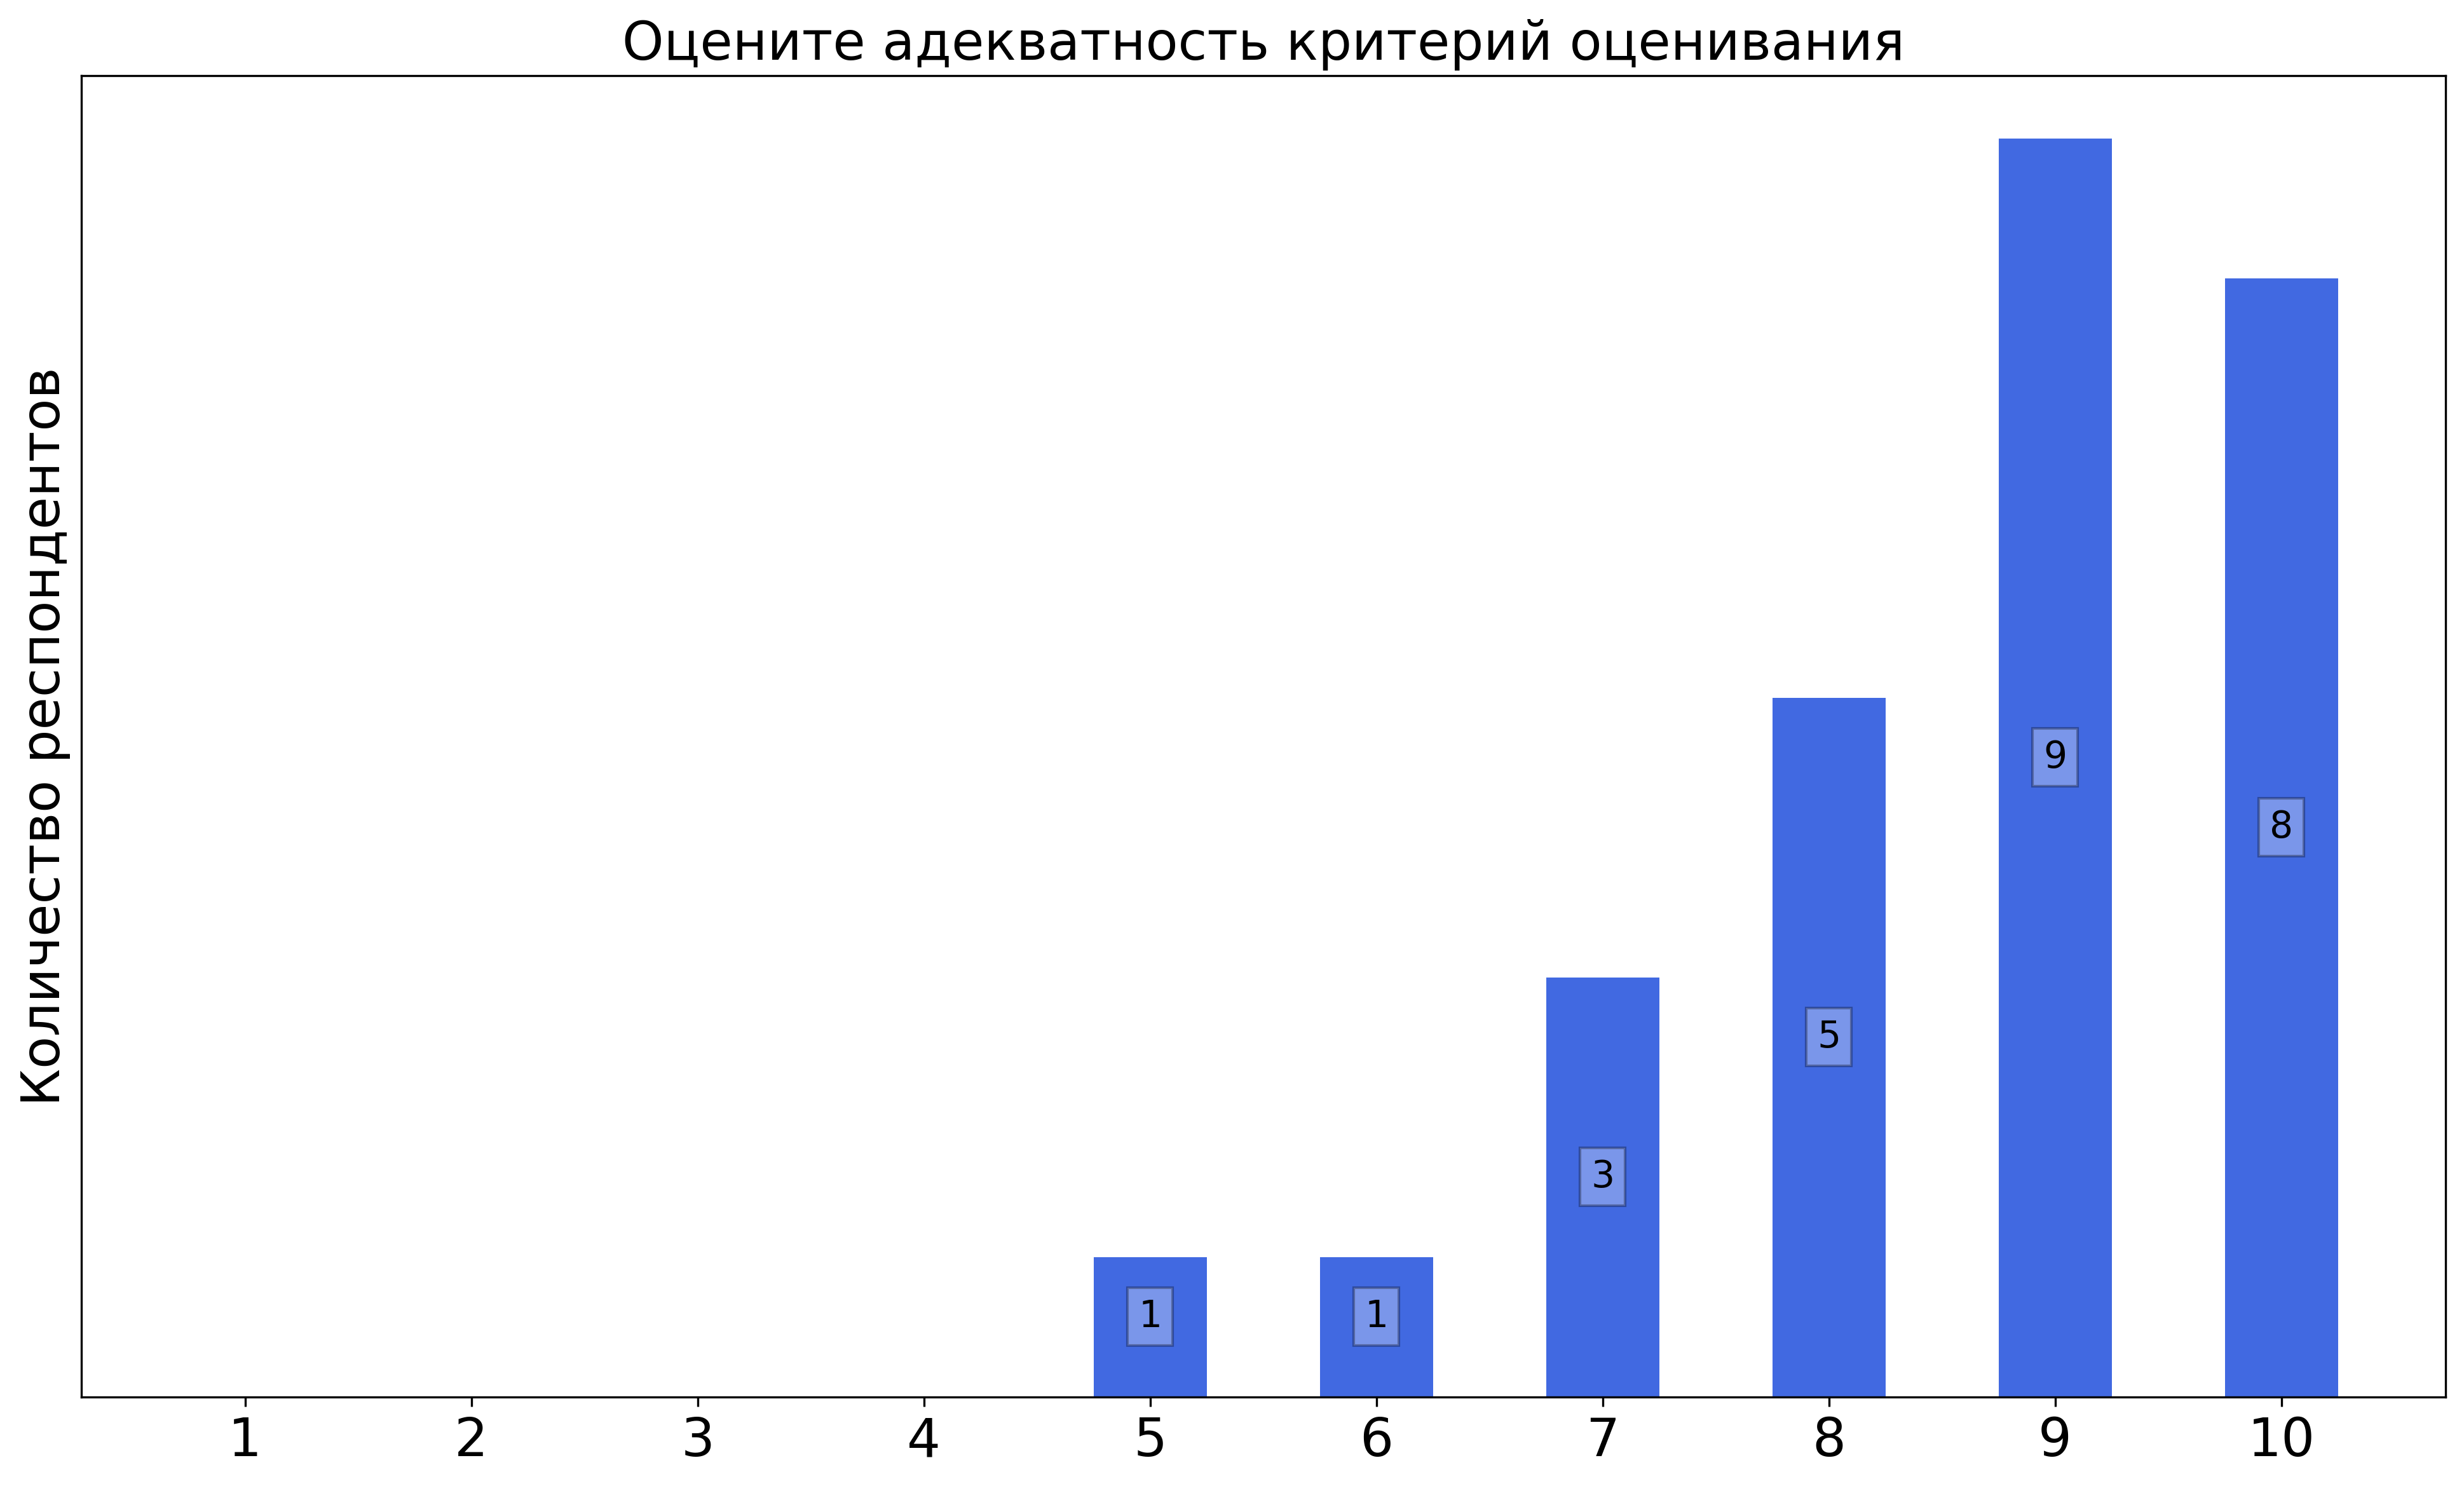
\includegraphics[width=\textwidth]{images/2 course/Кратные интегралы и теория поля/general-1.png}
			\end{subfigure}	
		\end{figure}

	\subsubsection{Материалы, использумые респондентами при изучении курса}

		\begin{figure}[H]
			\centering
			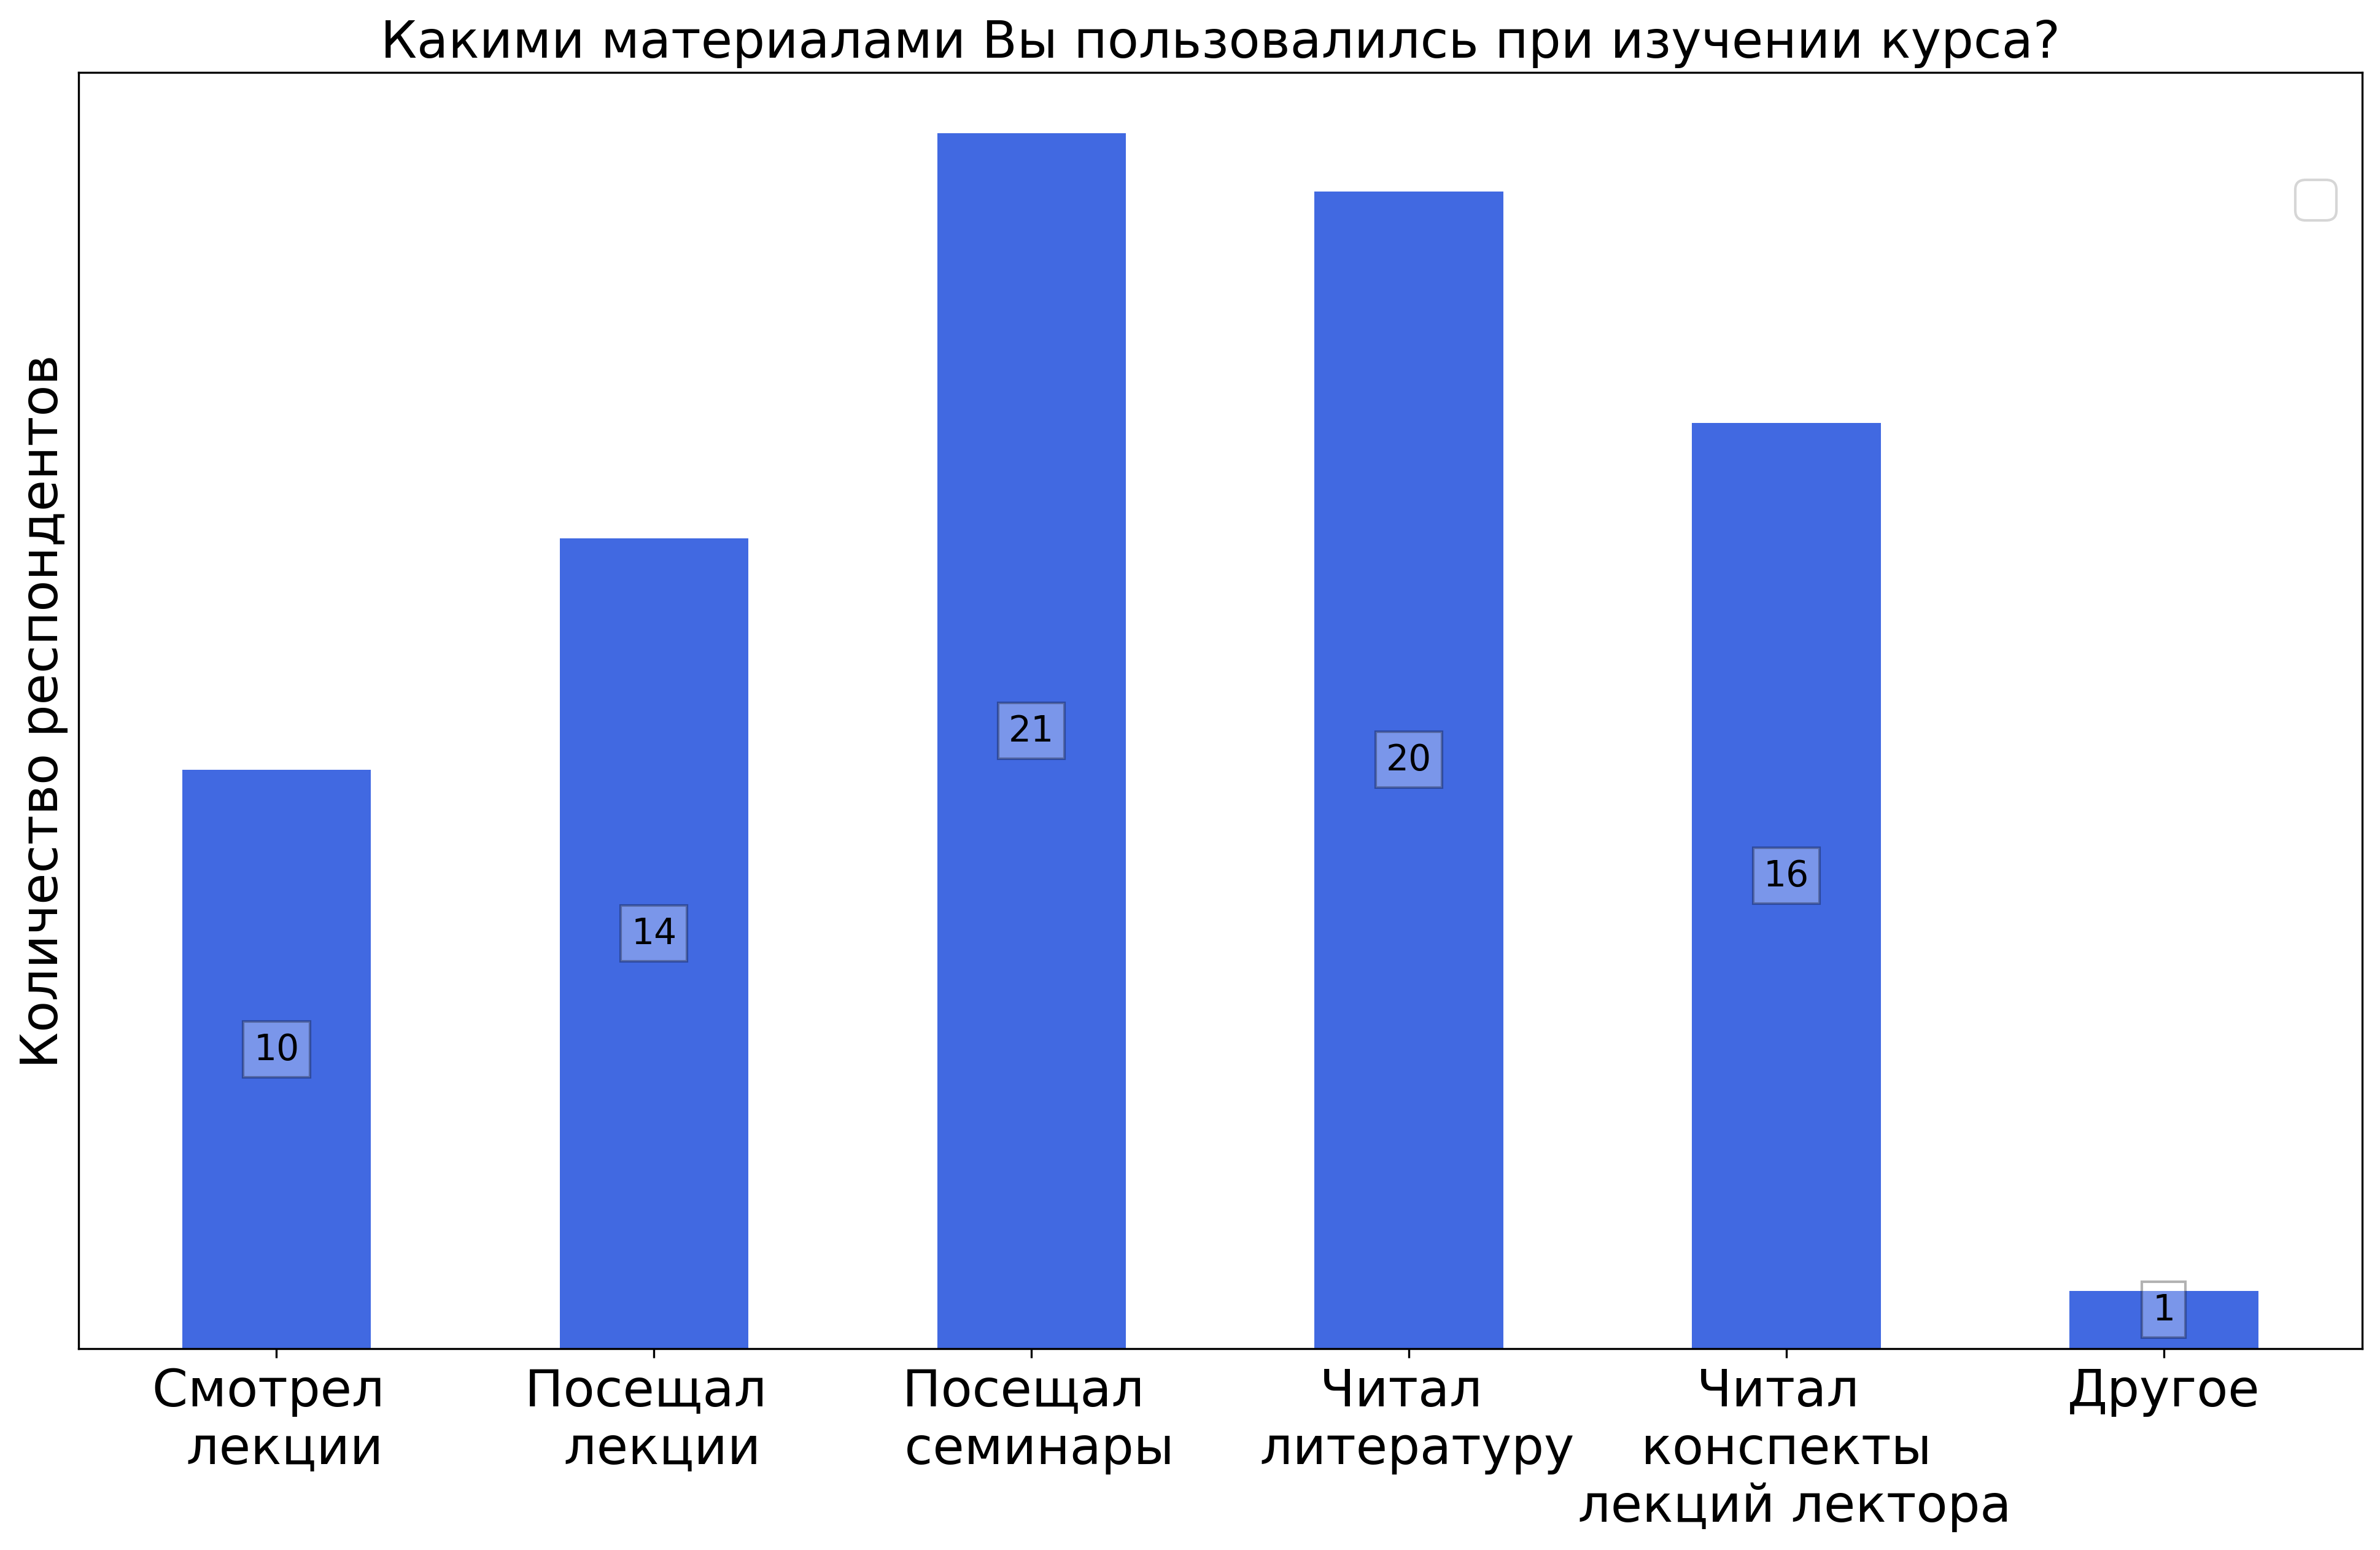
\includegraphics[width = 0.45\textwidth]{images/2 course/Кратные интегралы и теория поля/materials.png}
		\end{figure}

		\textit{В качестве других источников информации студенты указали:} 
		\begin{itemize}
            \item записи семинаров других преподавателей.
		\end{itemize}

	\subsubsection{Отзыв студентов о лекциях. Лектор: Петрович А.Ю.}

		\begin{figure}[H]
			\centering
            \begin{subfigure}[b]{0.45\textwidth}
				\centering
				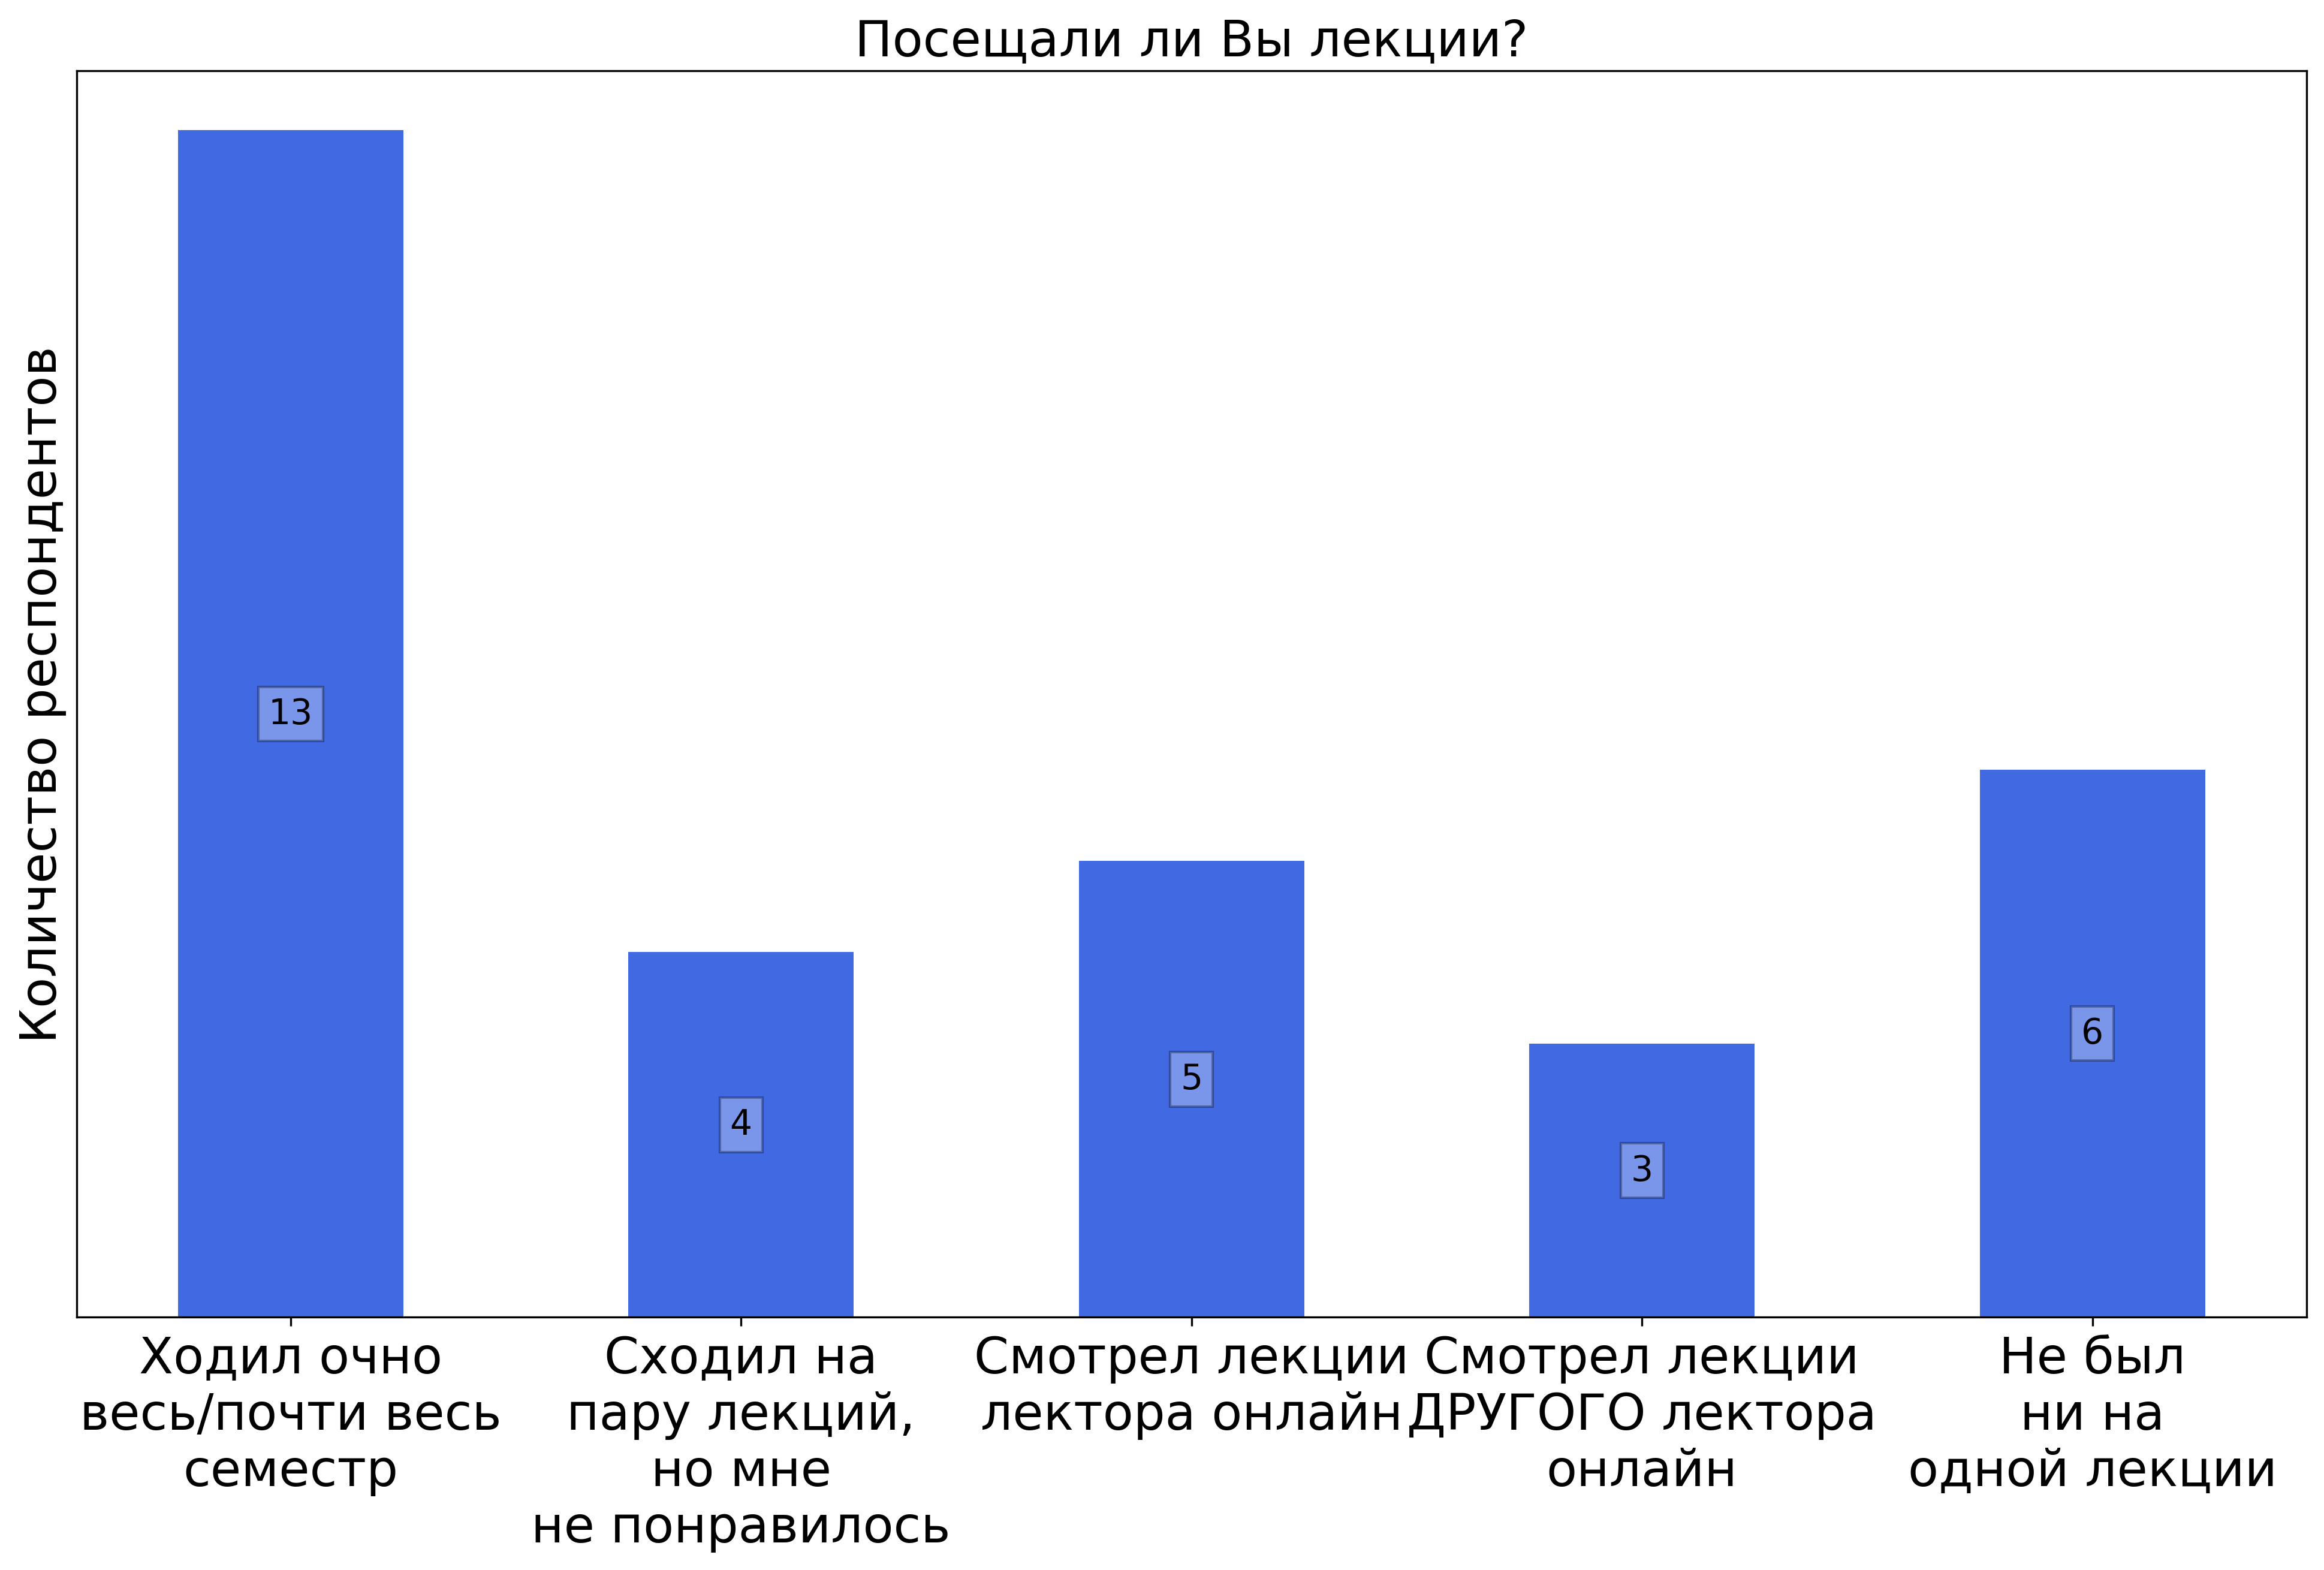
\includegraphics[width=\textwidth]{images/2 course/Кратные интегралы и теория поля/lecturer-questions-Петрович А.Ю.-0.png}
			\end{subfigure}
			\begin{subfigure}[b]{0.45\textwidth}
				\centering
				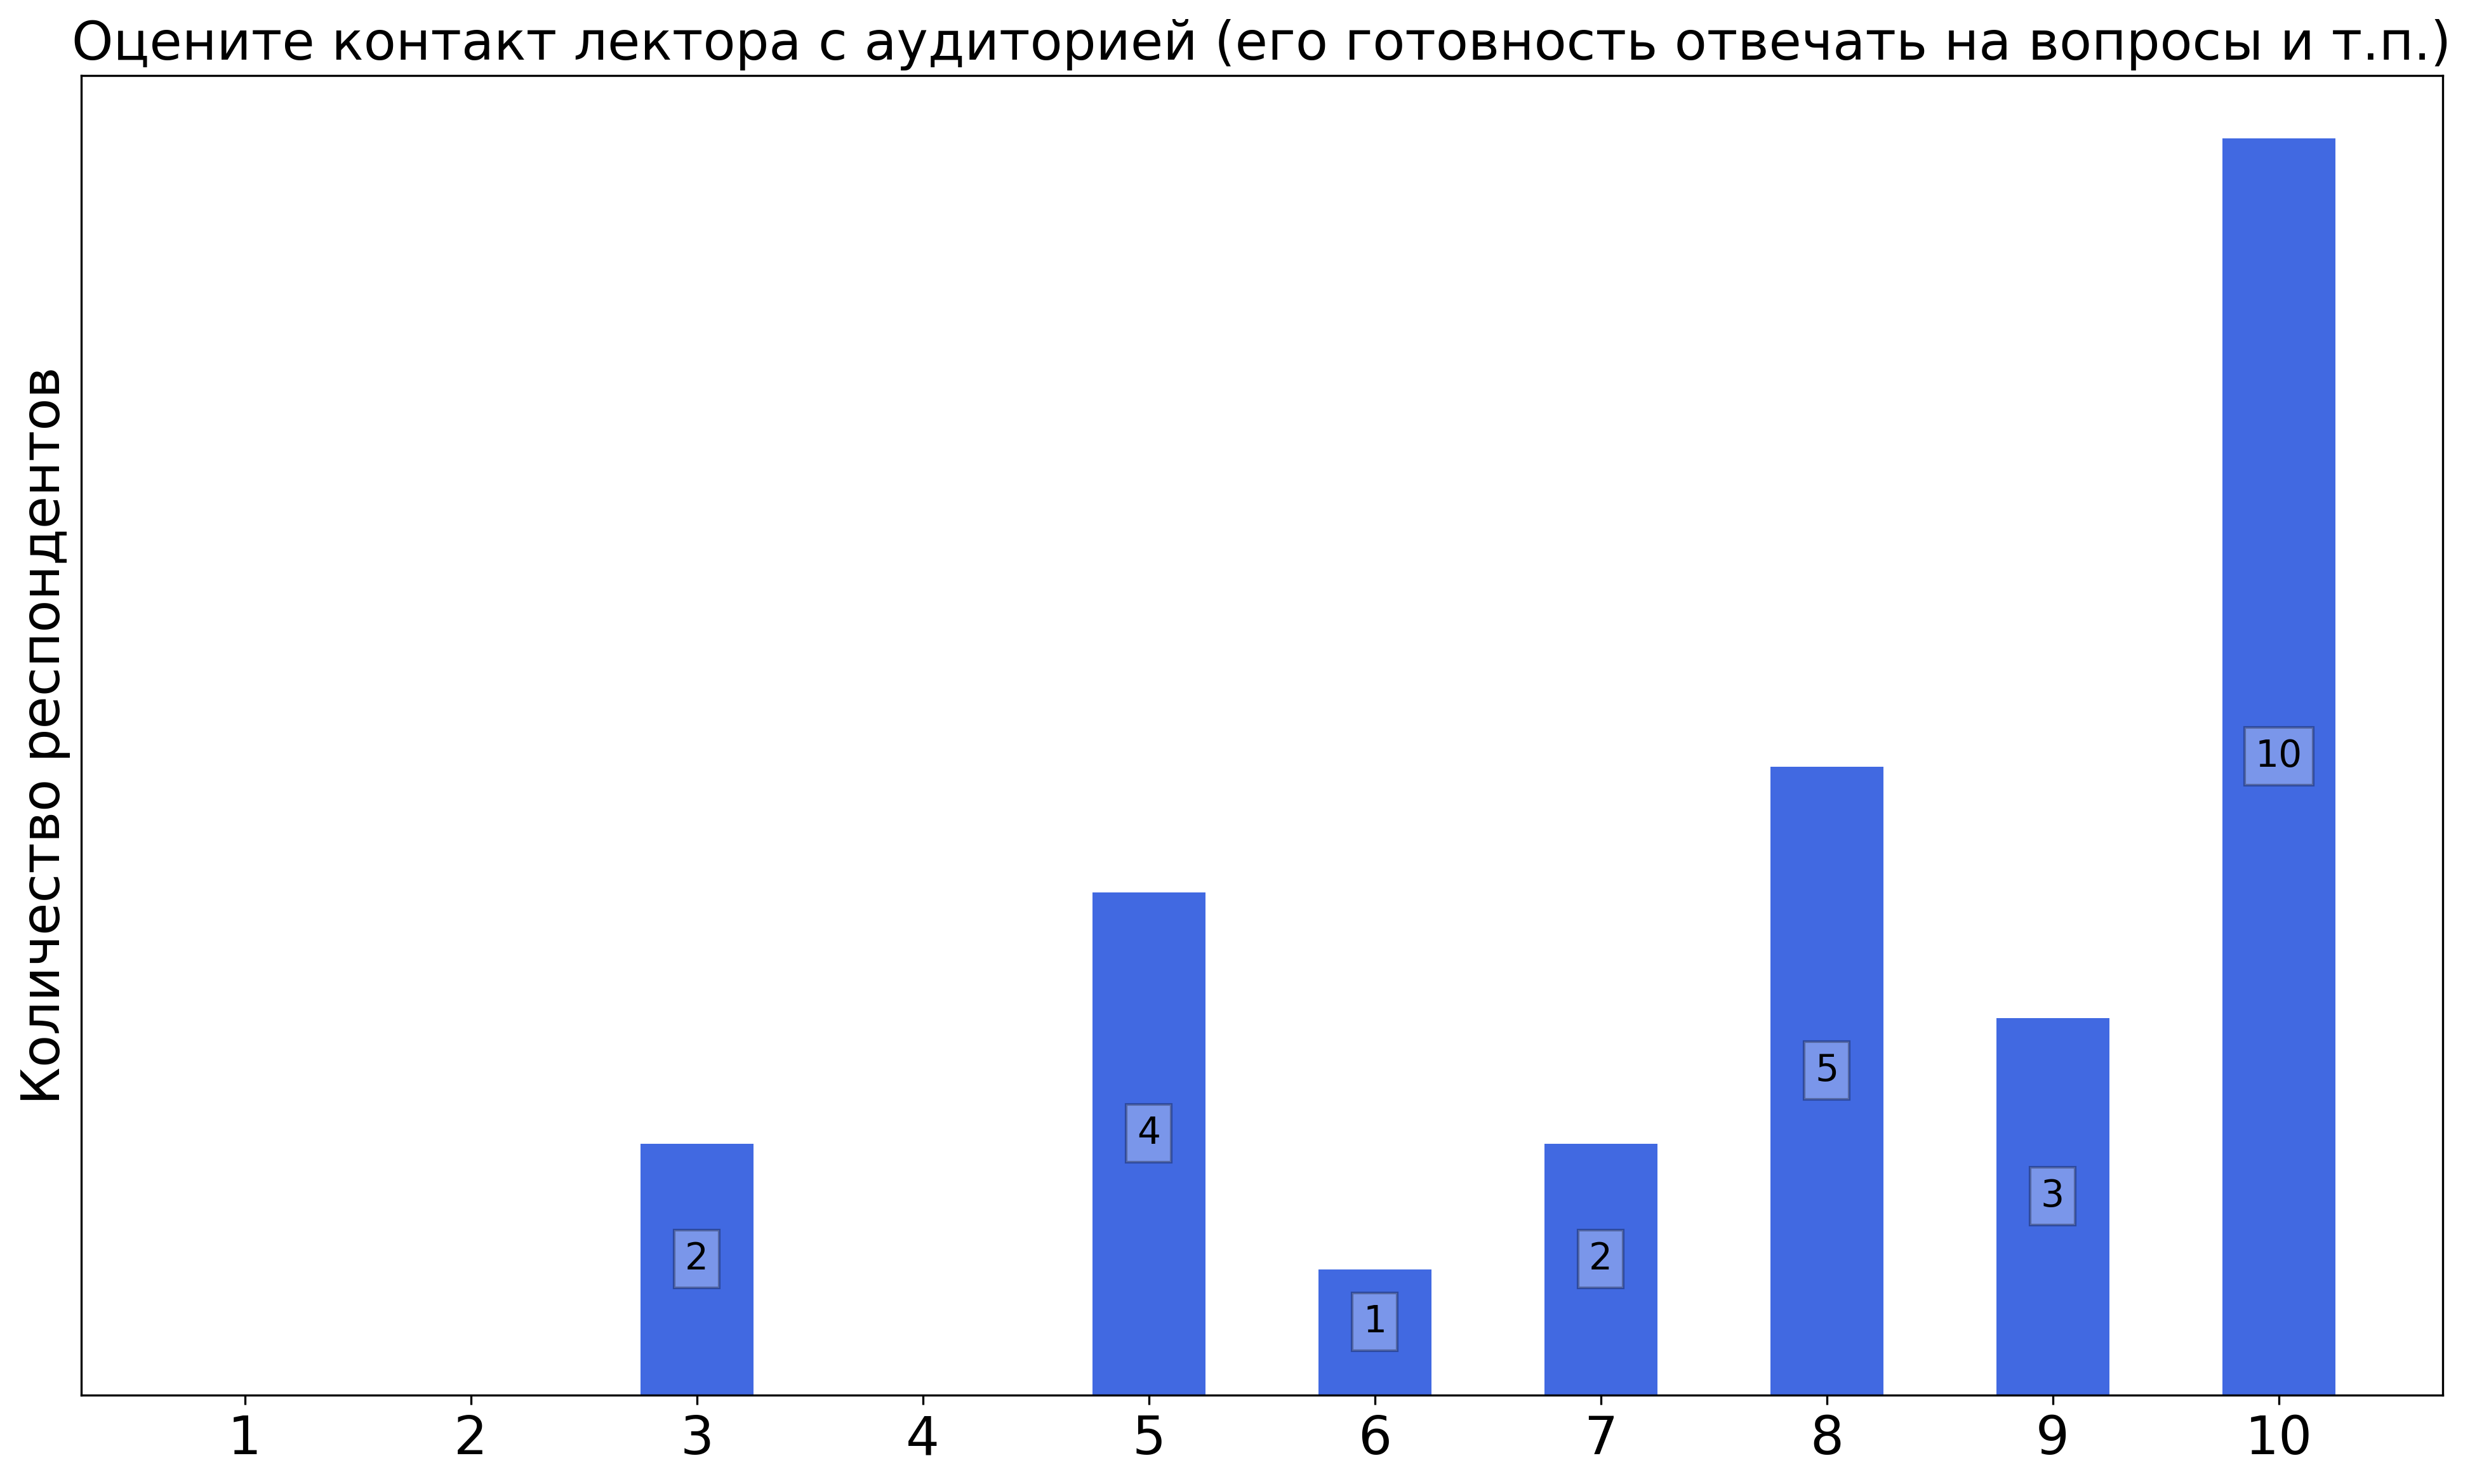
\includegraphics[width=\textwidth]{images/2 course/Кратные интегралы и теория поля/lecturer-marks-Петрович А.Ю.-0.png}
			\end{subfigure}
			\begin{subfigure}[b]{0.45\textwidth}
				\centering
				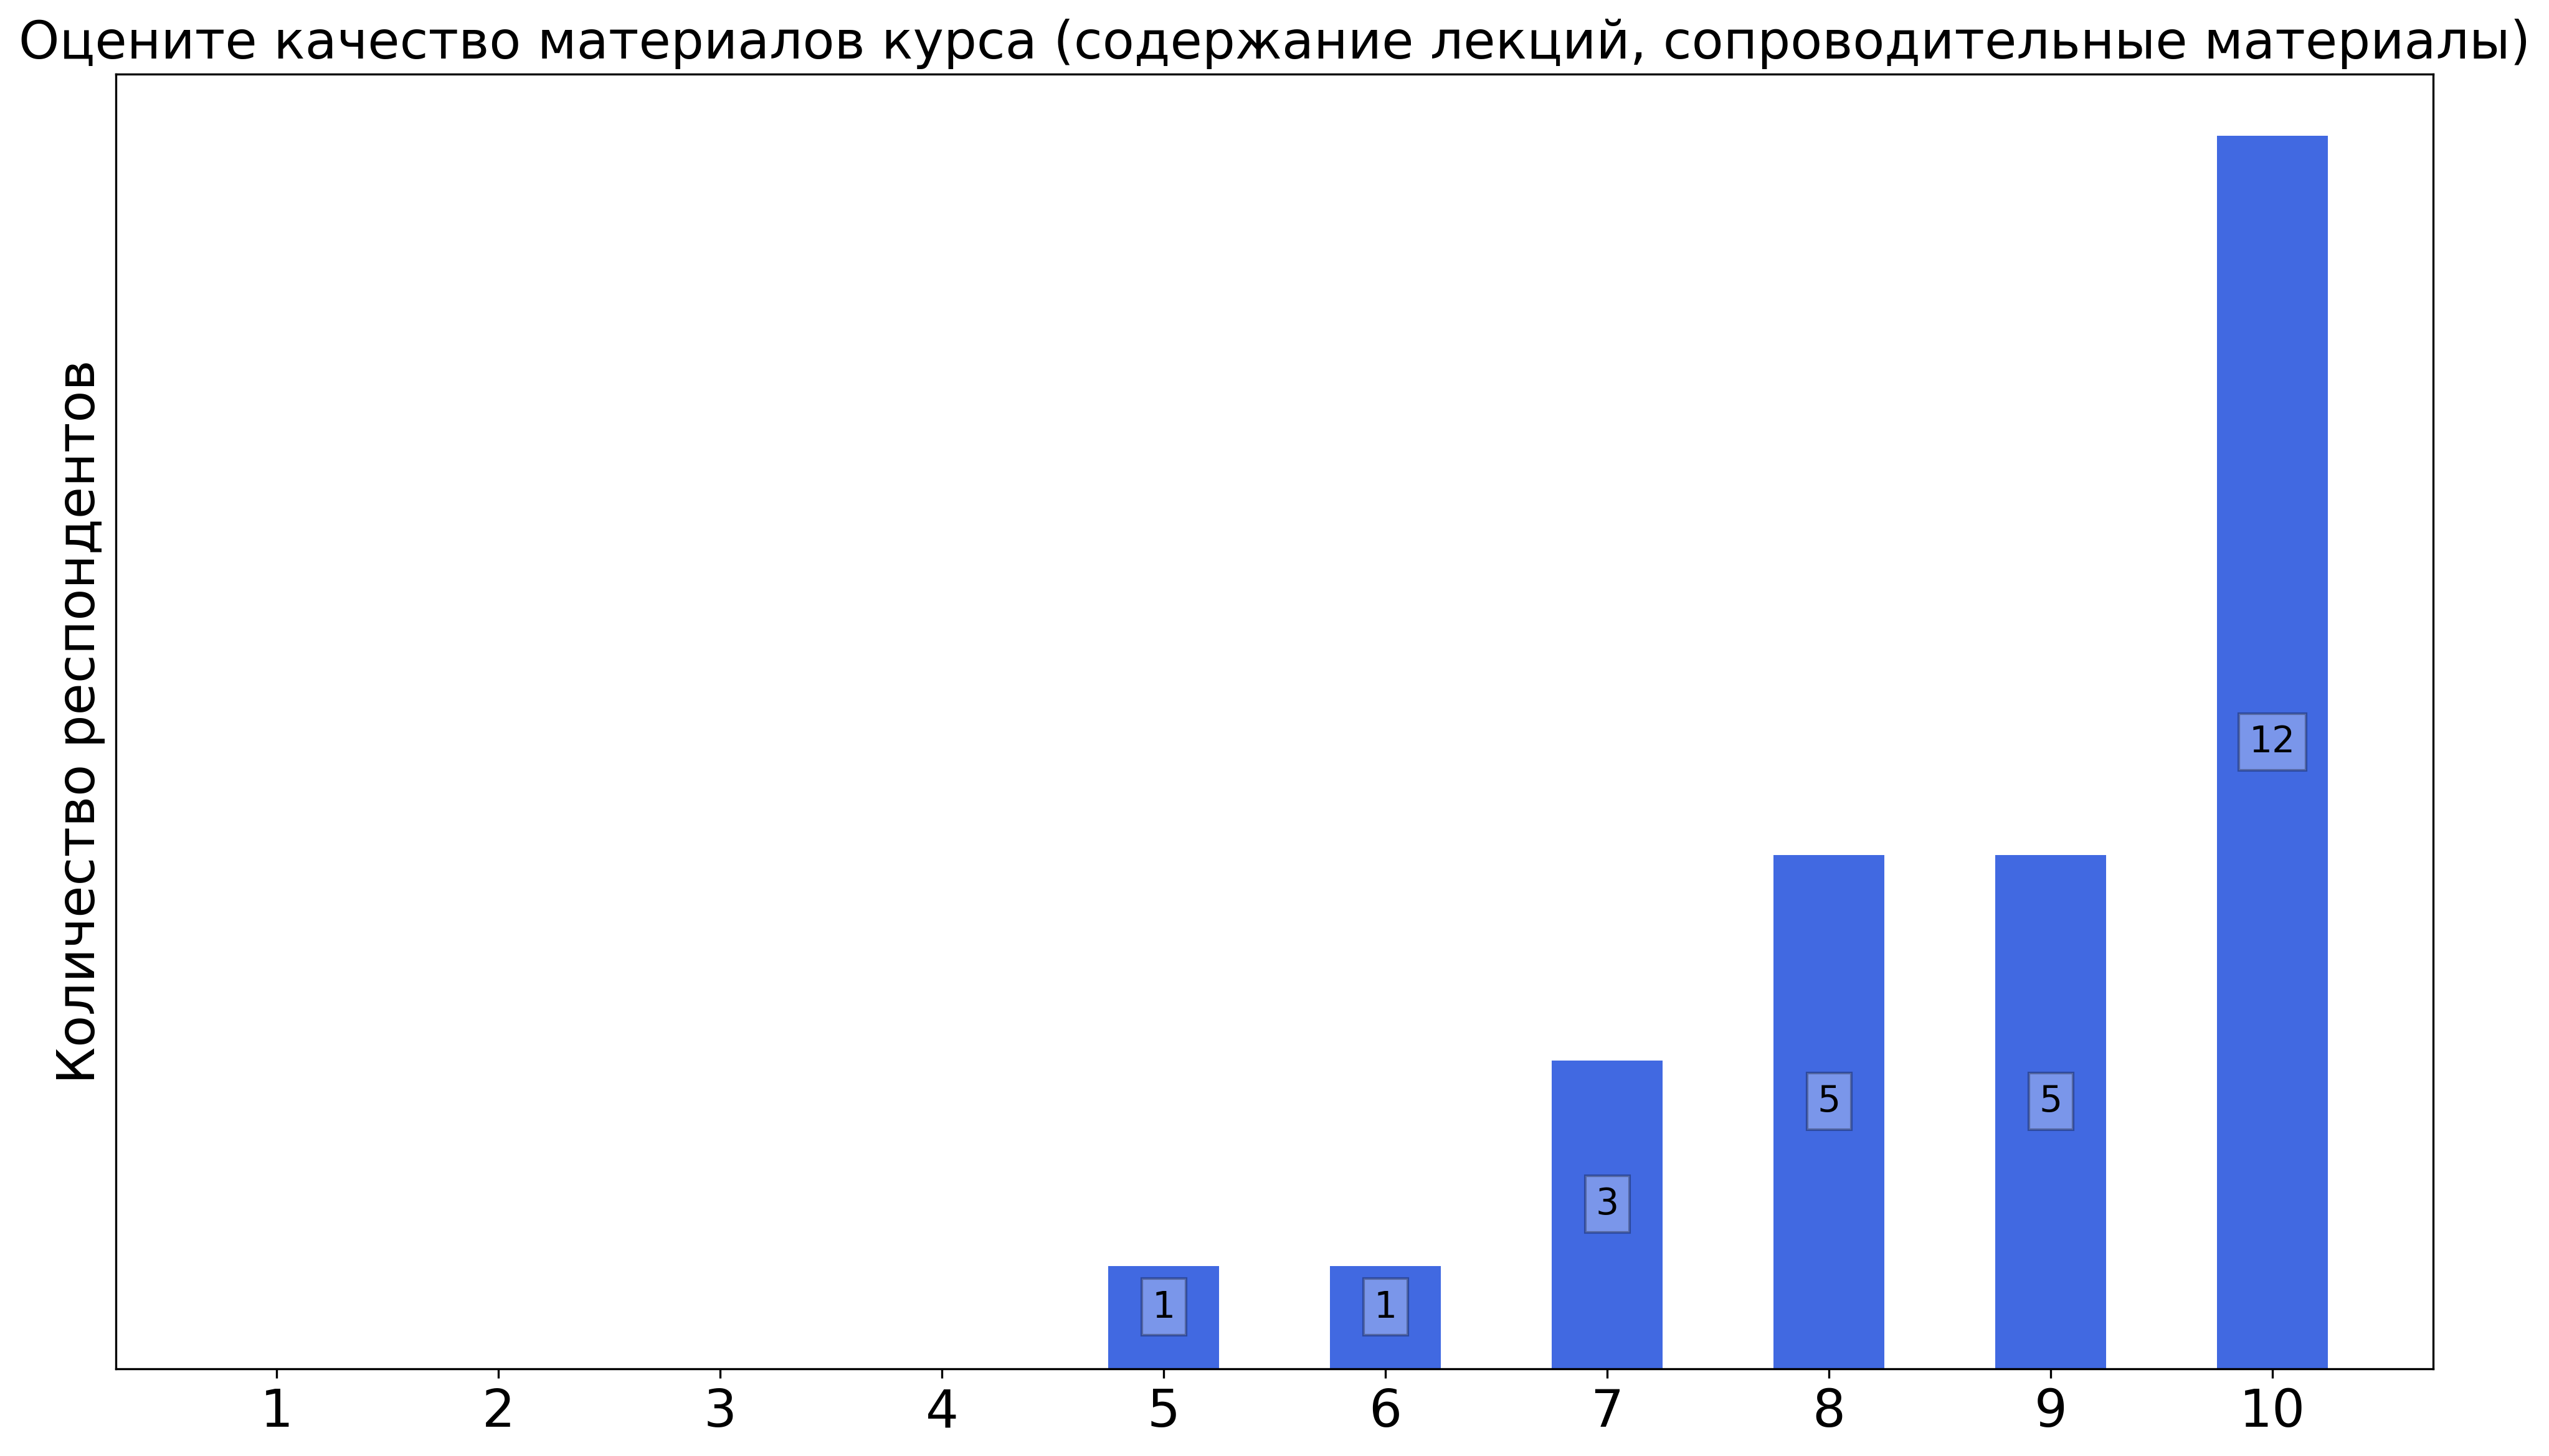
\includegraphics[width=\textwidth]{images/2 course/Кратные интегралы и теория поля/lecturer-marks-Петрович А.Ю.-1.png}
			\end{subfigure}
			\begin{subfigure}[b]{0.45\textwidth}
				\centering
				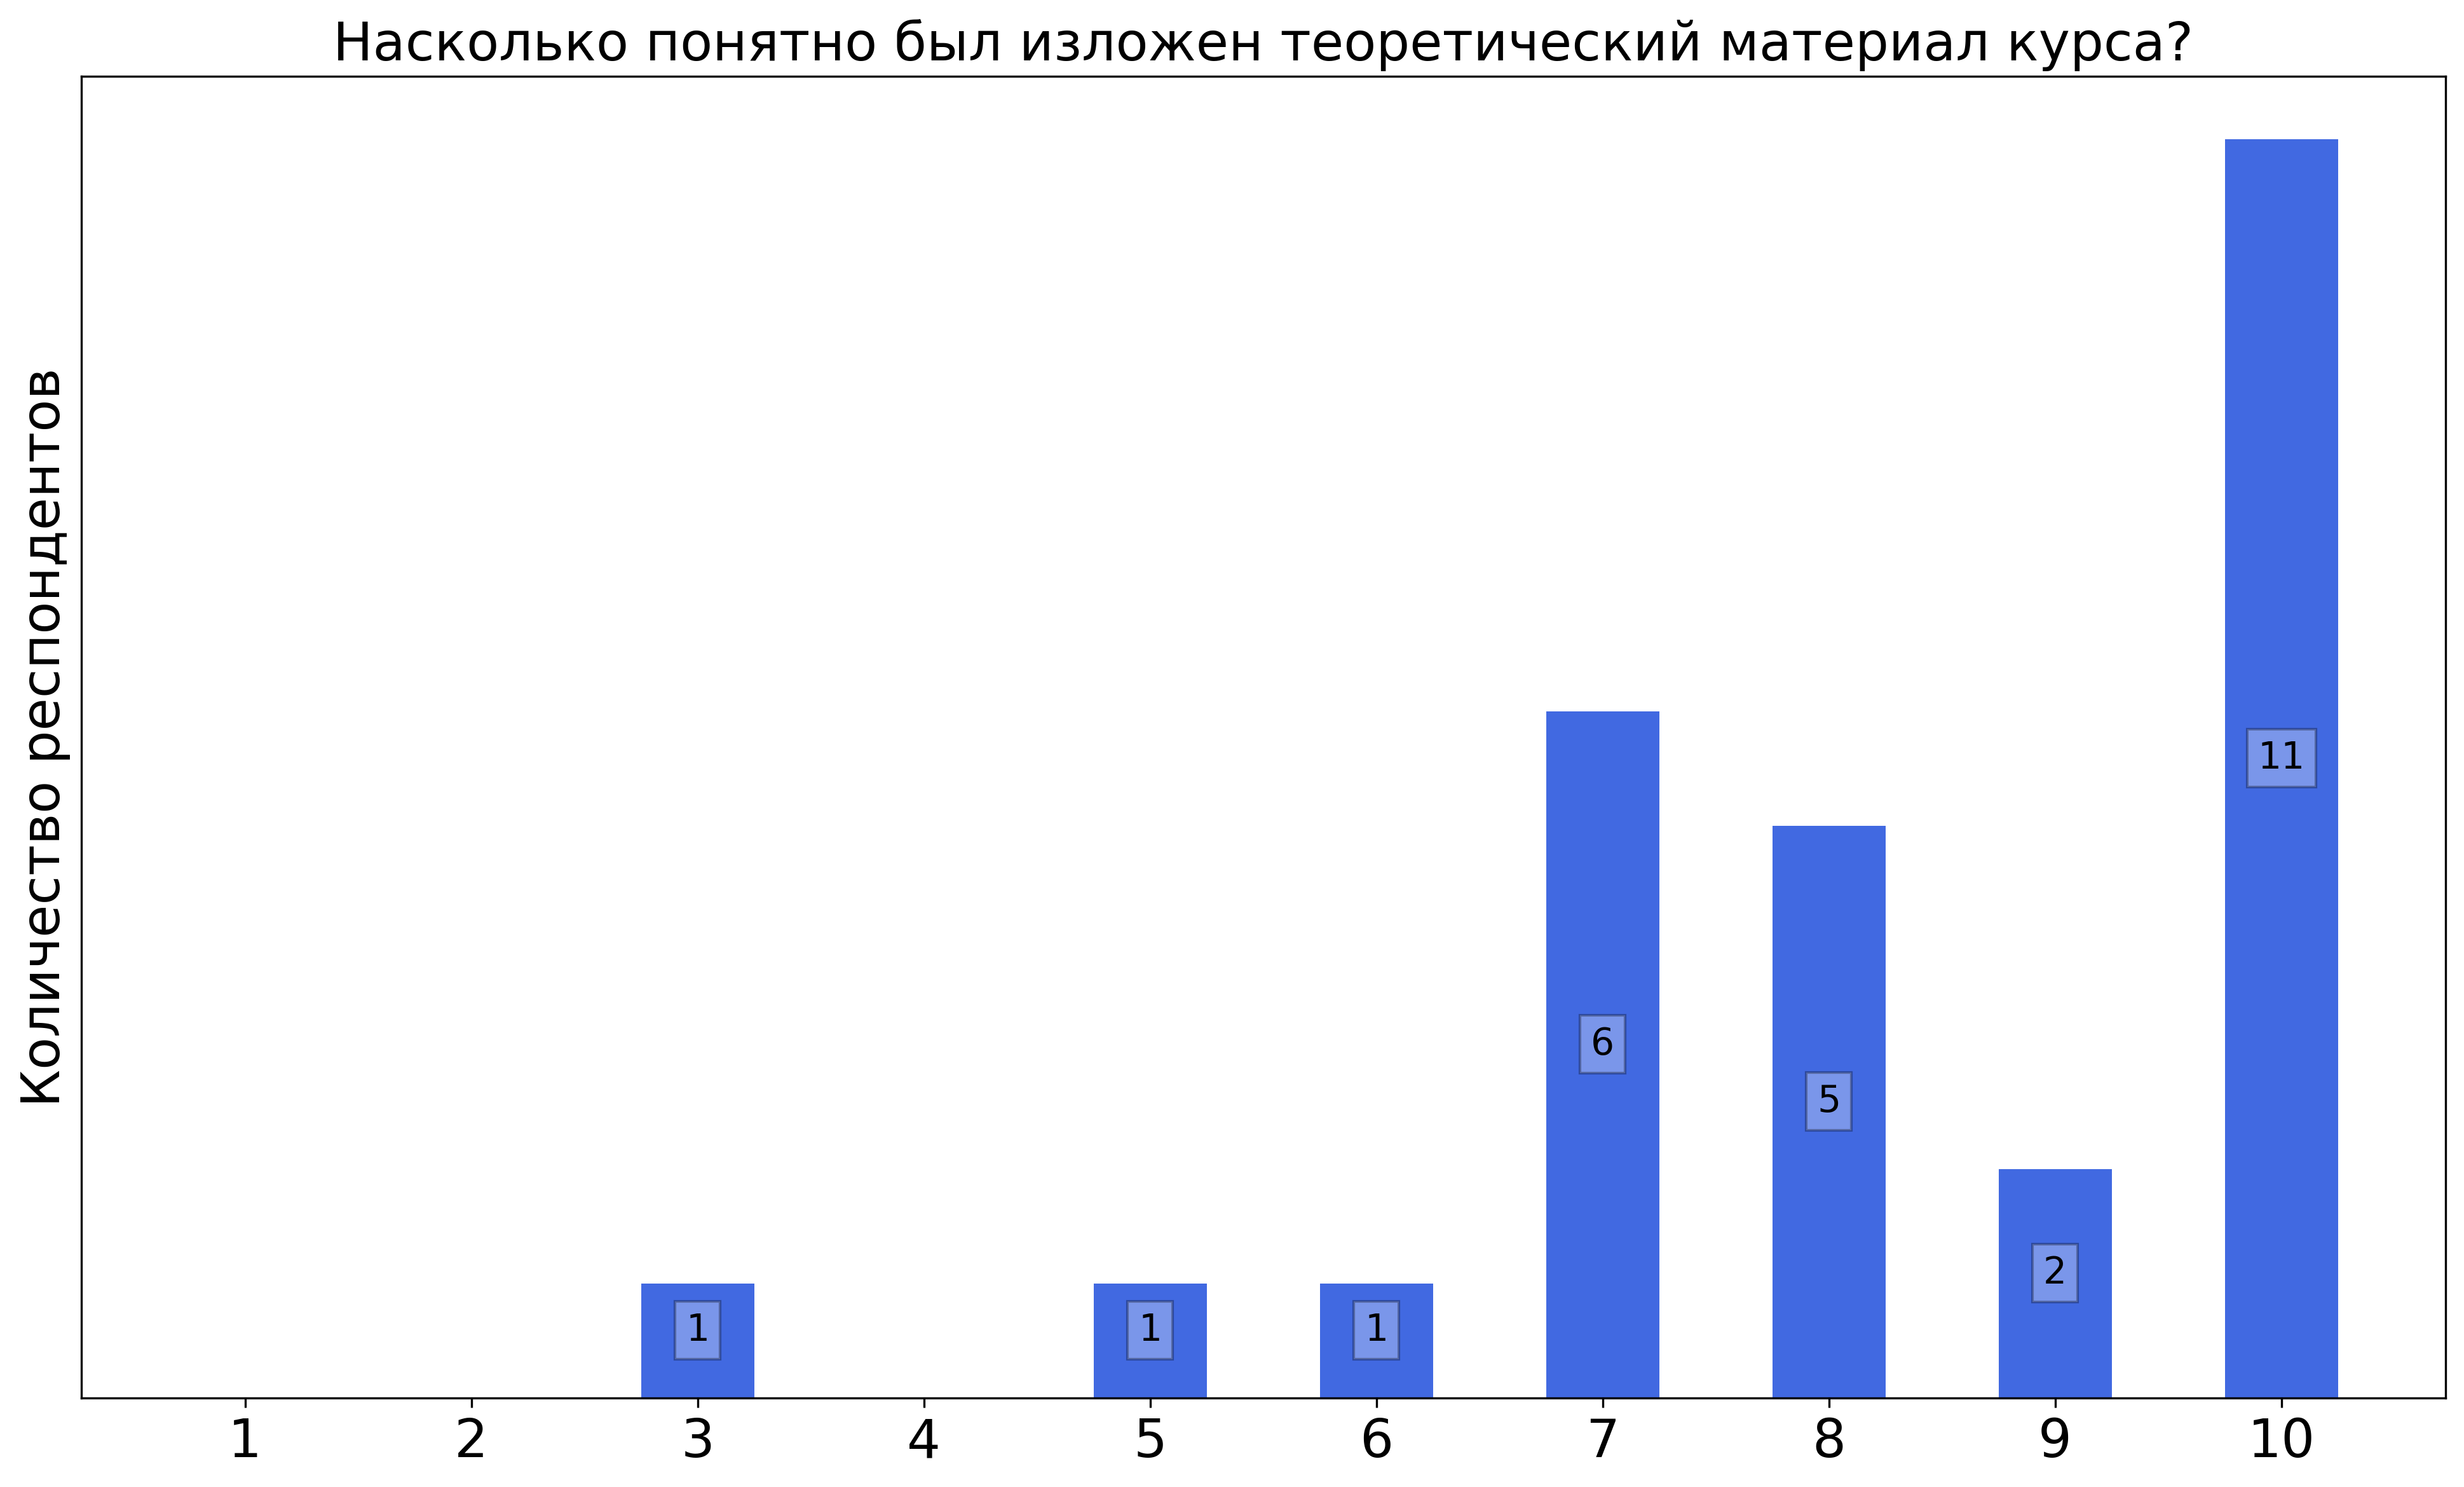
\includegraphics[width=\textwidth]{images/2 course/Кратные интегралы и теория поля/lecturer-marks-Петрович А.Ю.-2.png}
			\end{subfigure}	
			\begin{subfigure}[b]{0.45\textwidth}
				\centering
				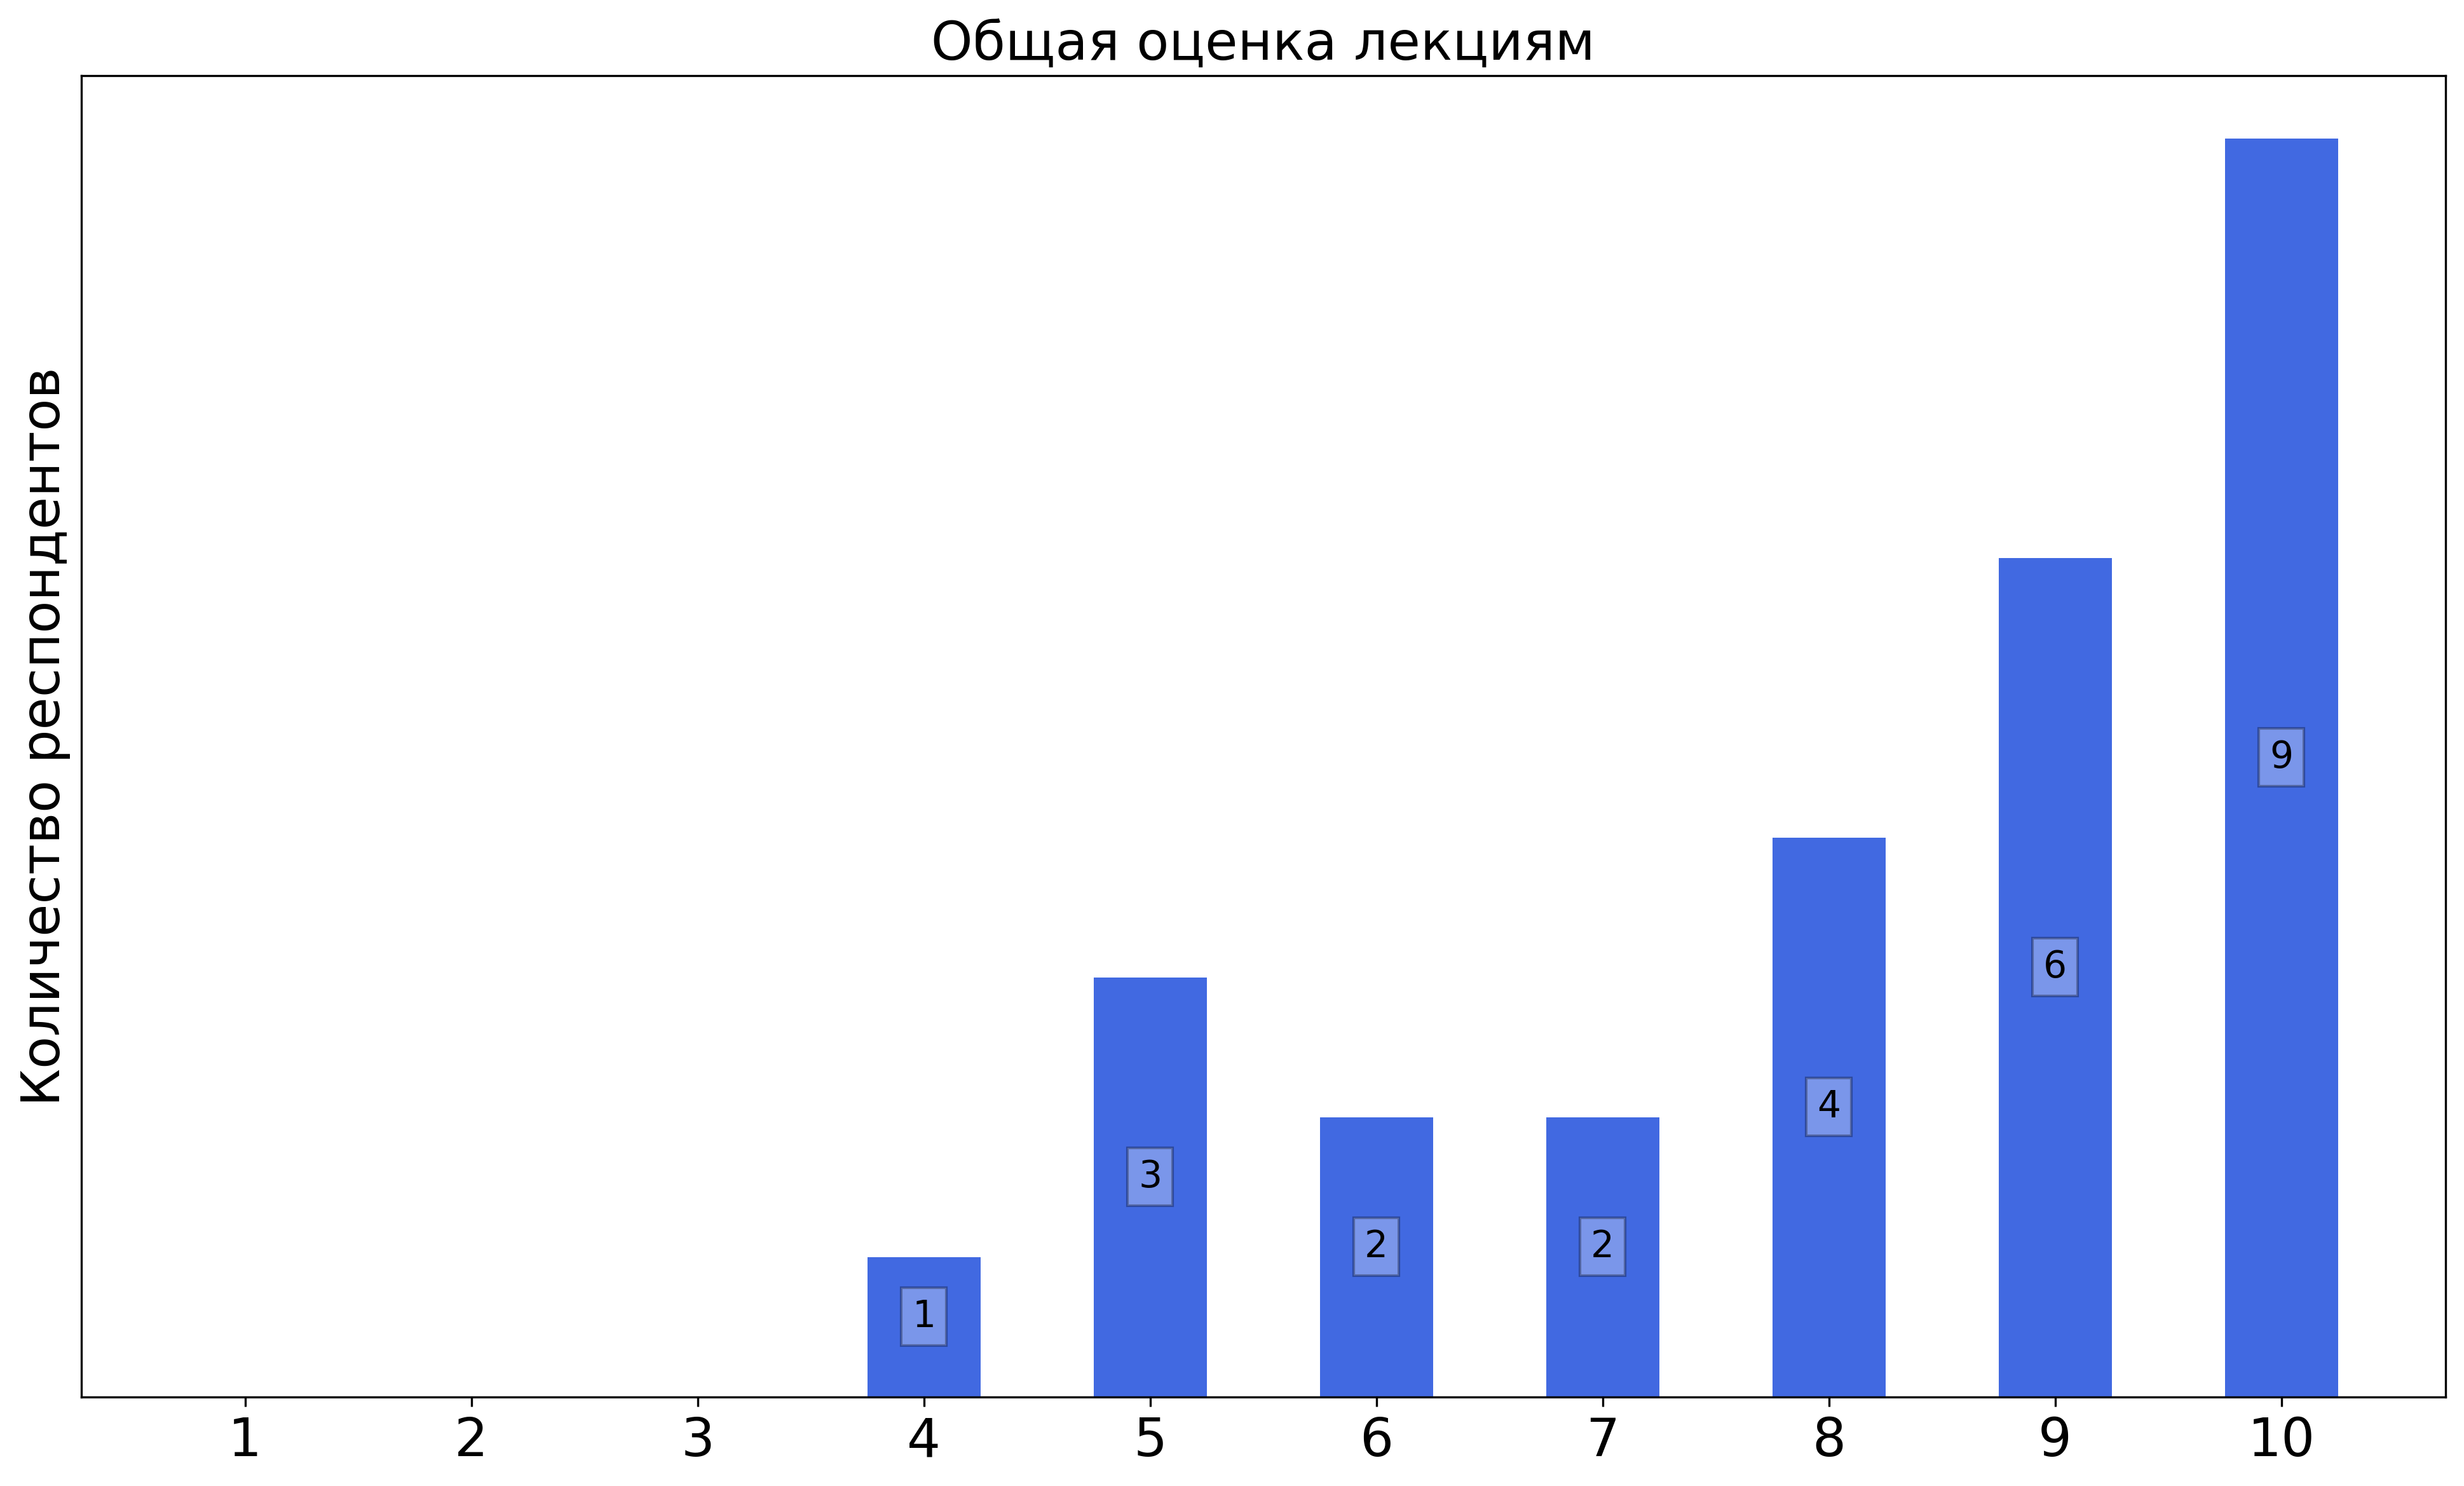
\includegraphics[width=\textwidth]{images/2 course/Кратные интегралы и теория поля/lecturer-marks-Петрович А.Ю.-3.png}
			\end{subfigure}
			\caption{Оценки респондентов о качестве преподавания лекций по курсу <<Кратные интегралы и теория поля>>}
		\end{figure}

		\textbf{Комментарии студентов о лекциях\protect\footnote{сохранены оригинальные орфография и пунктуация}}
            \begin{commentbox} 
                А.Ю. Петрович - очень хороший преподаватель и лектор, но зачастую тяжело успевать за ним записывать, а уж тем более понимать доказательства объемных и идейно сложных теорем 
                Однако его книга написана простым и понятным языком, а изложение лекций во многом основано на книге 
            \end{commentbox} 
        
            \begin{commentbox} 
                Преподаватель быстро рассказывает и не совсем разборчиво пишет, из-за чего тяжело держать нить повествования 
            \end{commentbox} 
    
    
    \subsubsection{Отзыв студентов о семинарах. Семинарист: Барабанщиков А.В.}
		\begin{figure}[H]
			\centering
			\begin{subfigure}[b]{0.45\textwidth}
				\centering
				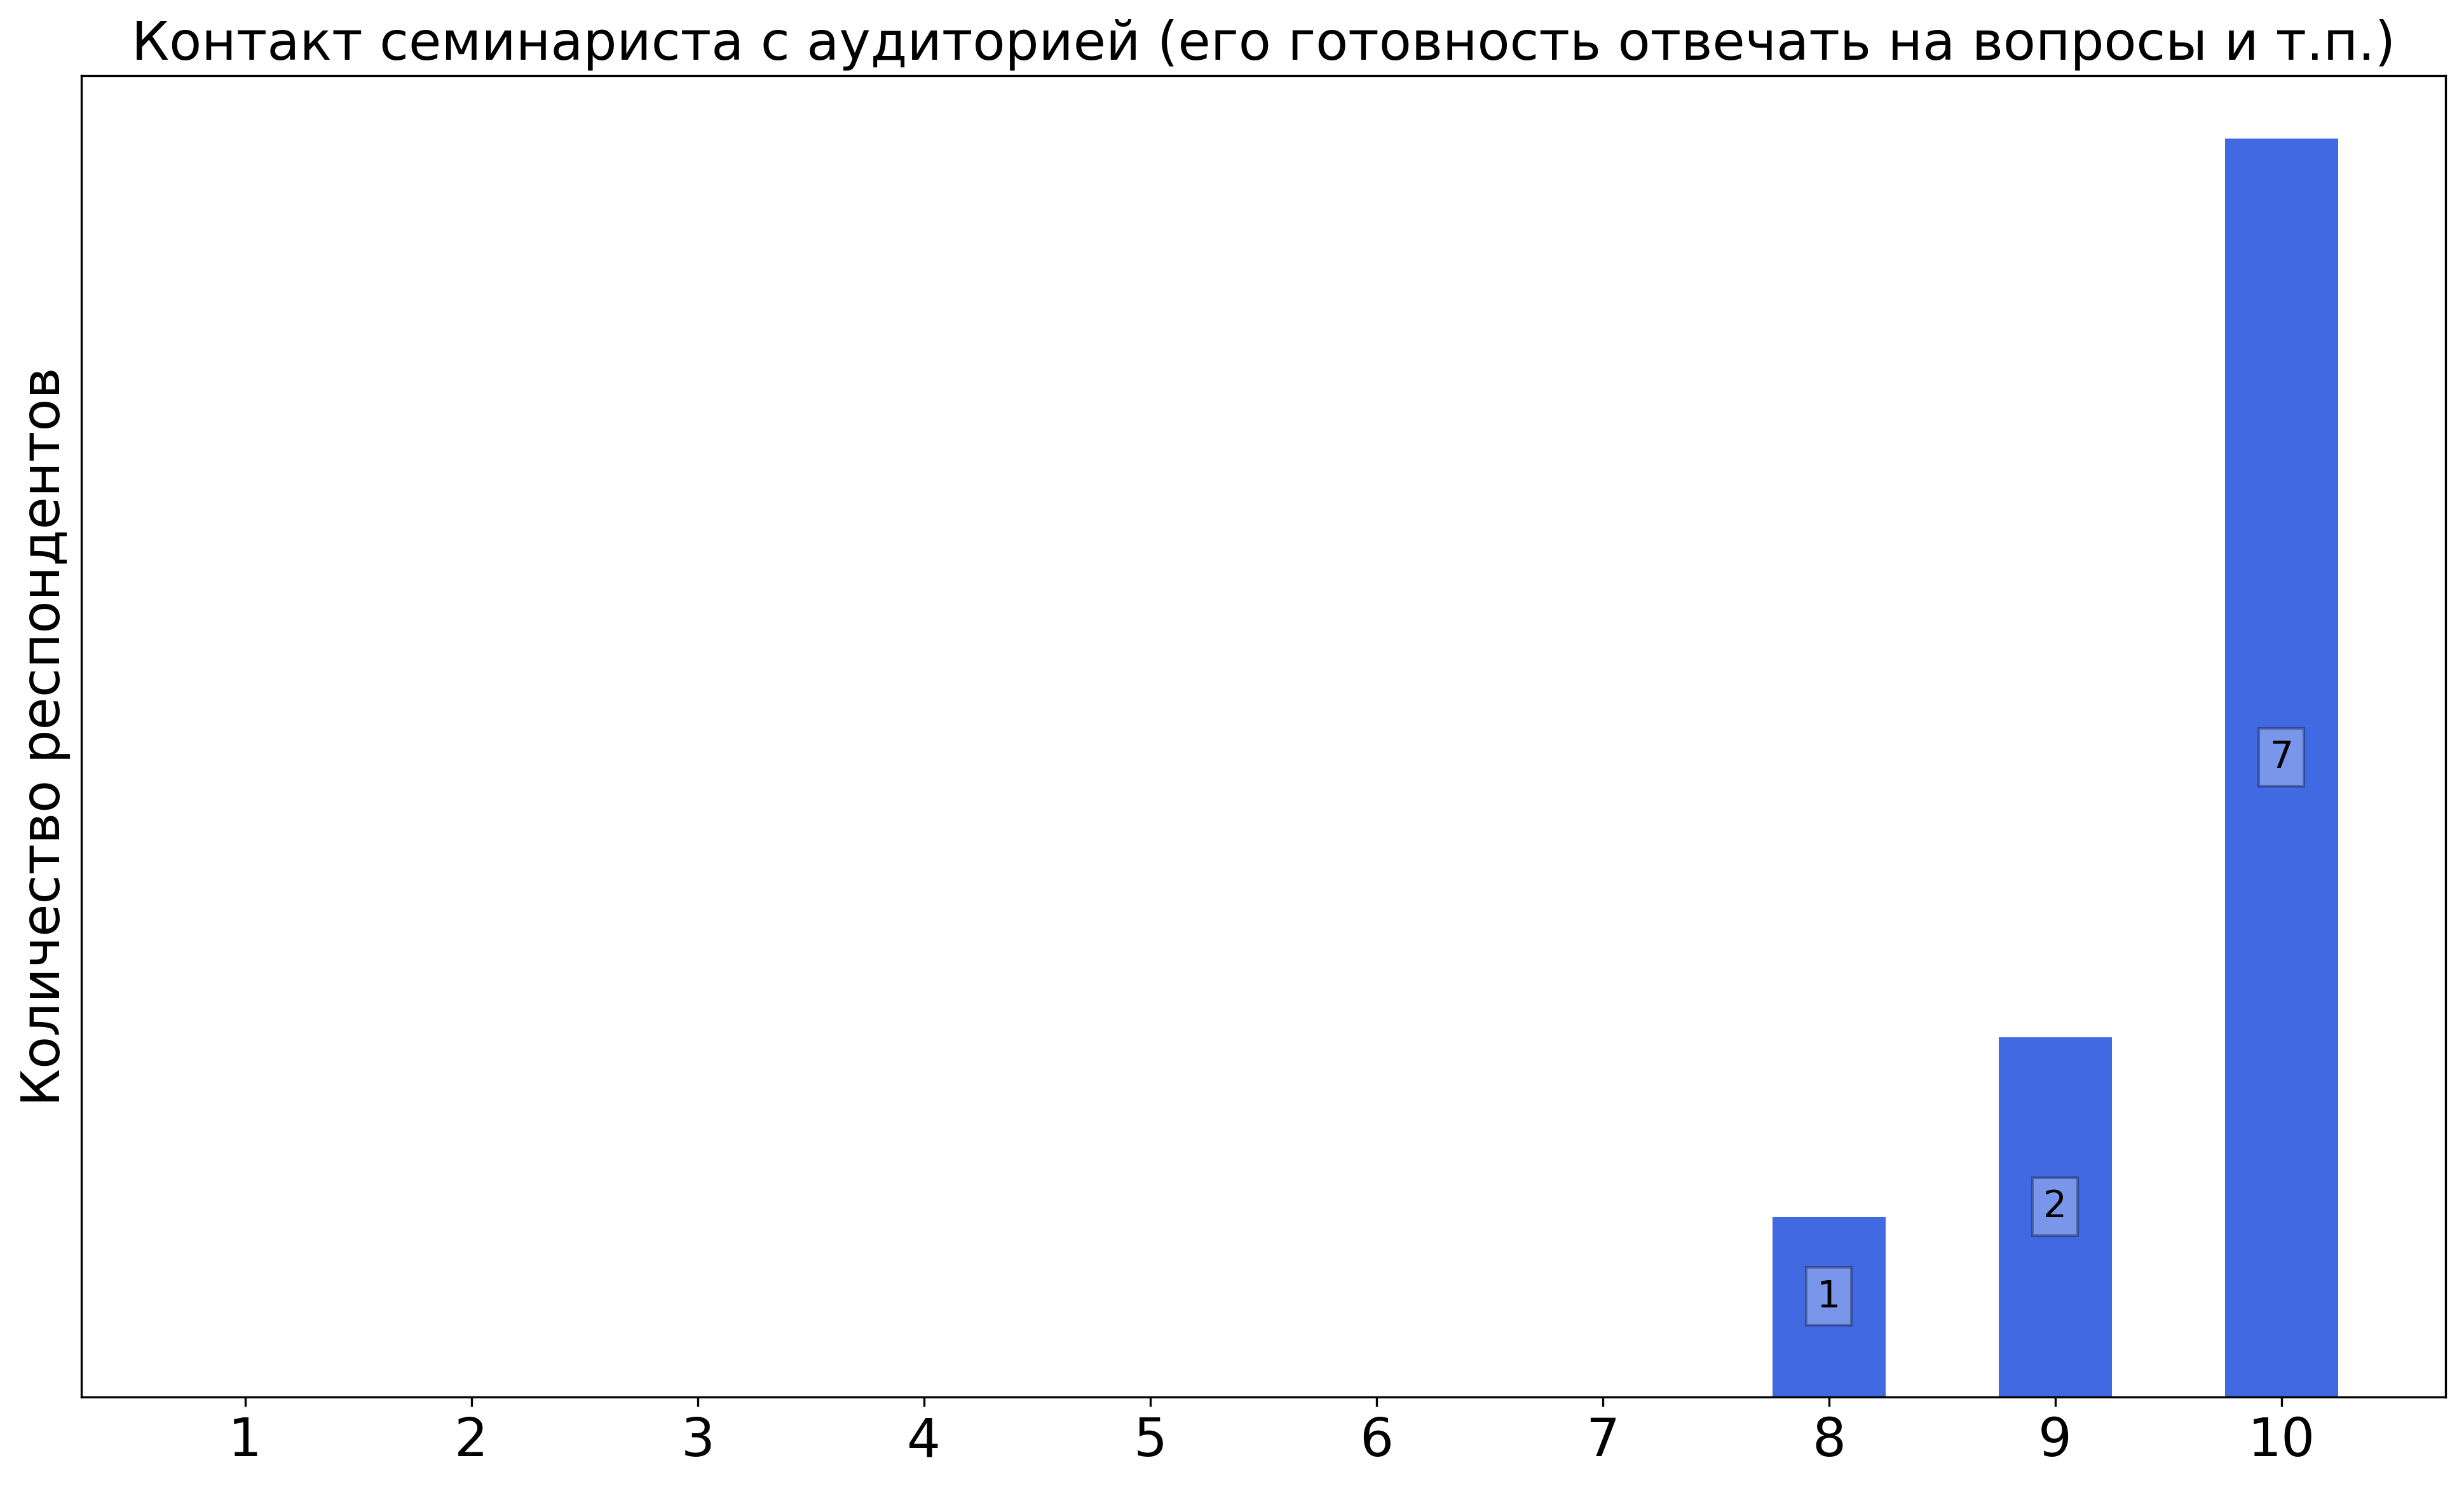
\includegraphics[width=\textwidth]{images/2 course/Кратные интегралы и теория поля/seminarists-marks-Барабанщиков А.В.-0.png}
			\end{subfigure}
			\begin{subfigure}[b]{0.45\textwidth}
				\centering
				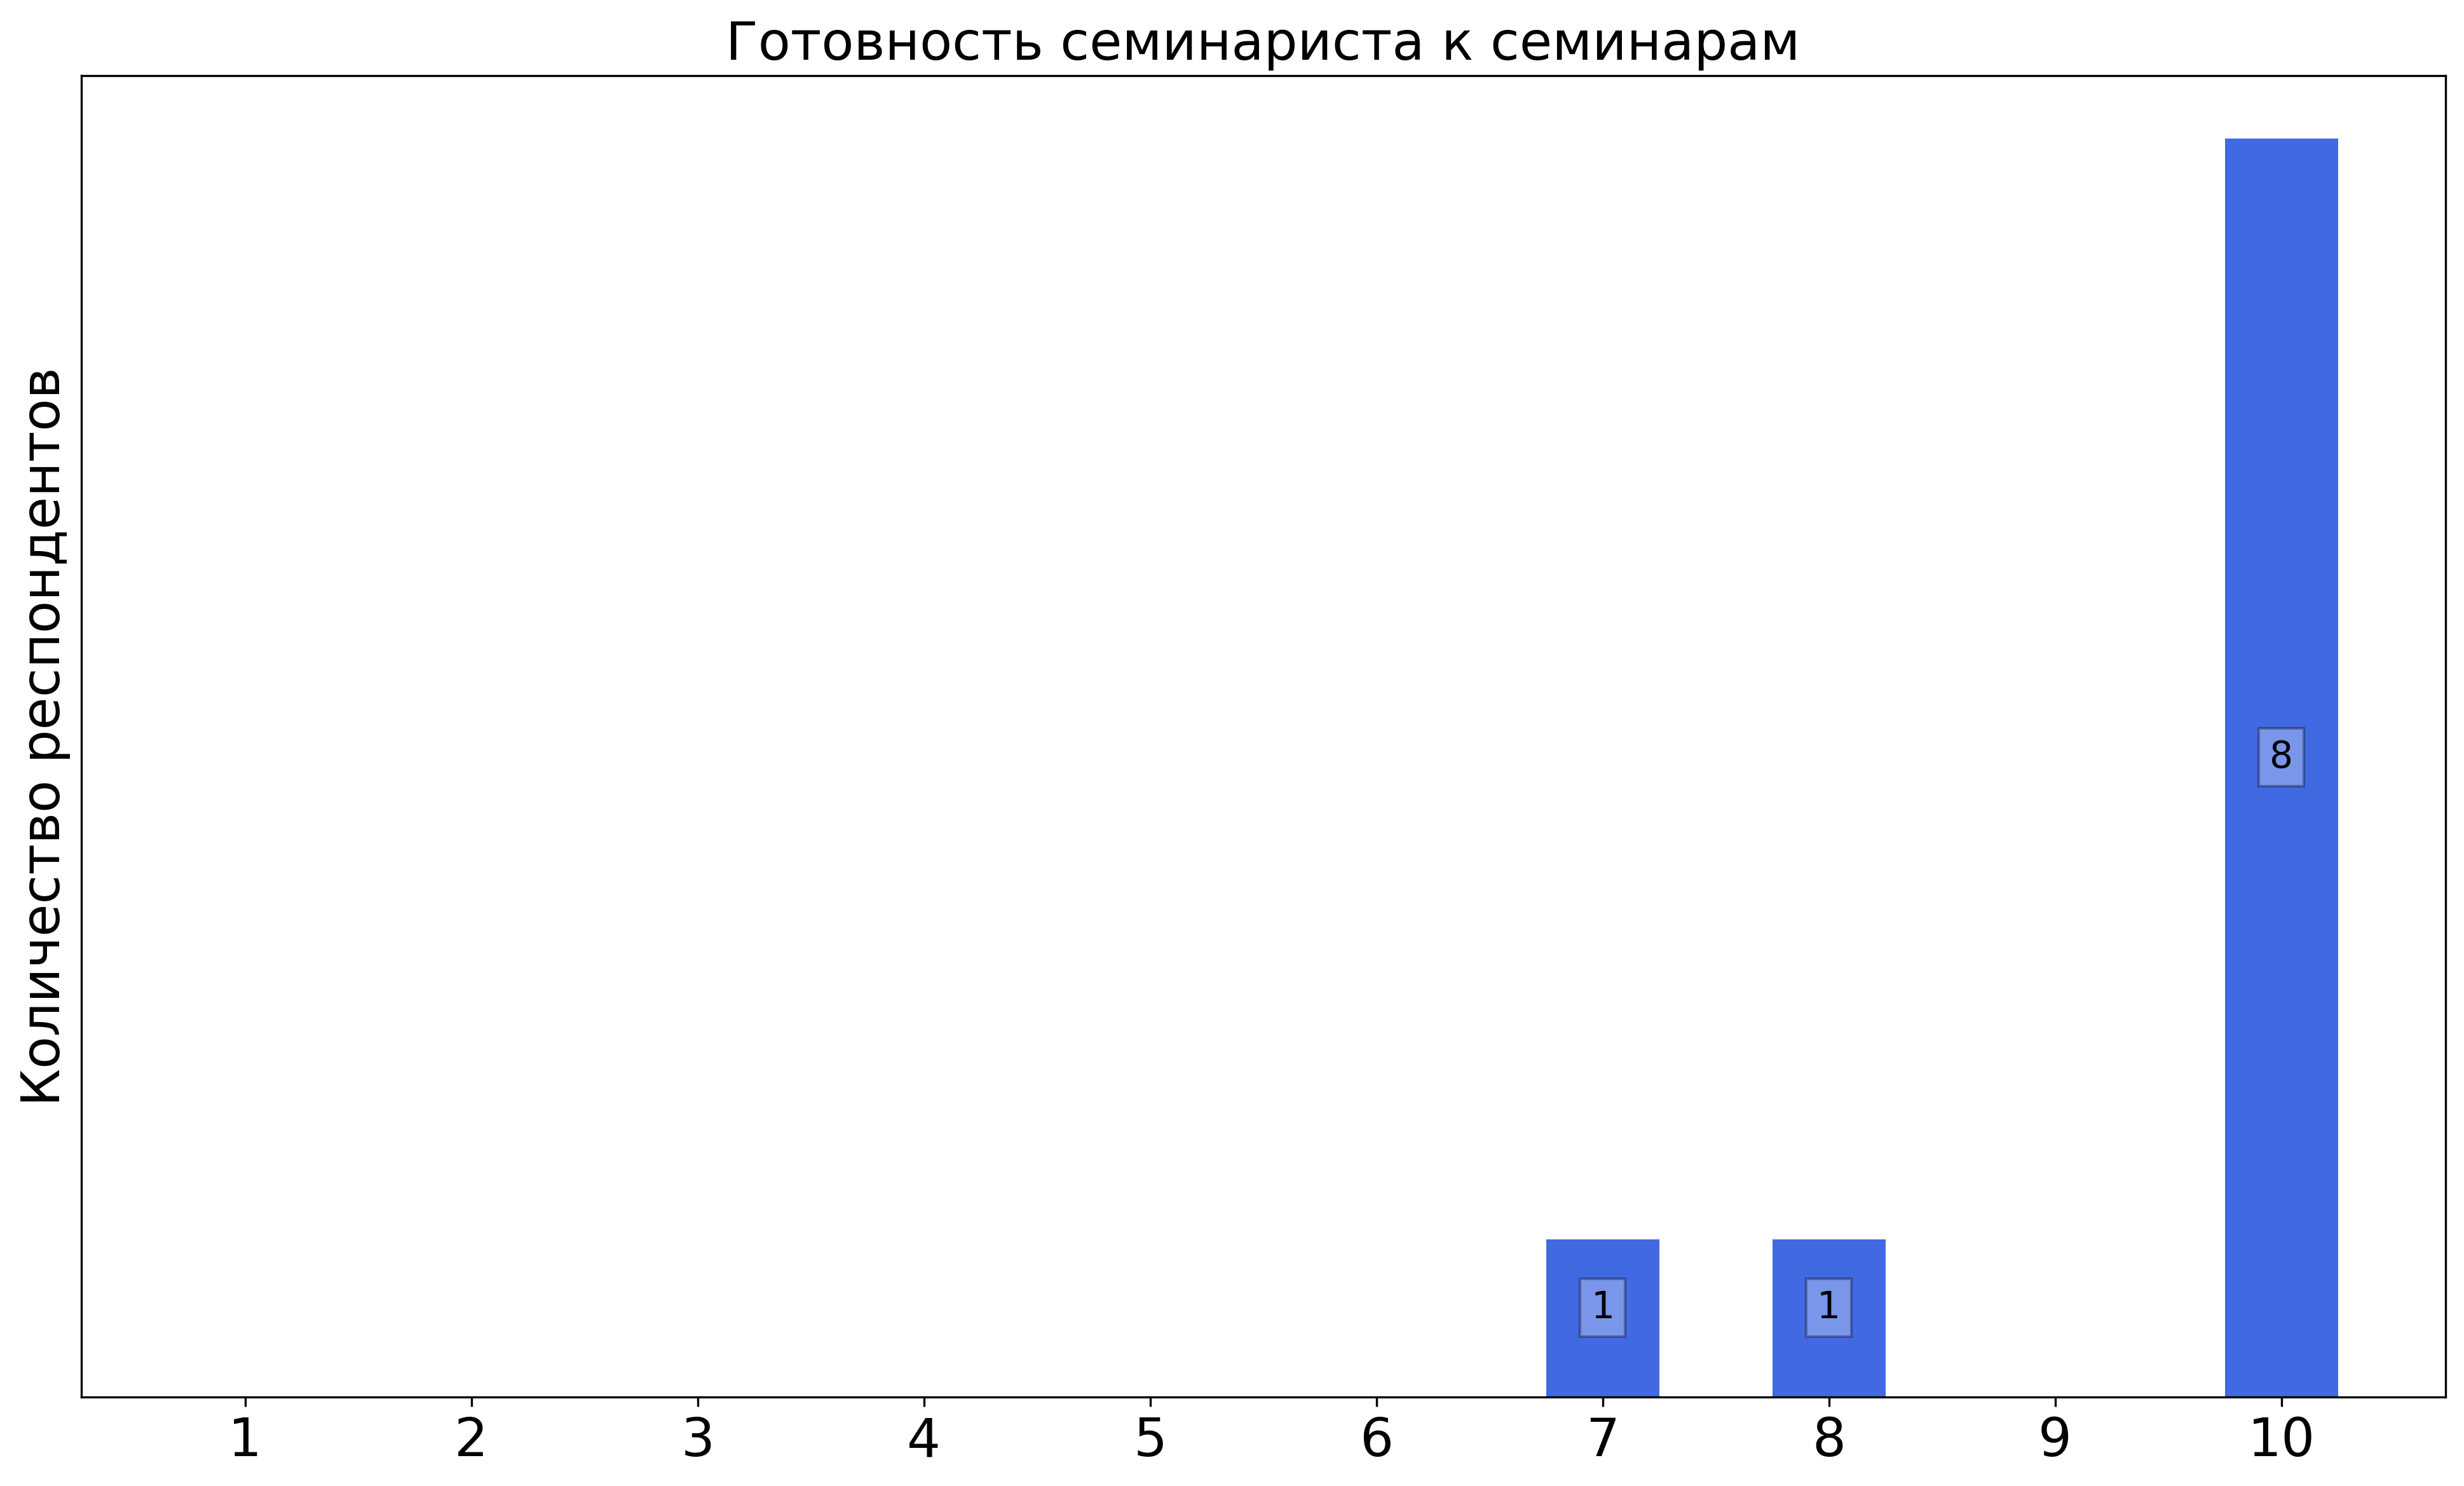
\includegraphics[width=\textwidth]{images/2 course/Кратные интегралы и теория поля/seminarists-marks-Барабанщиков А.В.-1.png}
			\end{subfigure}
			\begin{subfigure}[b]{0.45\textwidth}
				\centering
				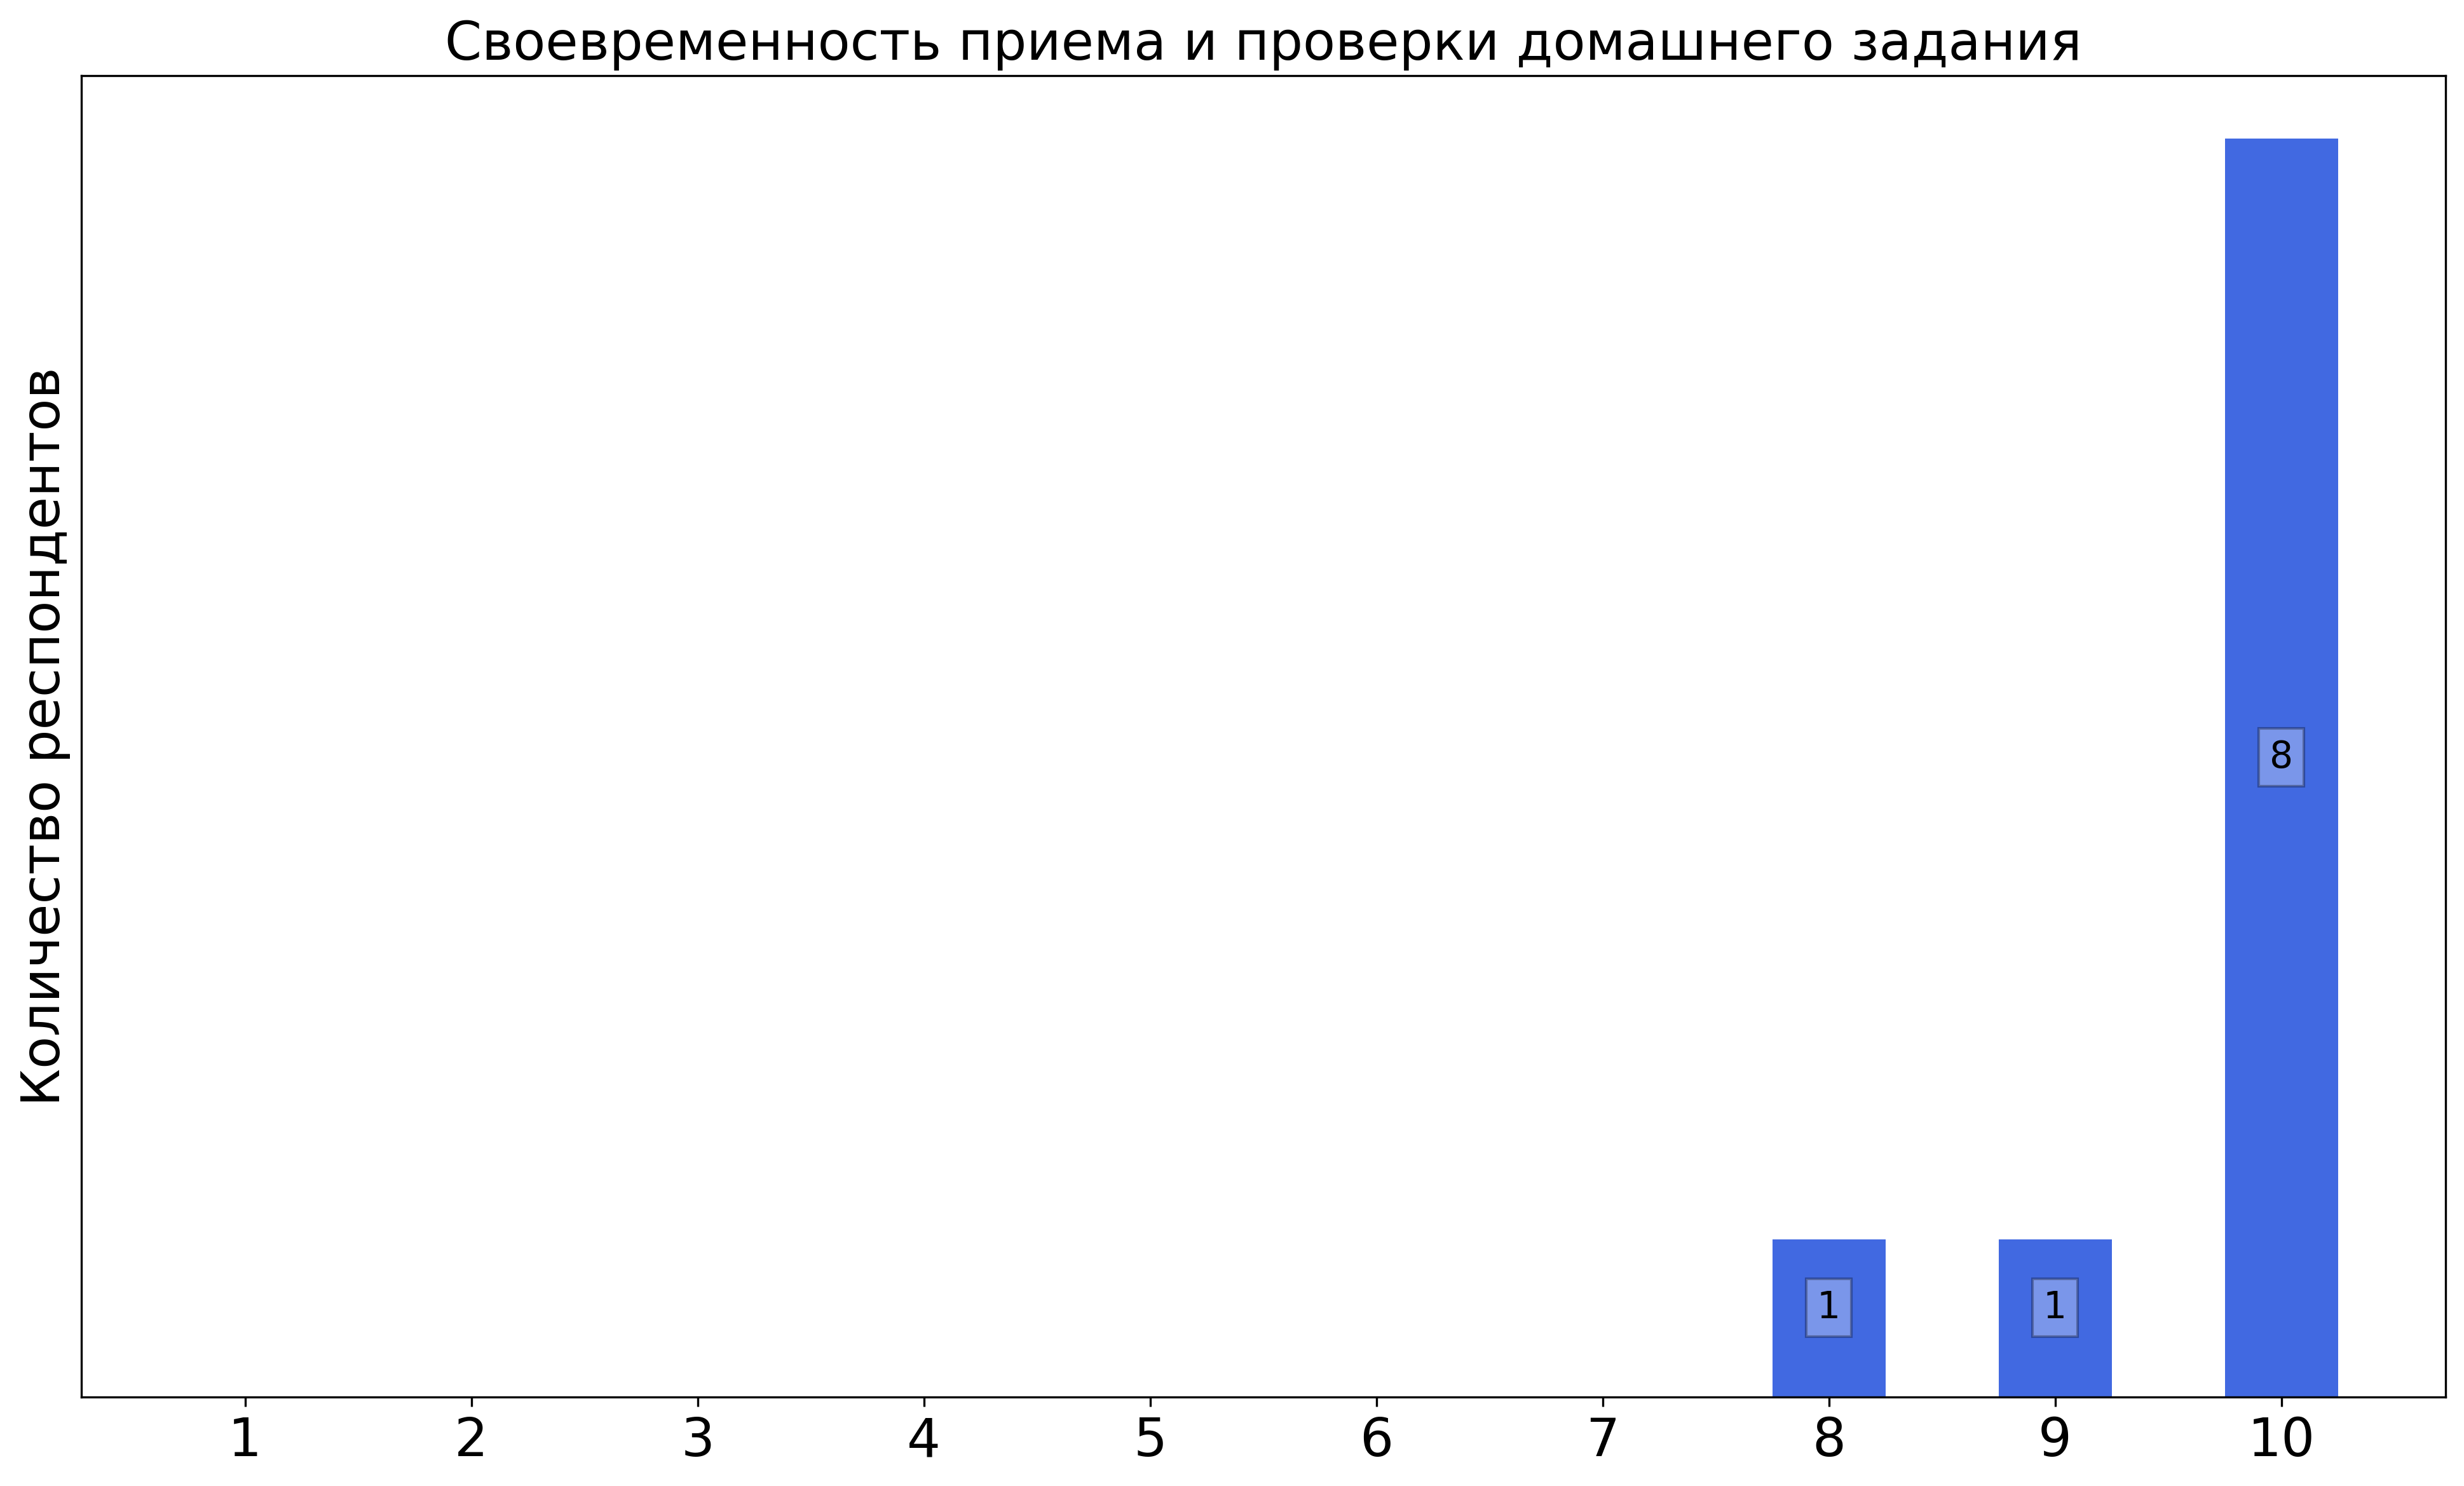
\includegraphics[width=\textwidth]{images/2 course/Кратные интегралы и теория поля/seminarists-marks-Барабанщиков А.В.-2.png}
			\end{subfigure}
			\begin{subfigure}[b]{0.45\textwidth}
				\centering
				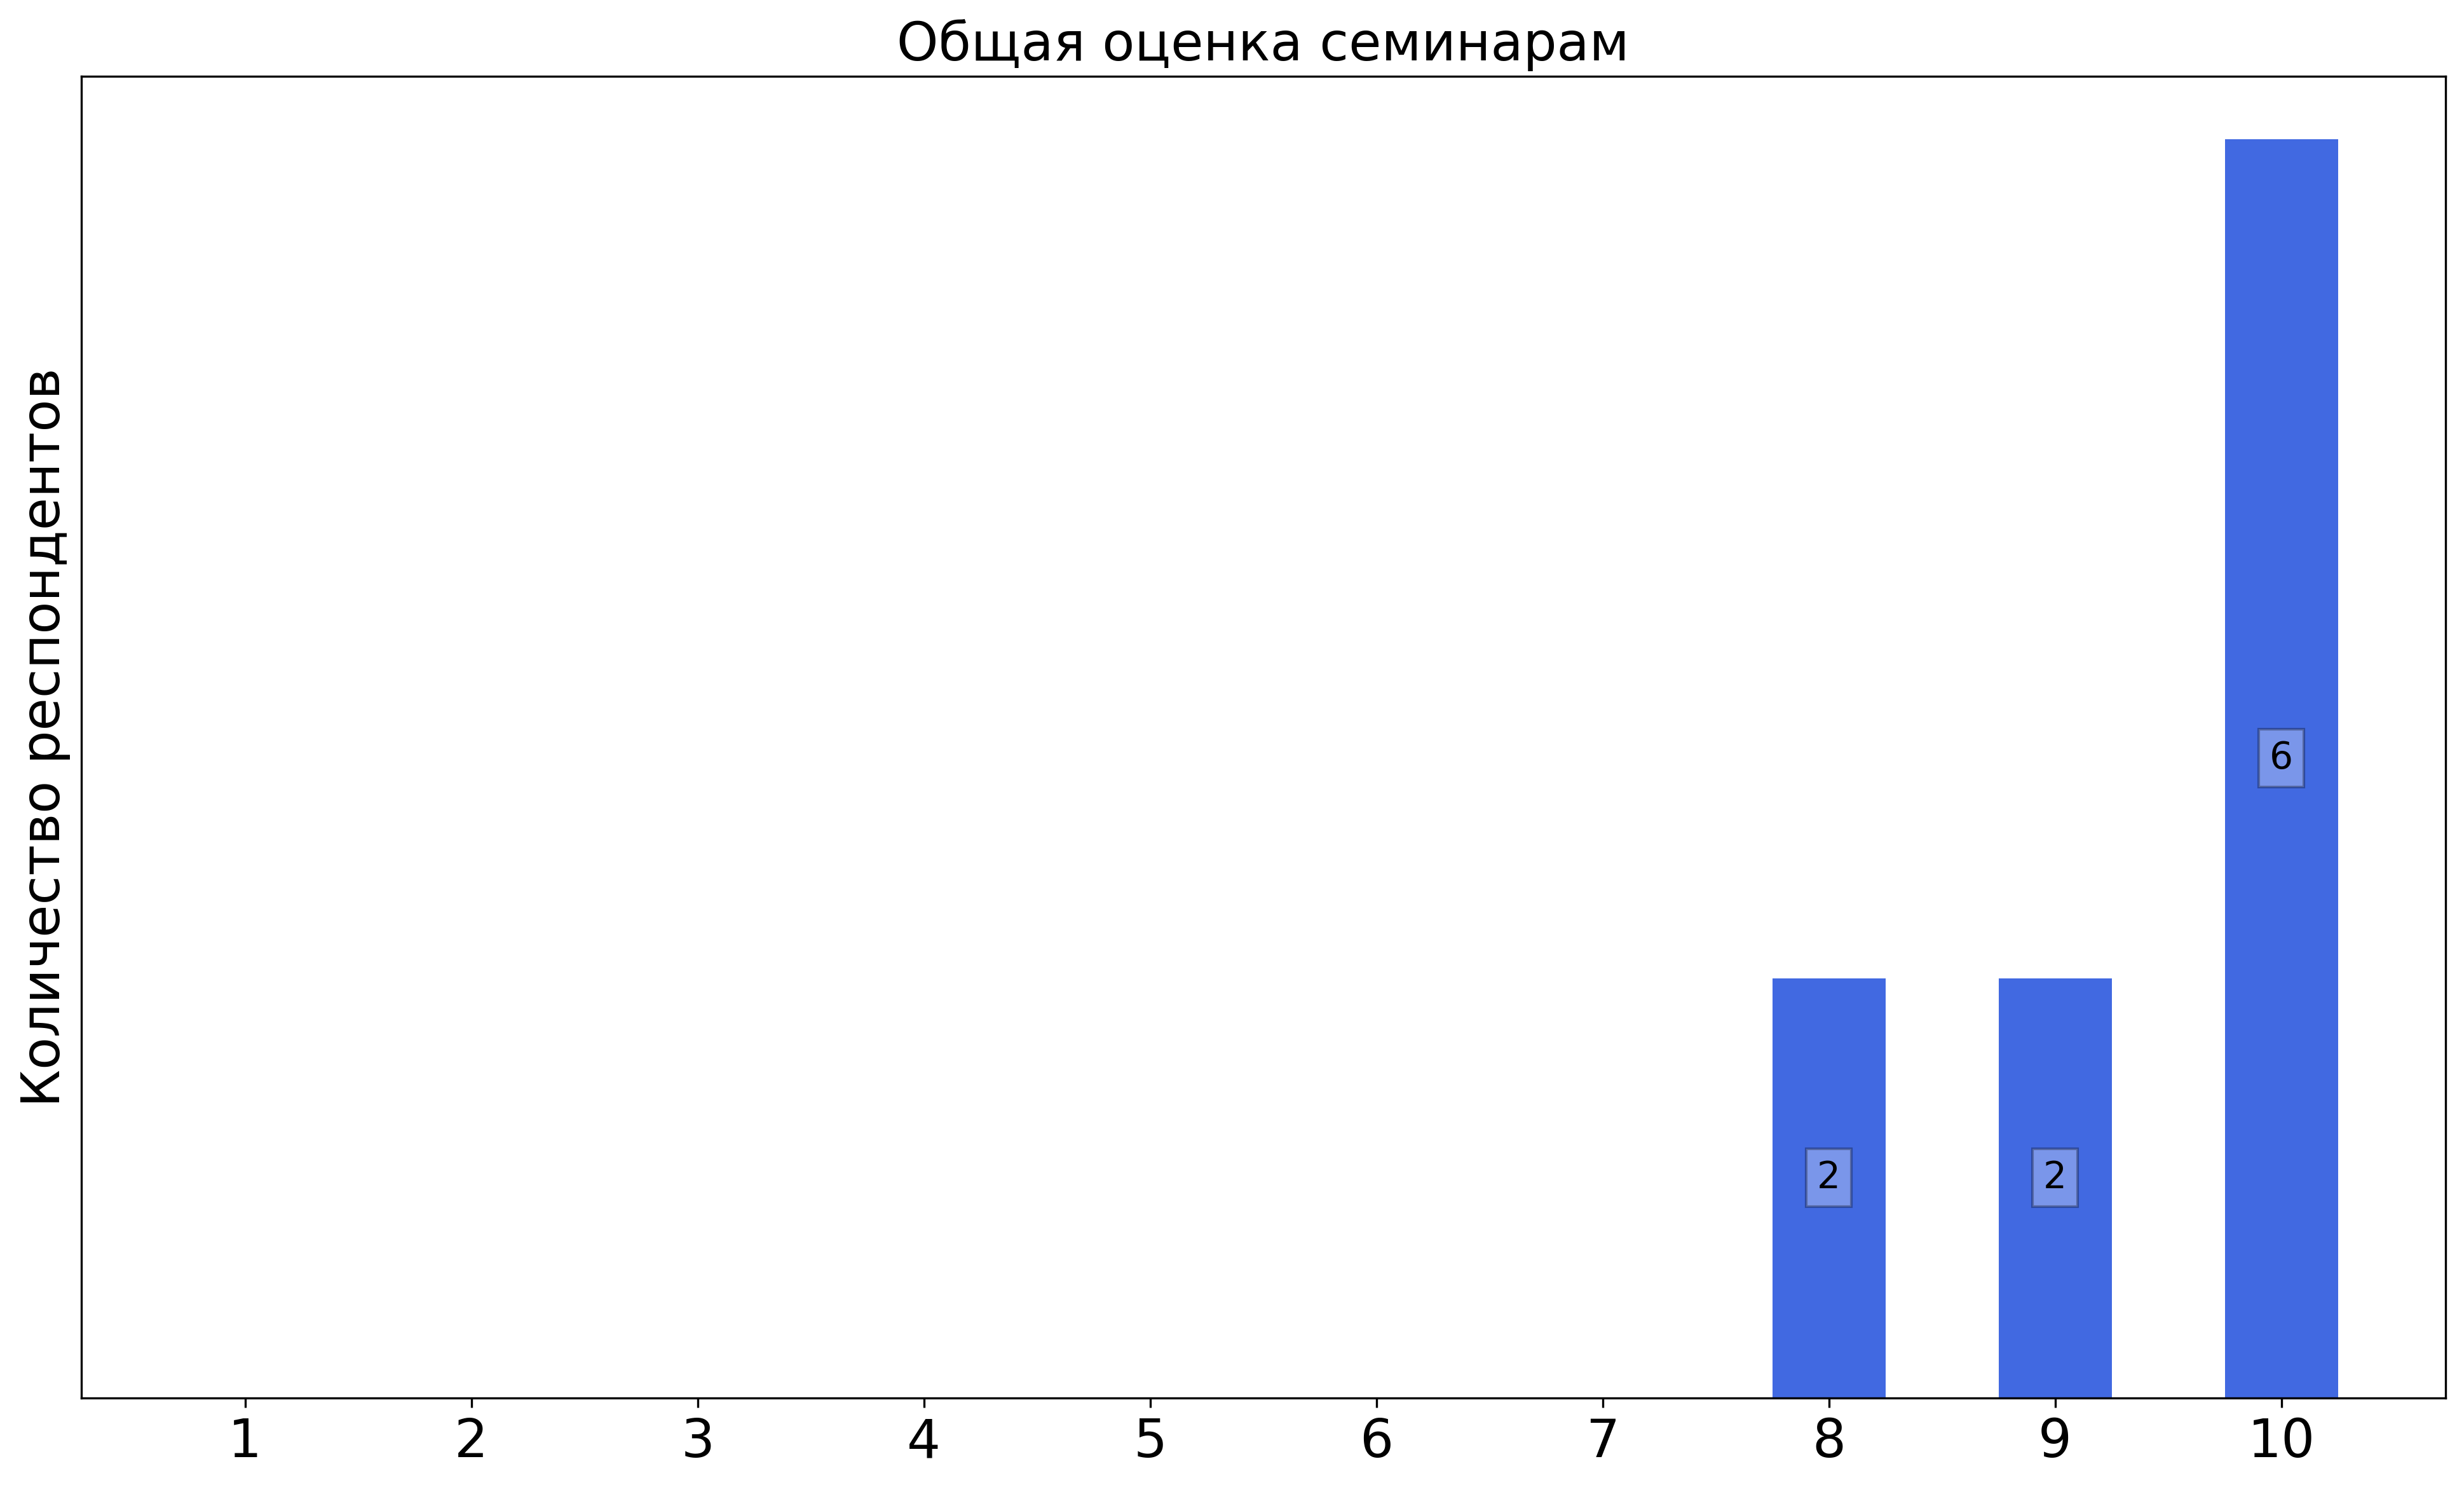
\includegraphics[width=\textwidth]{images/2 course/Кратные интегралы и теория поля/seminarists-marks-Барабанщиков А.В.-3.png}
			\end{subfigure}	
			\caption{Оценки респондентов о качестве преподавания семинаров}
		\end{figure}

		\textbf{Комментарии студентов о семинаристе\protect\footnote{сохранены оригинальные орфография и пунктуация}}
            \begin{commentbox} 
                Было крайне полезно посещать данные семинары 
            \end{commentbox} 
        
            \begin{commentbox} 
                Замечательный преподаватель и человек 
            \end{commentbox} 
        
        
    \subsubsection{Отзыв студентов о семинарах. Семинарист: Бишаев А.М.}
		\begin{figure}[H]
			\centering
			\begin{subfigure}[b]{0.45\textwidth}
				\centering
				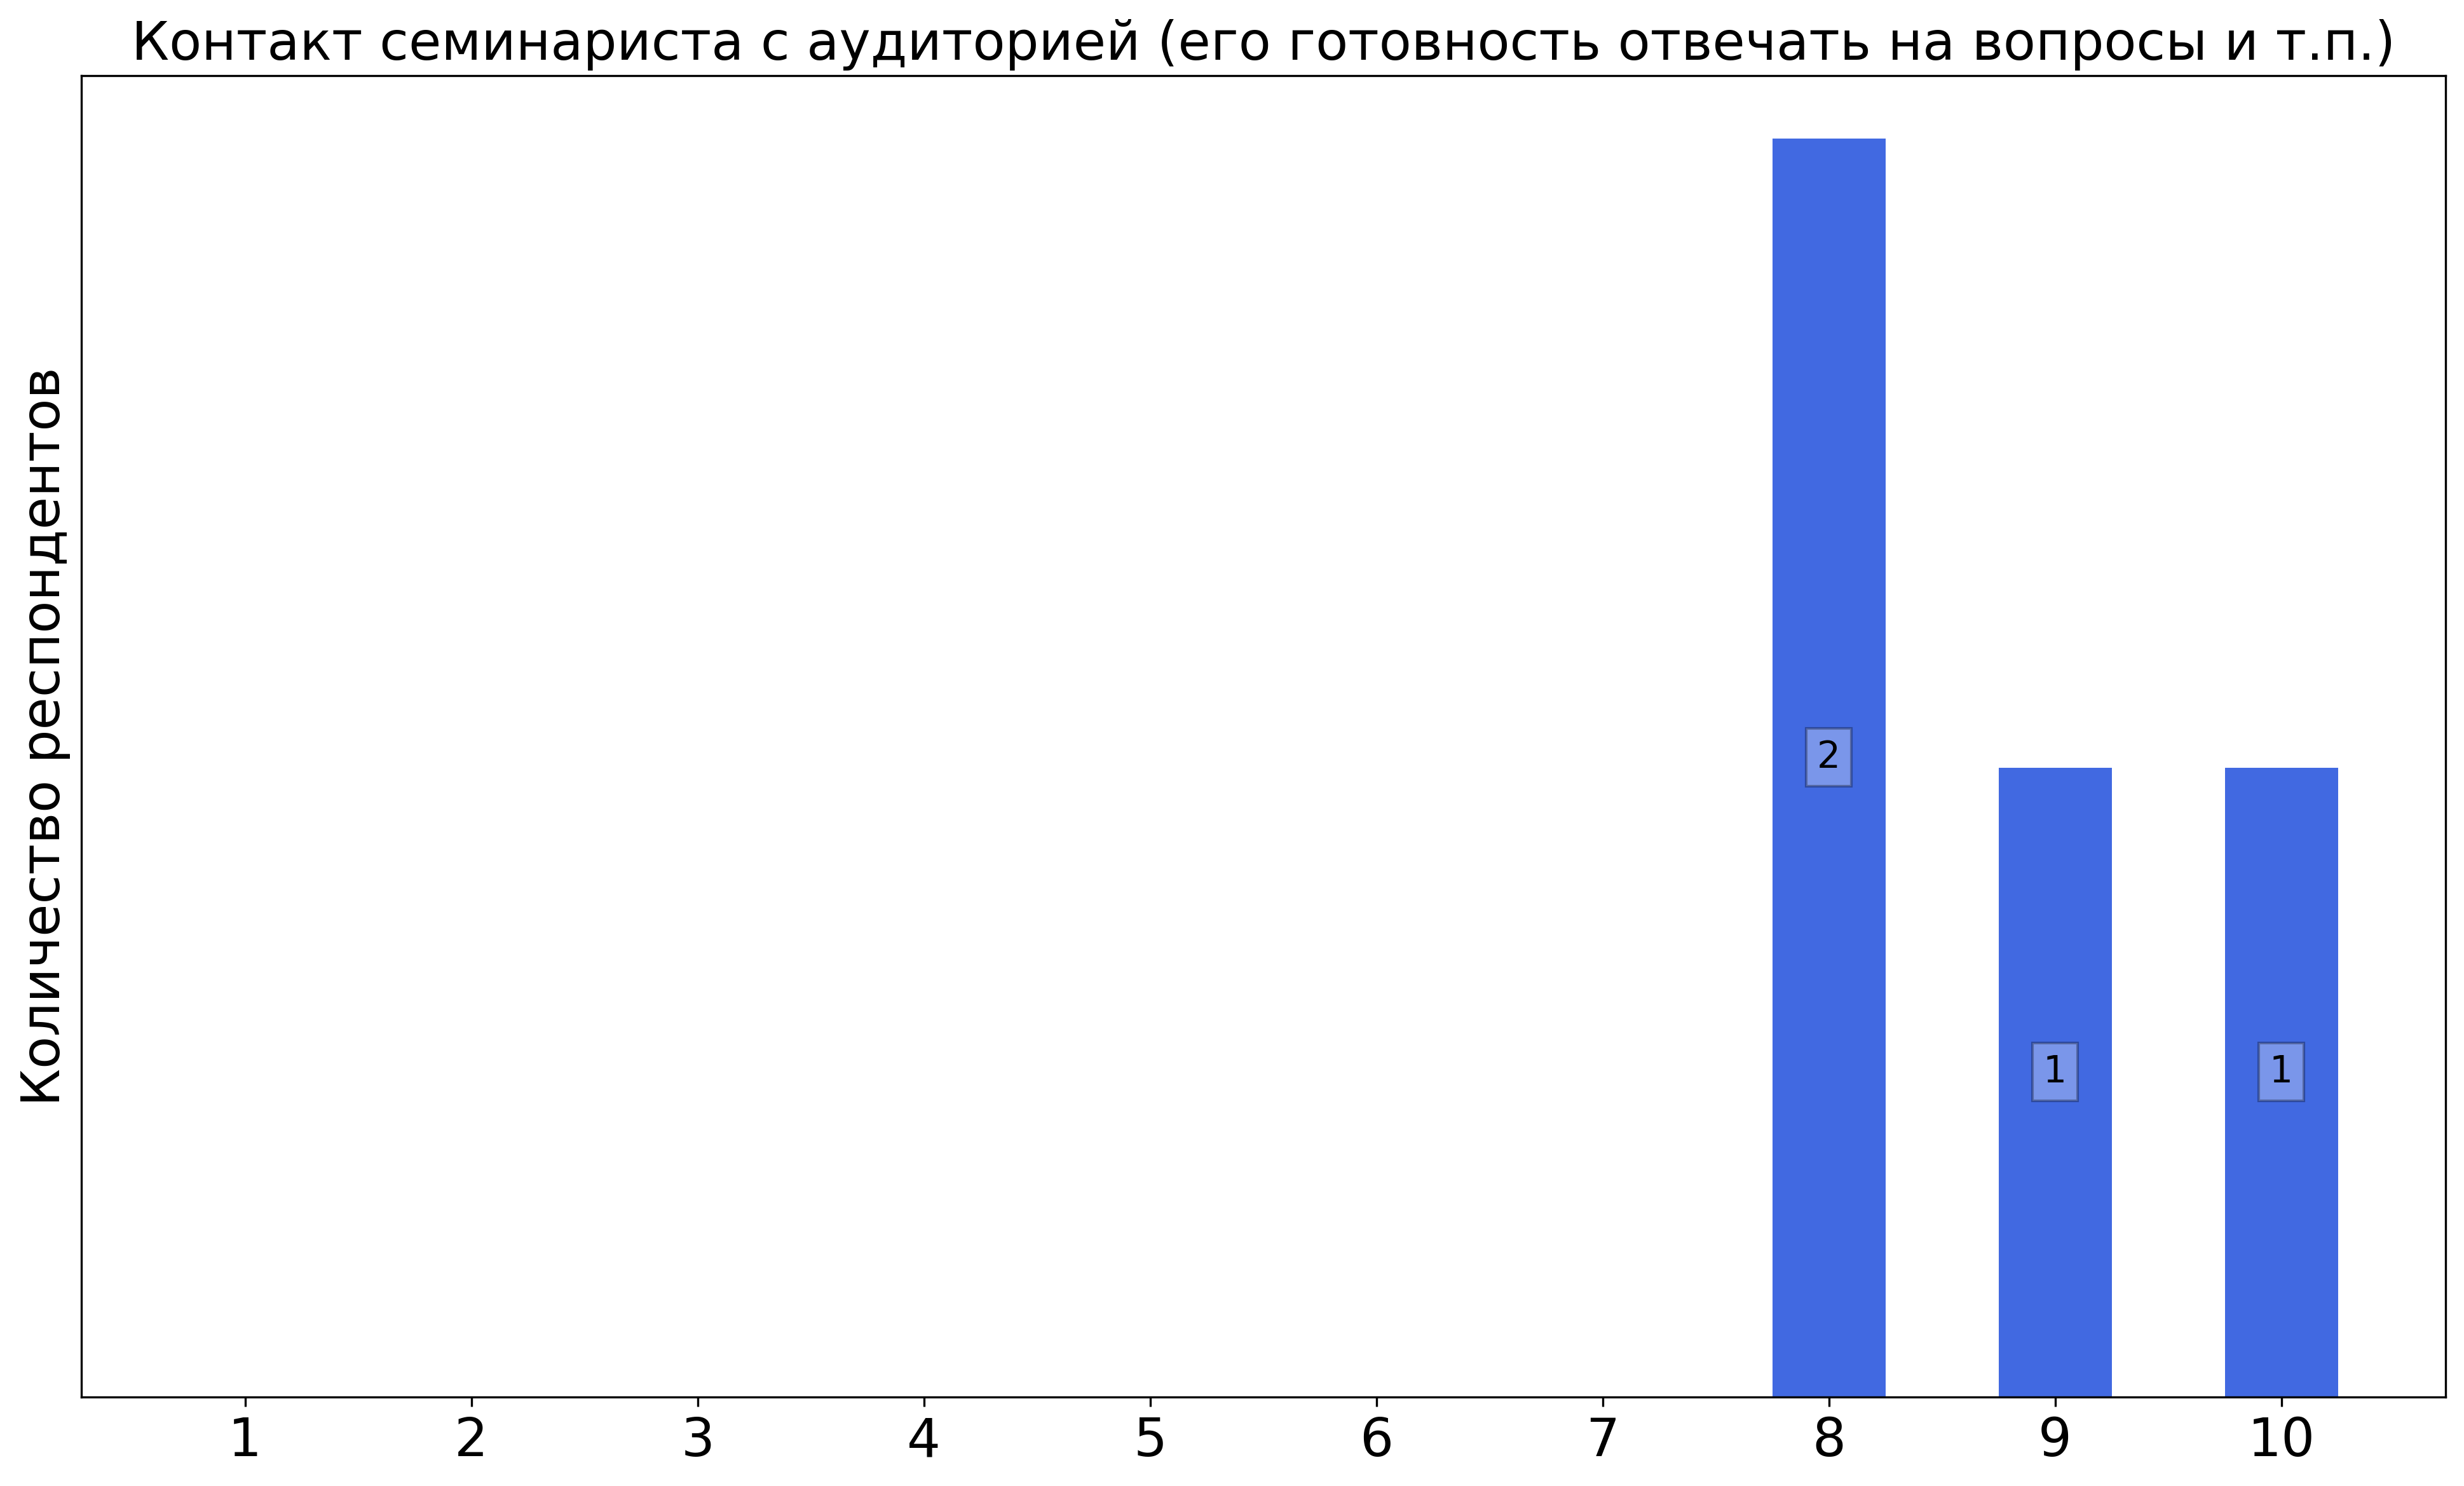
\includegraphics[width=\textwidth]{images/2 course/Кратные интегралы и теория поля/seminarists-marks-Бишаев А.М.-0.png}
			\end{subfigure}
			\begin{subfigure}[b]{0.45\textwidth}
				\centering
				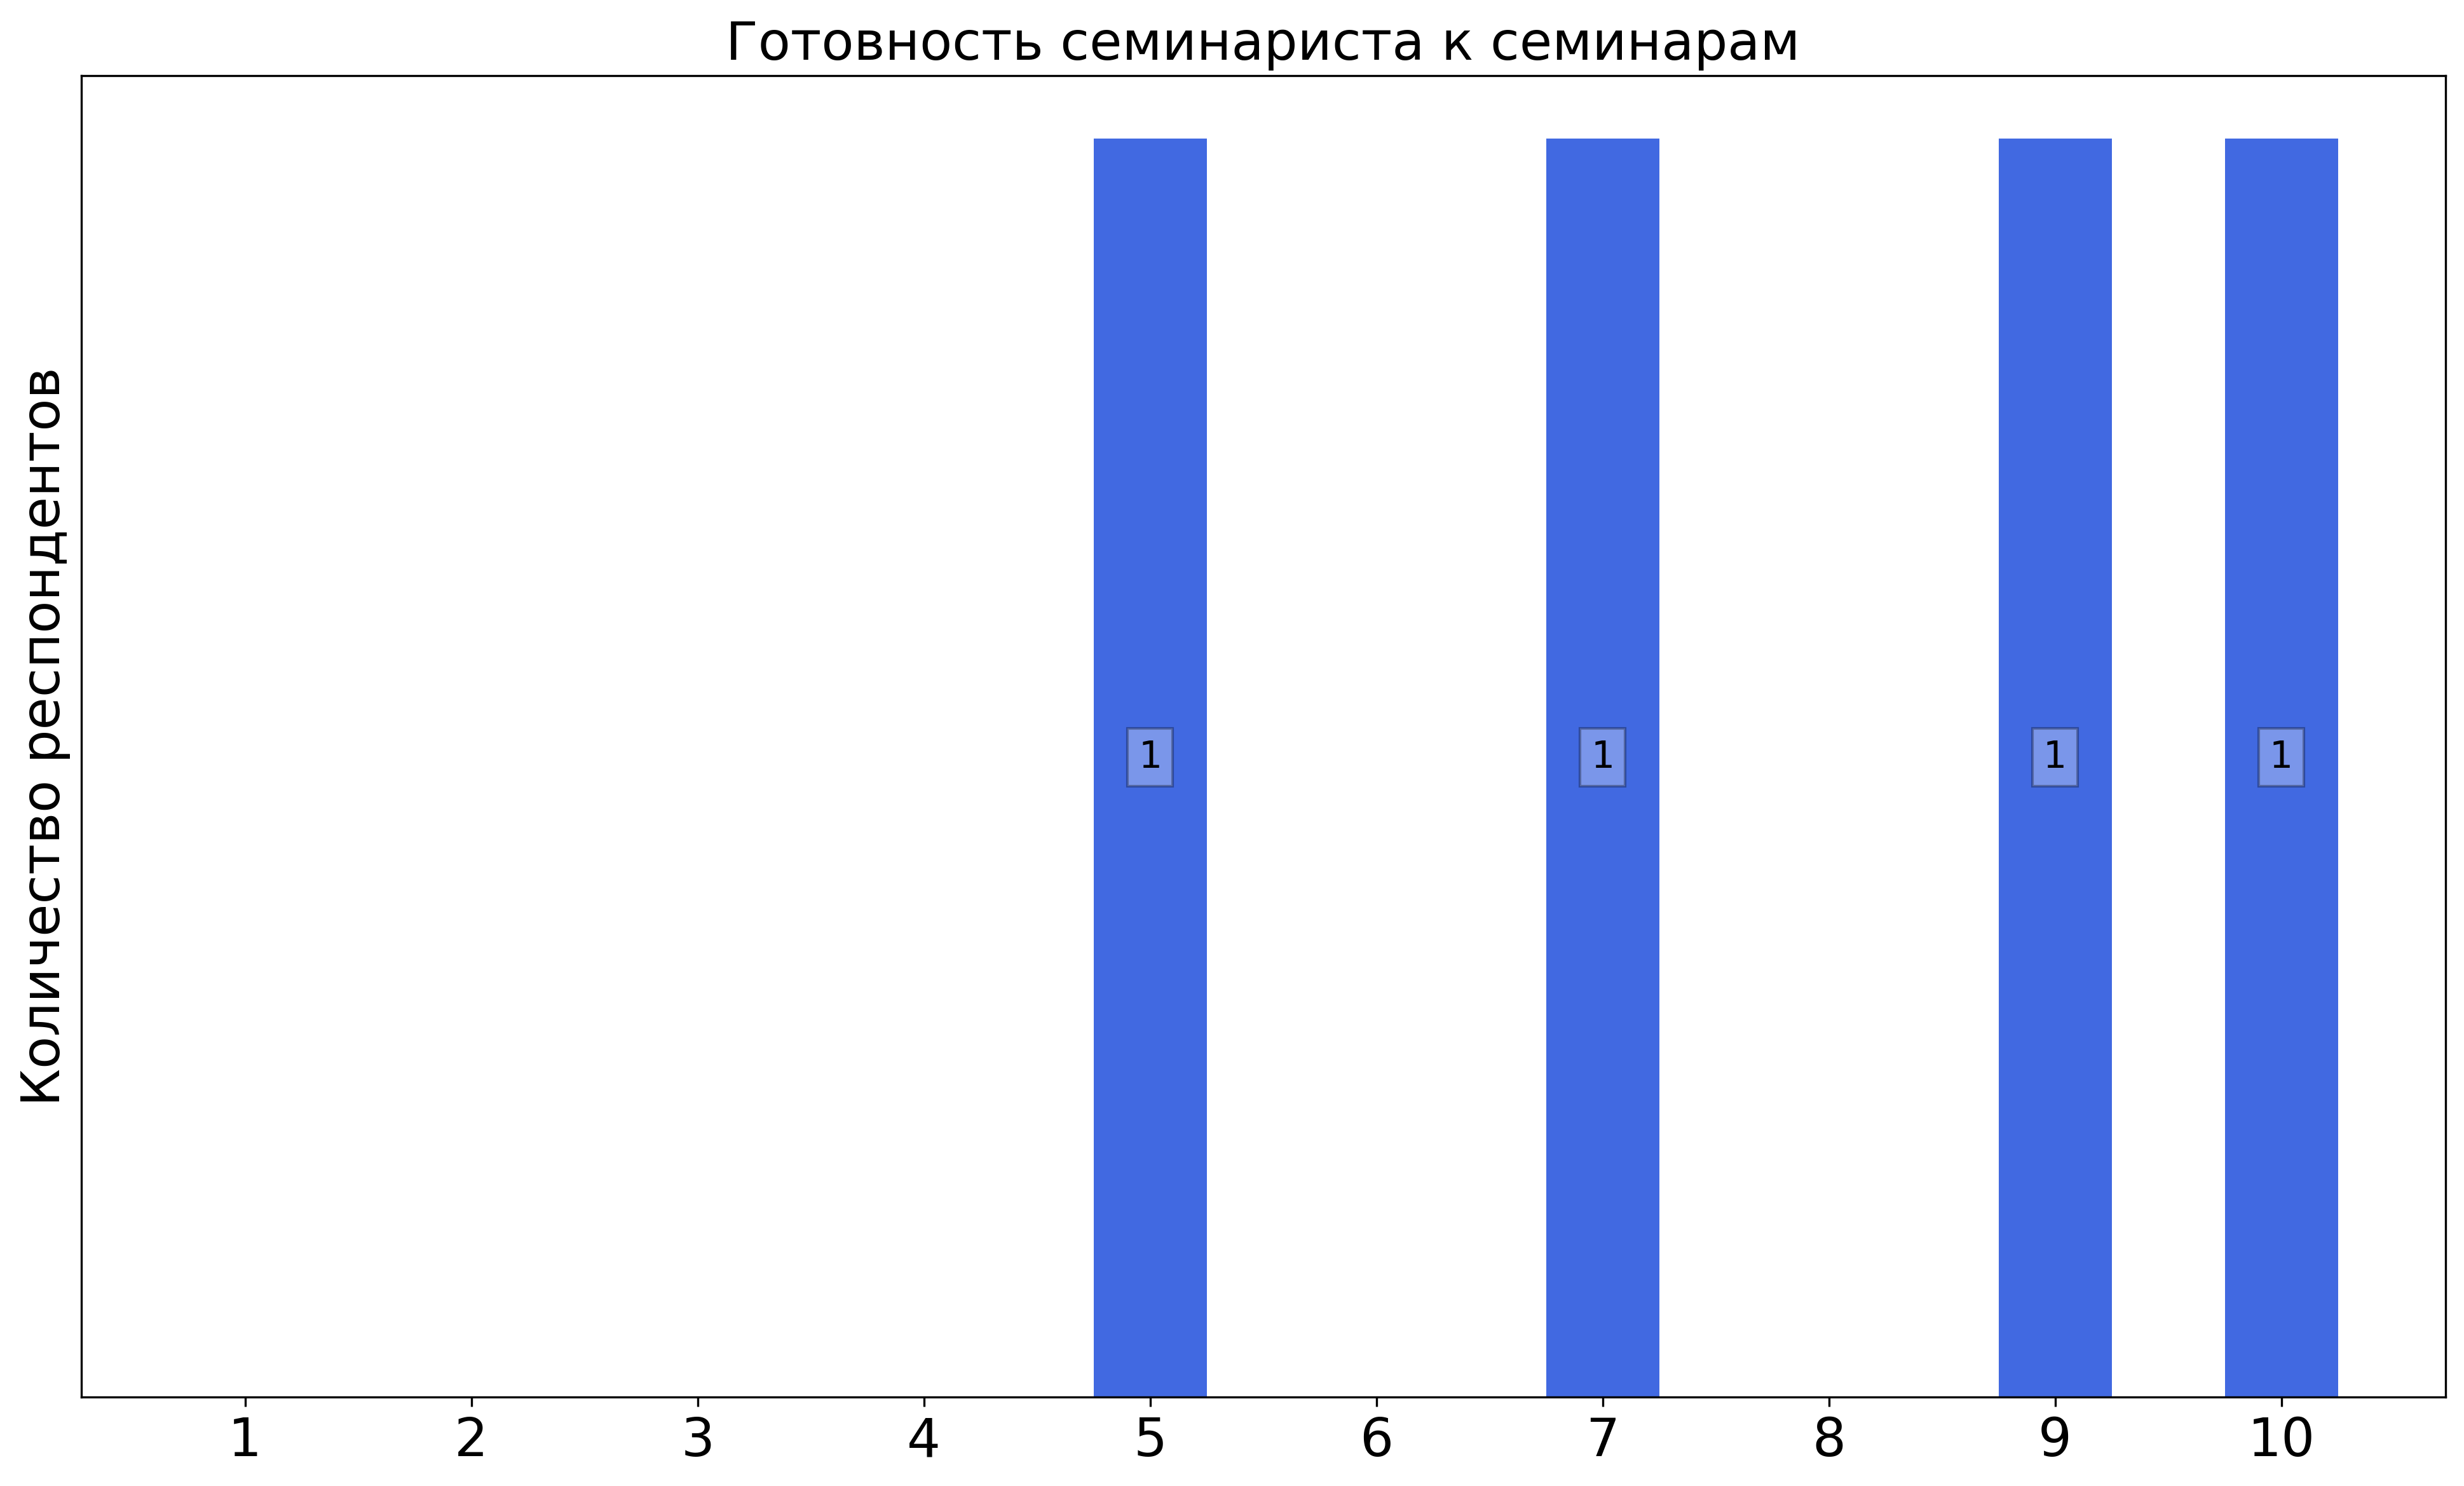
\includegraphics[width=\textwidth]{images/2 course/Кратные интегралы и теория поля/seminarists-marks-Бишаев А.М.-1.png}
			\end{subfigure}
			\begin{subfigure}[b]{0.45\textwidth}
				\centering
				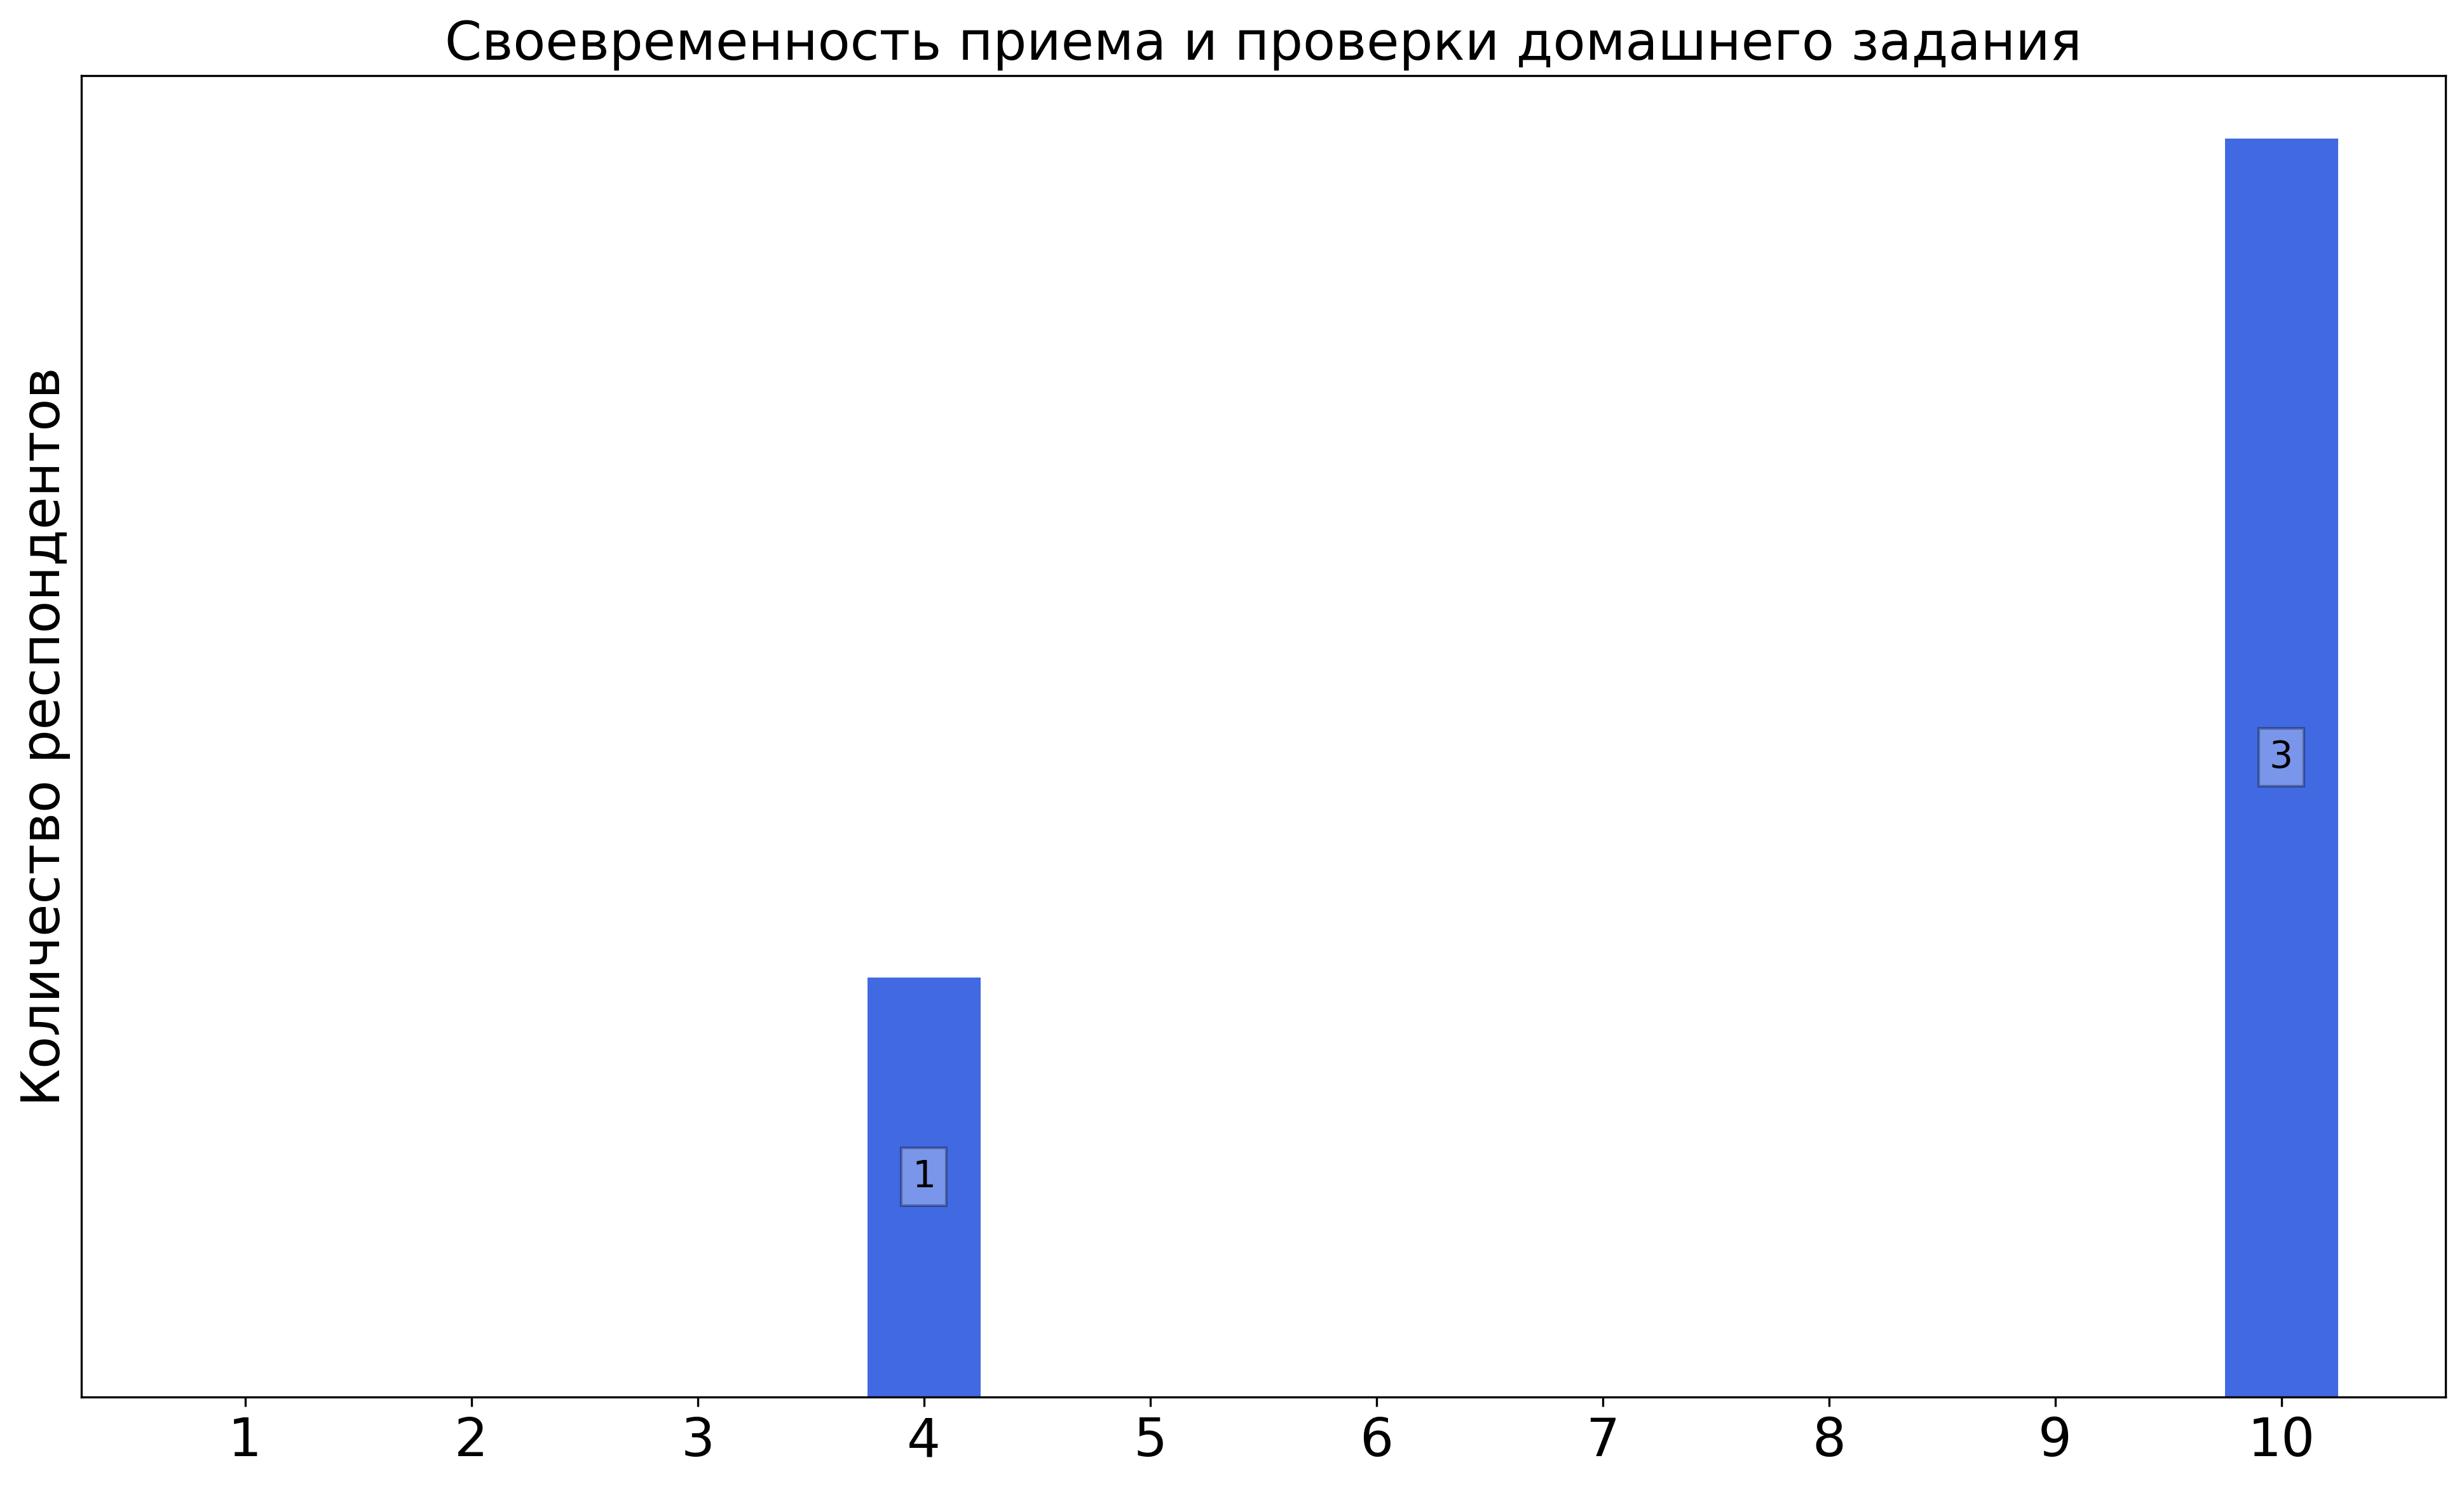
\includegraphics[width=\textwidth]{images/2 course/Кратные интегралы и теория поля/seminarists-marks-Бишаев А.М.-2.png}
			\end{subfigure}
			\begin{subfigure}[b]{0.45\textwidth}
				\centering
				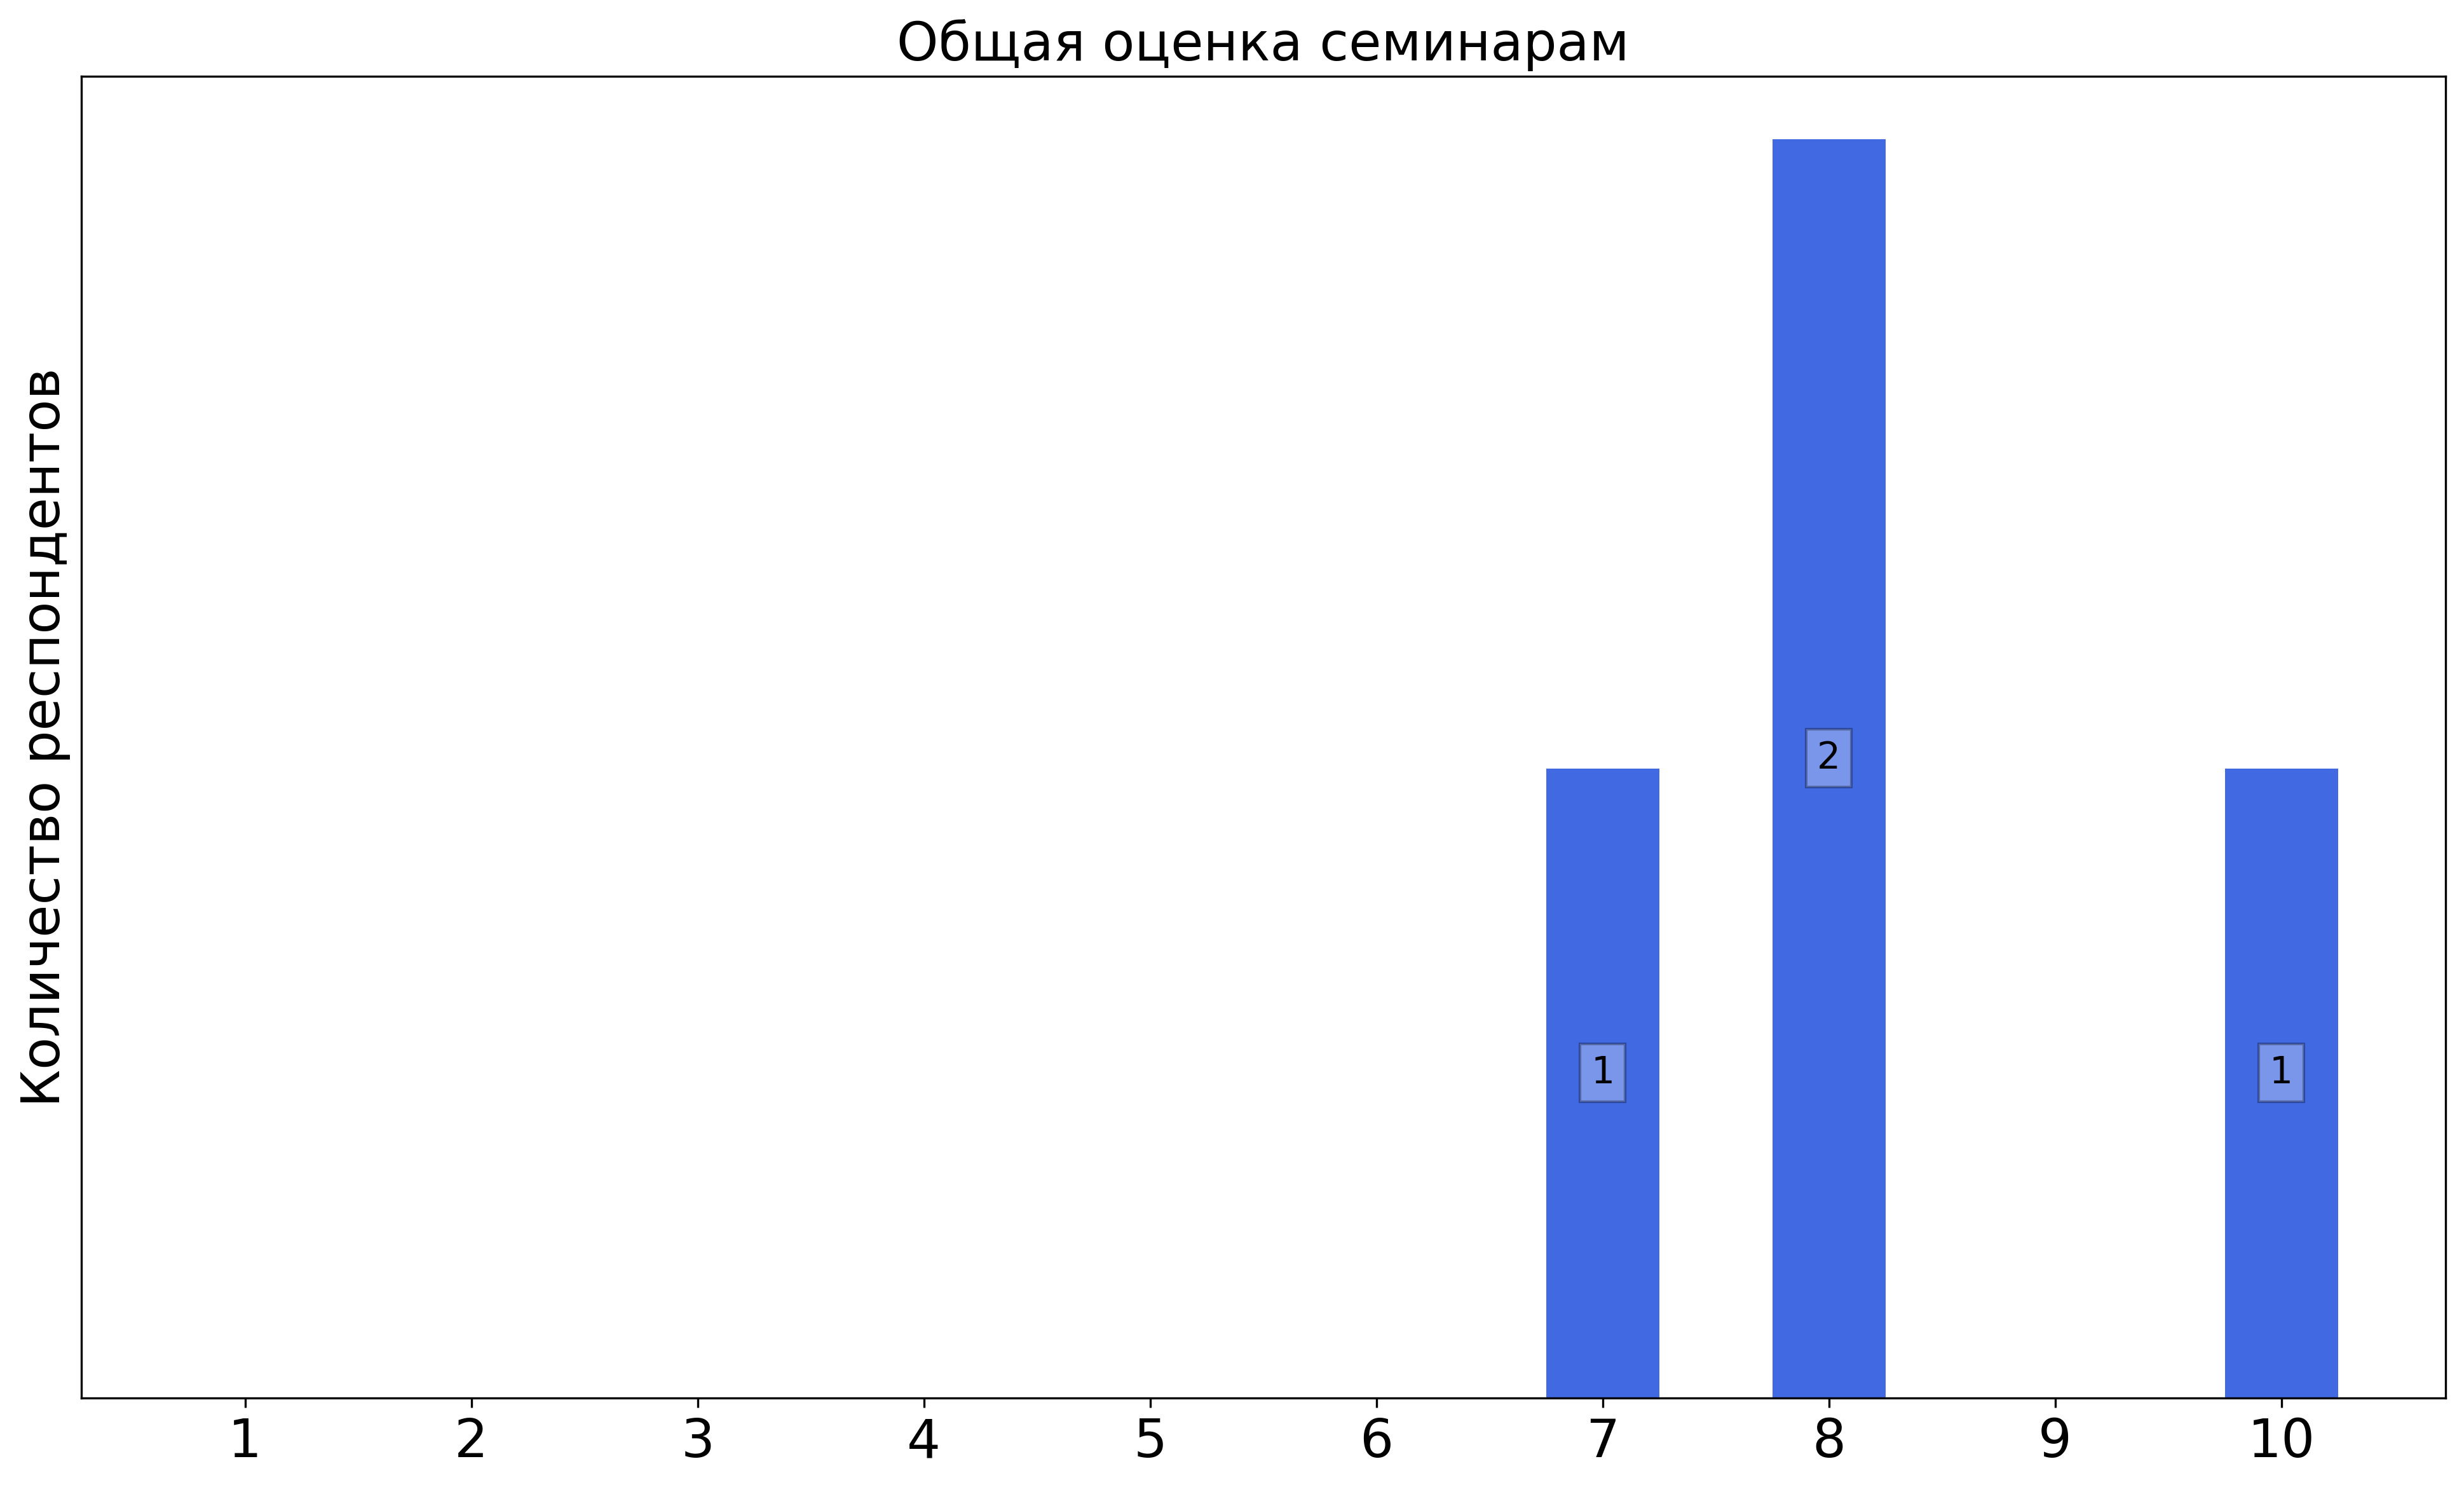
\includegraphics[width=\textwidth]{images/2 course/Кратные интегралы и теория поля/seminarists-marks-Бишаев А.М.-3.png}
			\end{subfigure}	
			\caption{Оценки респондентов о качестве преподавания семинаров}
		\end{figure}

		\textbf{Комментарии студентов о семинаристе\protect\footnote{сохранены оригинальные орфография и пунктуация}}
            \begin{commentbox} 
                Александр Михайлович достаточно специфично ведёт материал. Его часто приходится поправлять на ошибки, что не уменьшает количество проходимого материала  
            \end{commentbox} 
        
            
    \subsubsection{Отзыв студентов о семинарах. Семинарист: Петрович А.Ю.}
		\begin{figure}[H]
			\centering
			\begin{subfigure}[b]{0.45\textwidth}
				\centering
				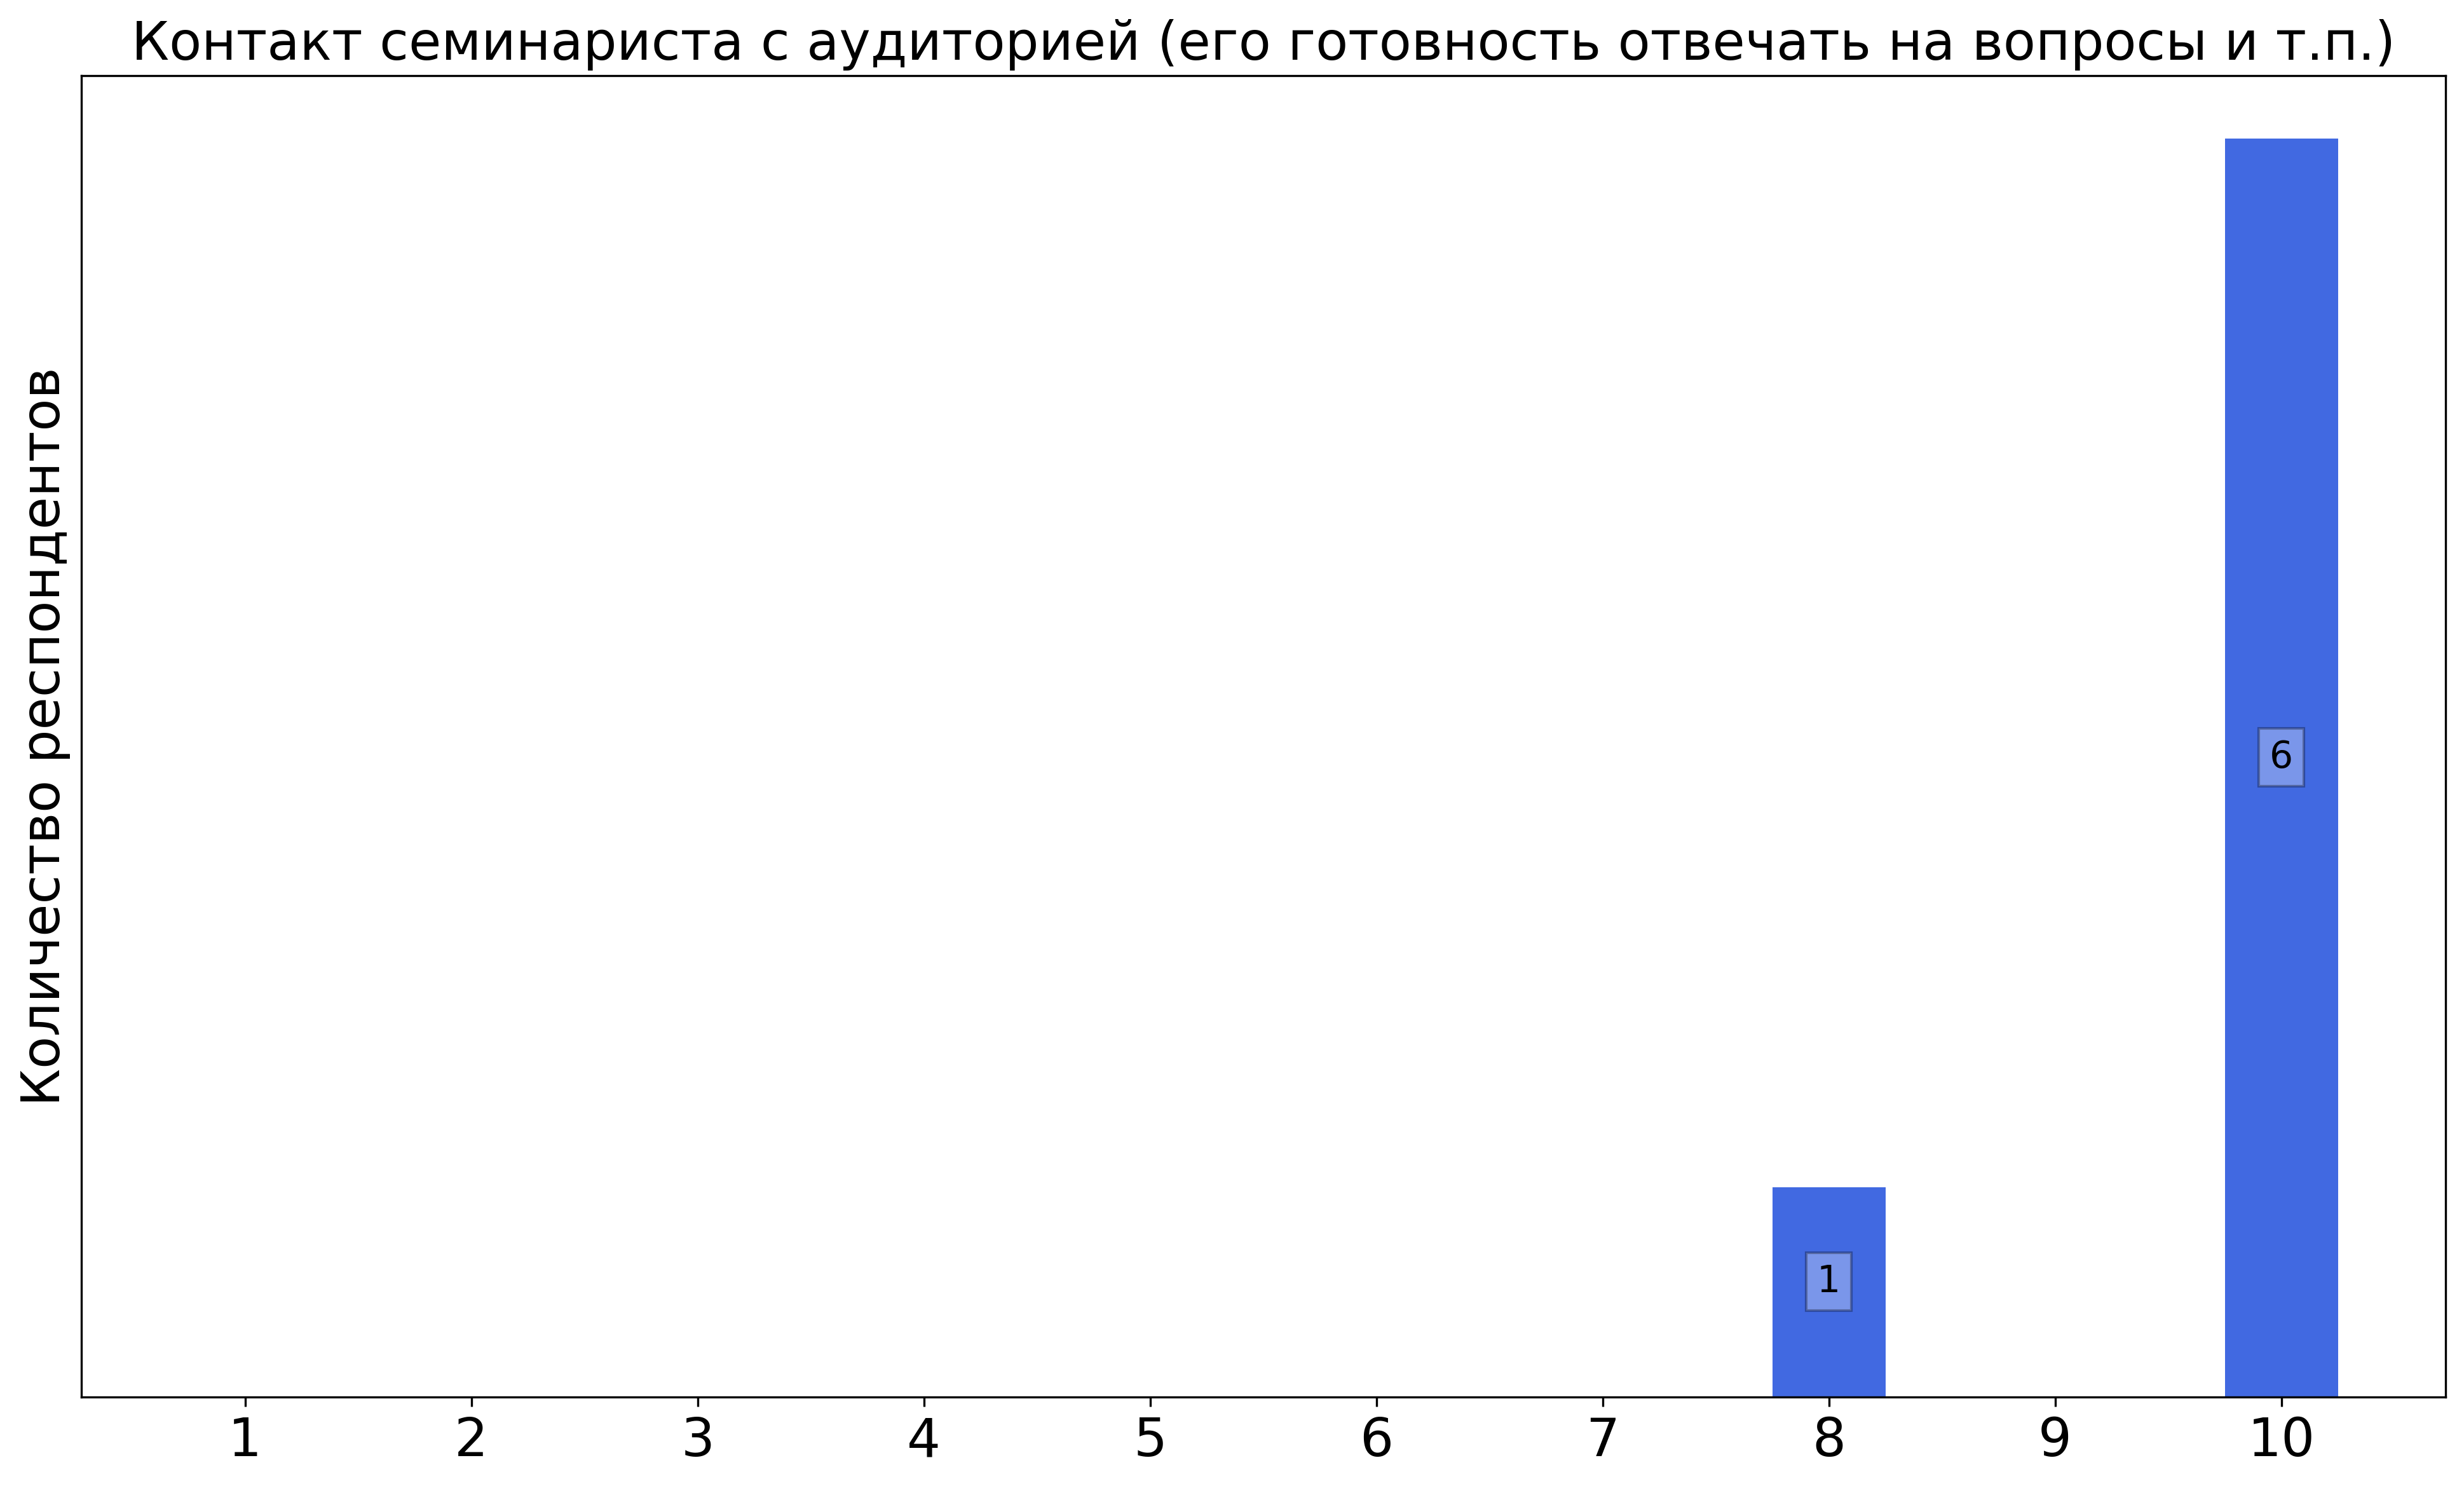
\includegraphics[width=\textwidth]{images/2 course/Кратные интегралы и теория поля/seminarists-marks-Петрович А.Ю.-0.png}
			\end{subfigure}
			\begin{subfigure}[b]{0.45\textwidth}
				\centering
				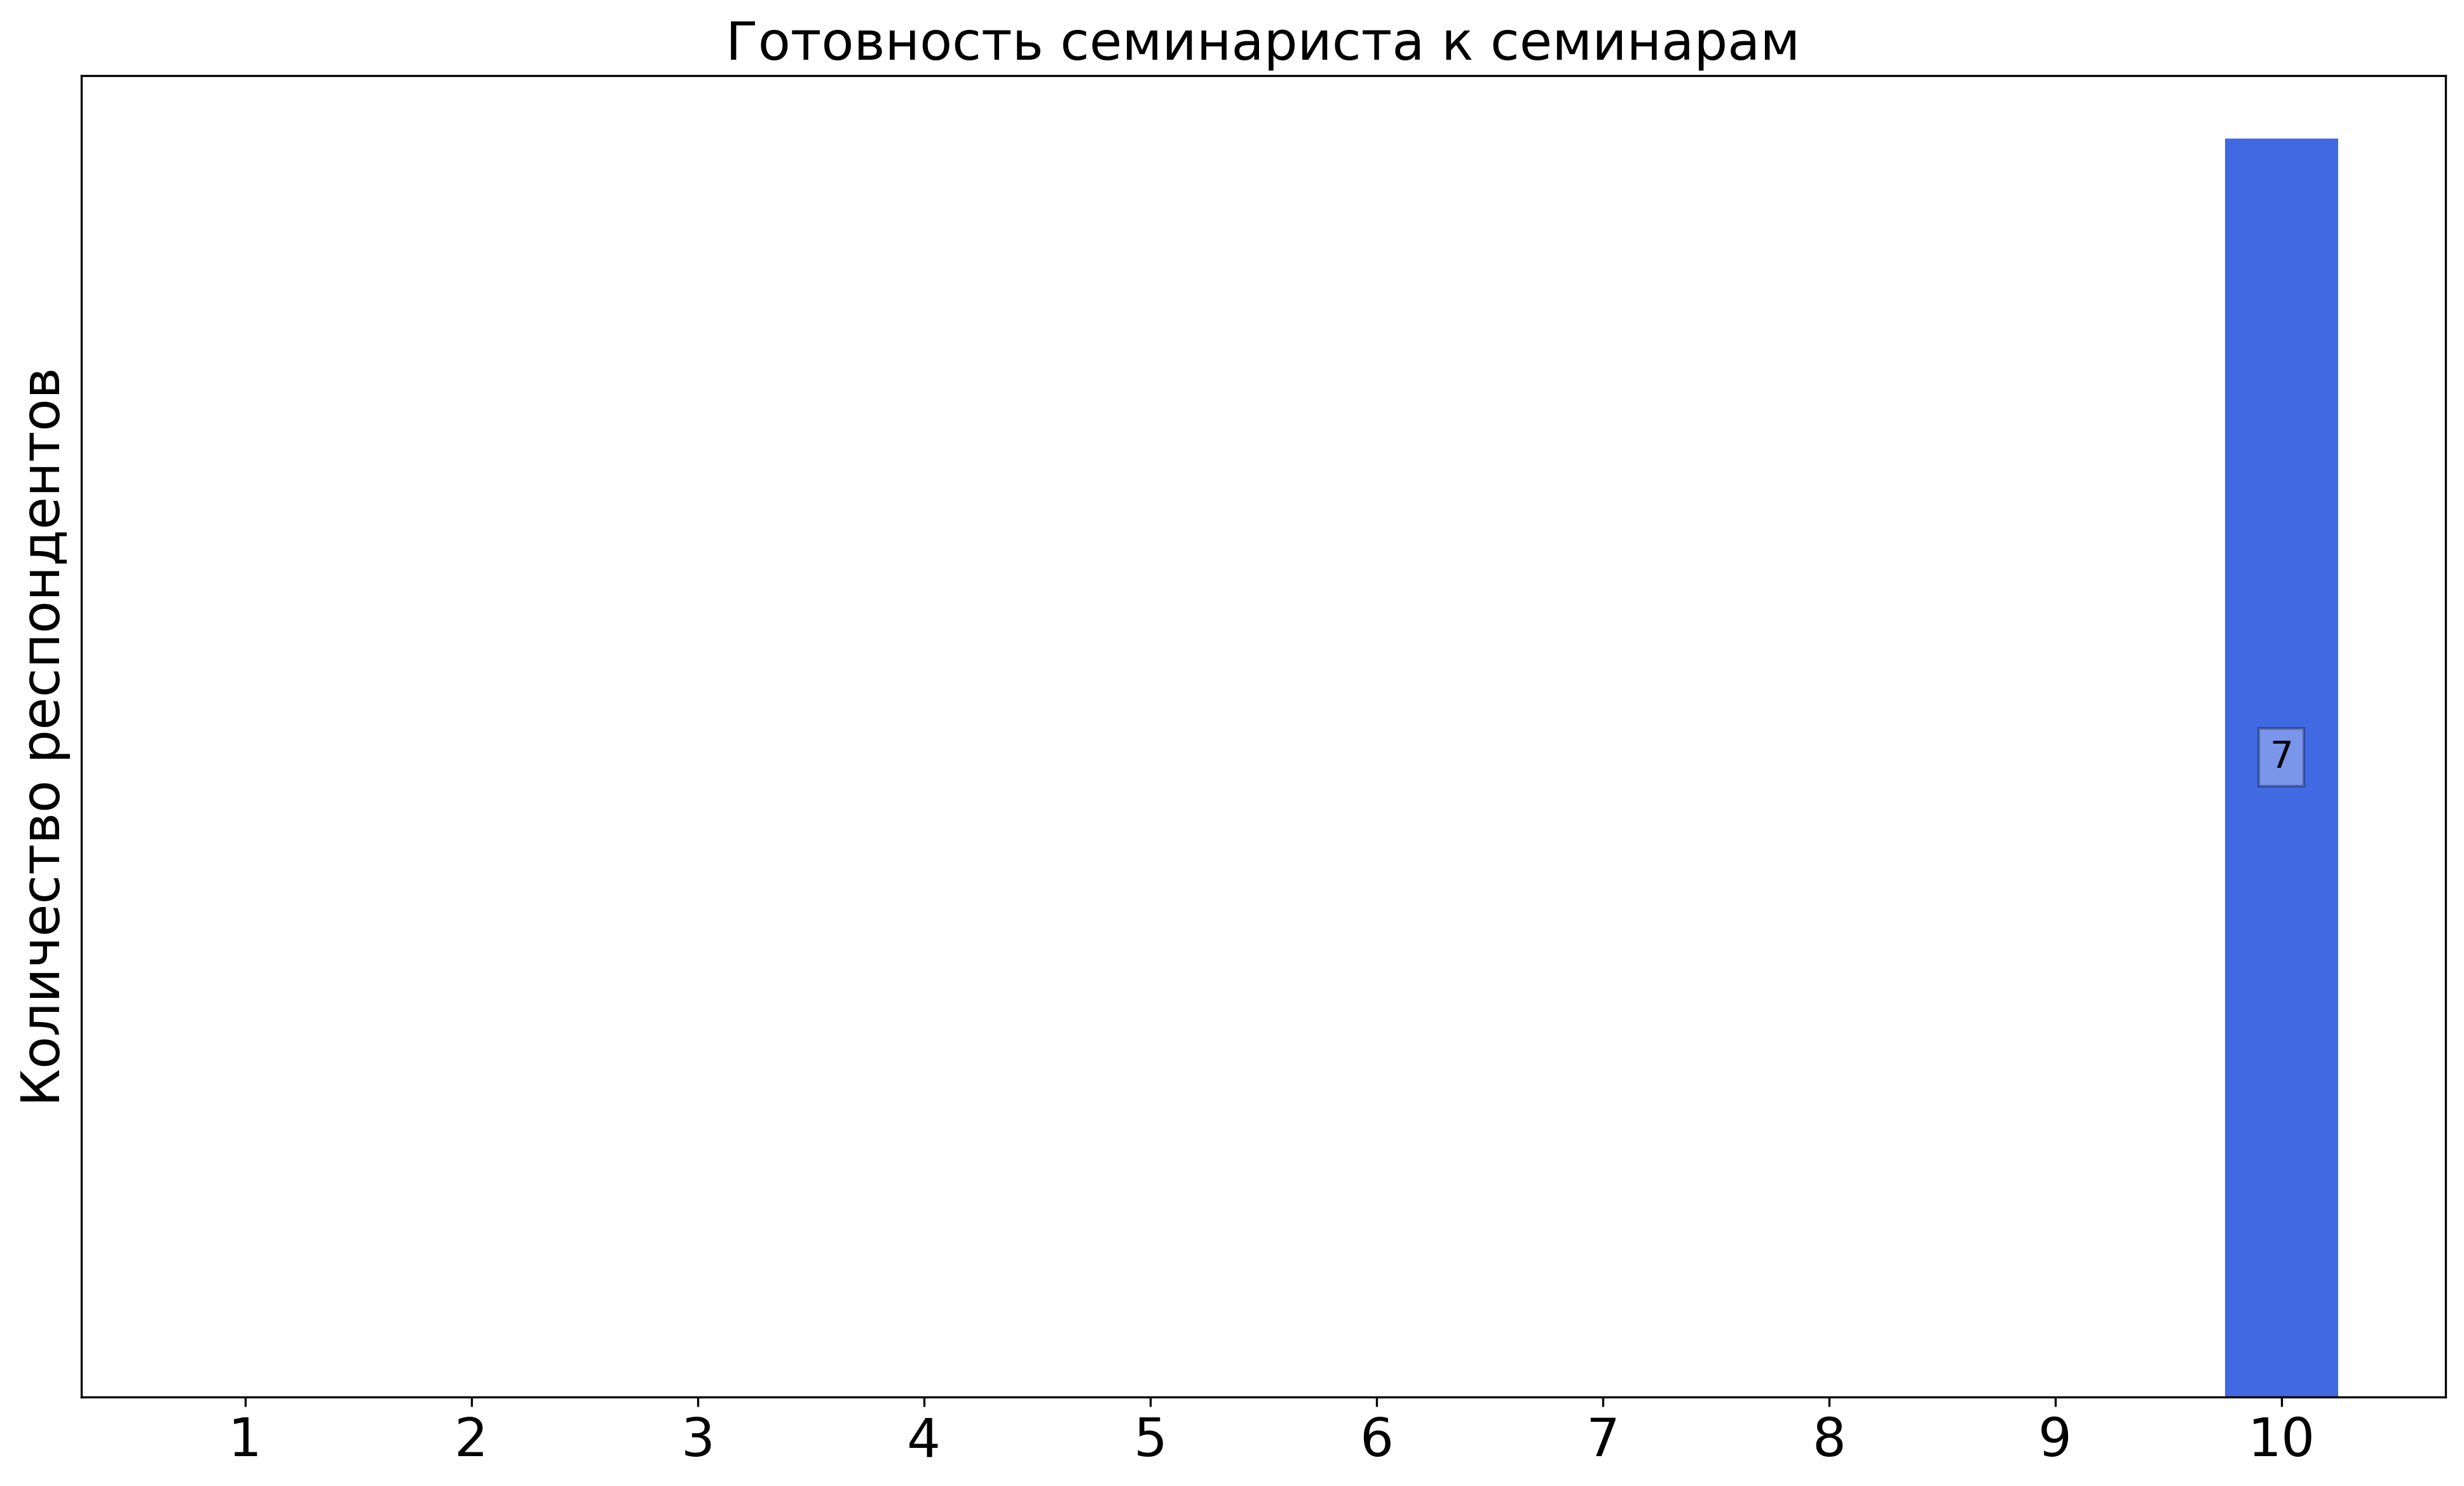
\includegraphics[width=\textwidth]{images/2 course/Кратные интегралы и теория поля/seminarists-marks-Петрович А.Ю.-1.png}
			\end{subfigure}
			\begin{subfigure}[b]{0.45\textwidth}
				\centering
				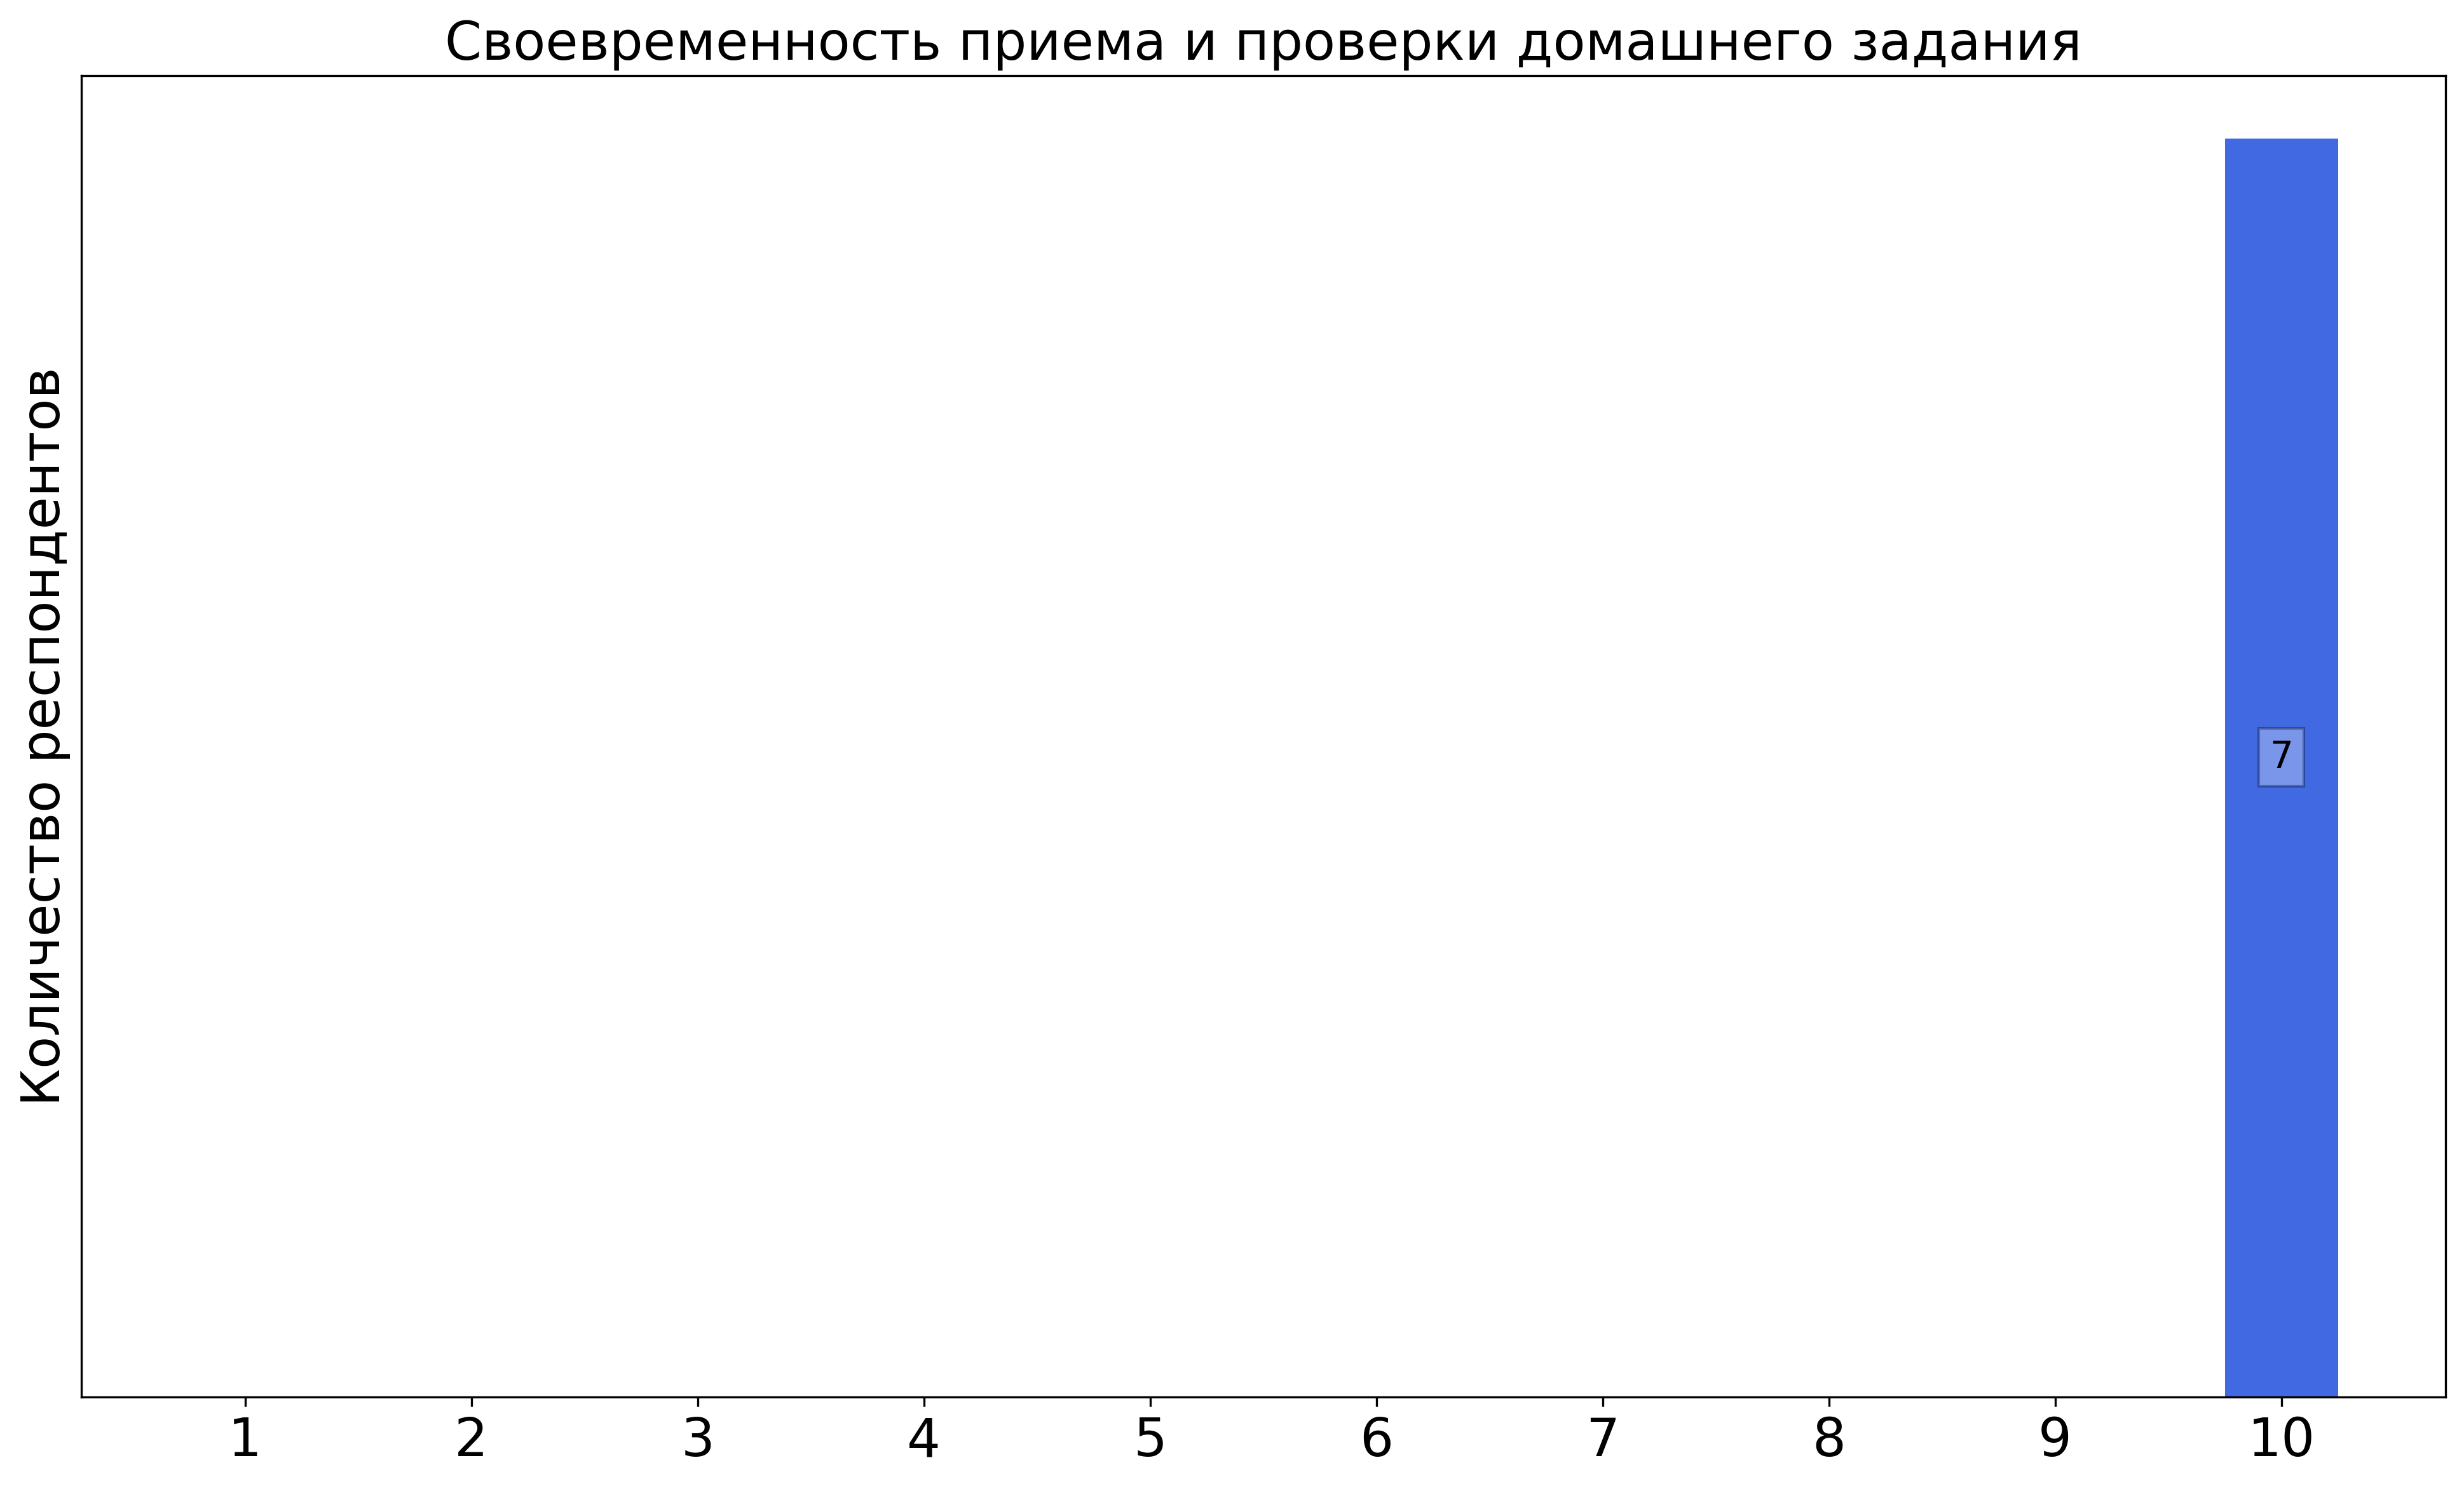
\includegraphics[width=\textwidth]{images/2 course/Кратные интегралы и теория поля/seminarists-marks-Петрович А.Ю.-2.png}
			\end{subfigure}
			\begin{subfigure}[b]{0.45\textwidth}
				\centering
				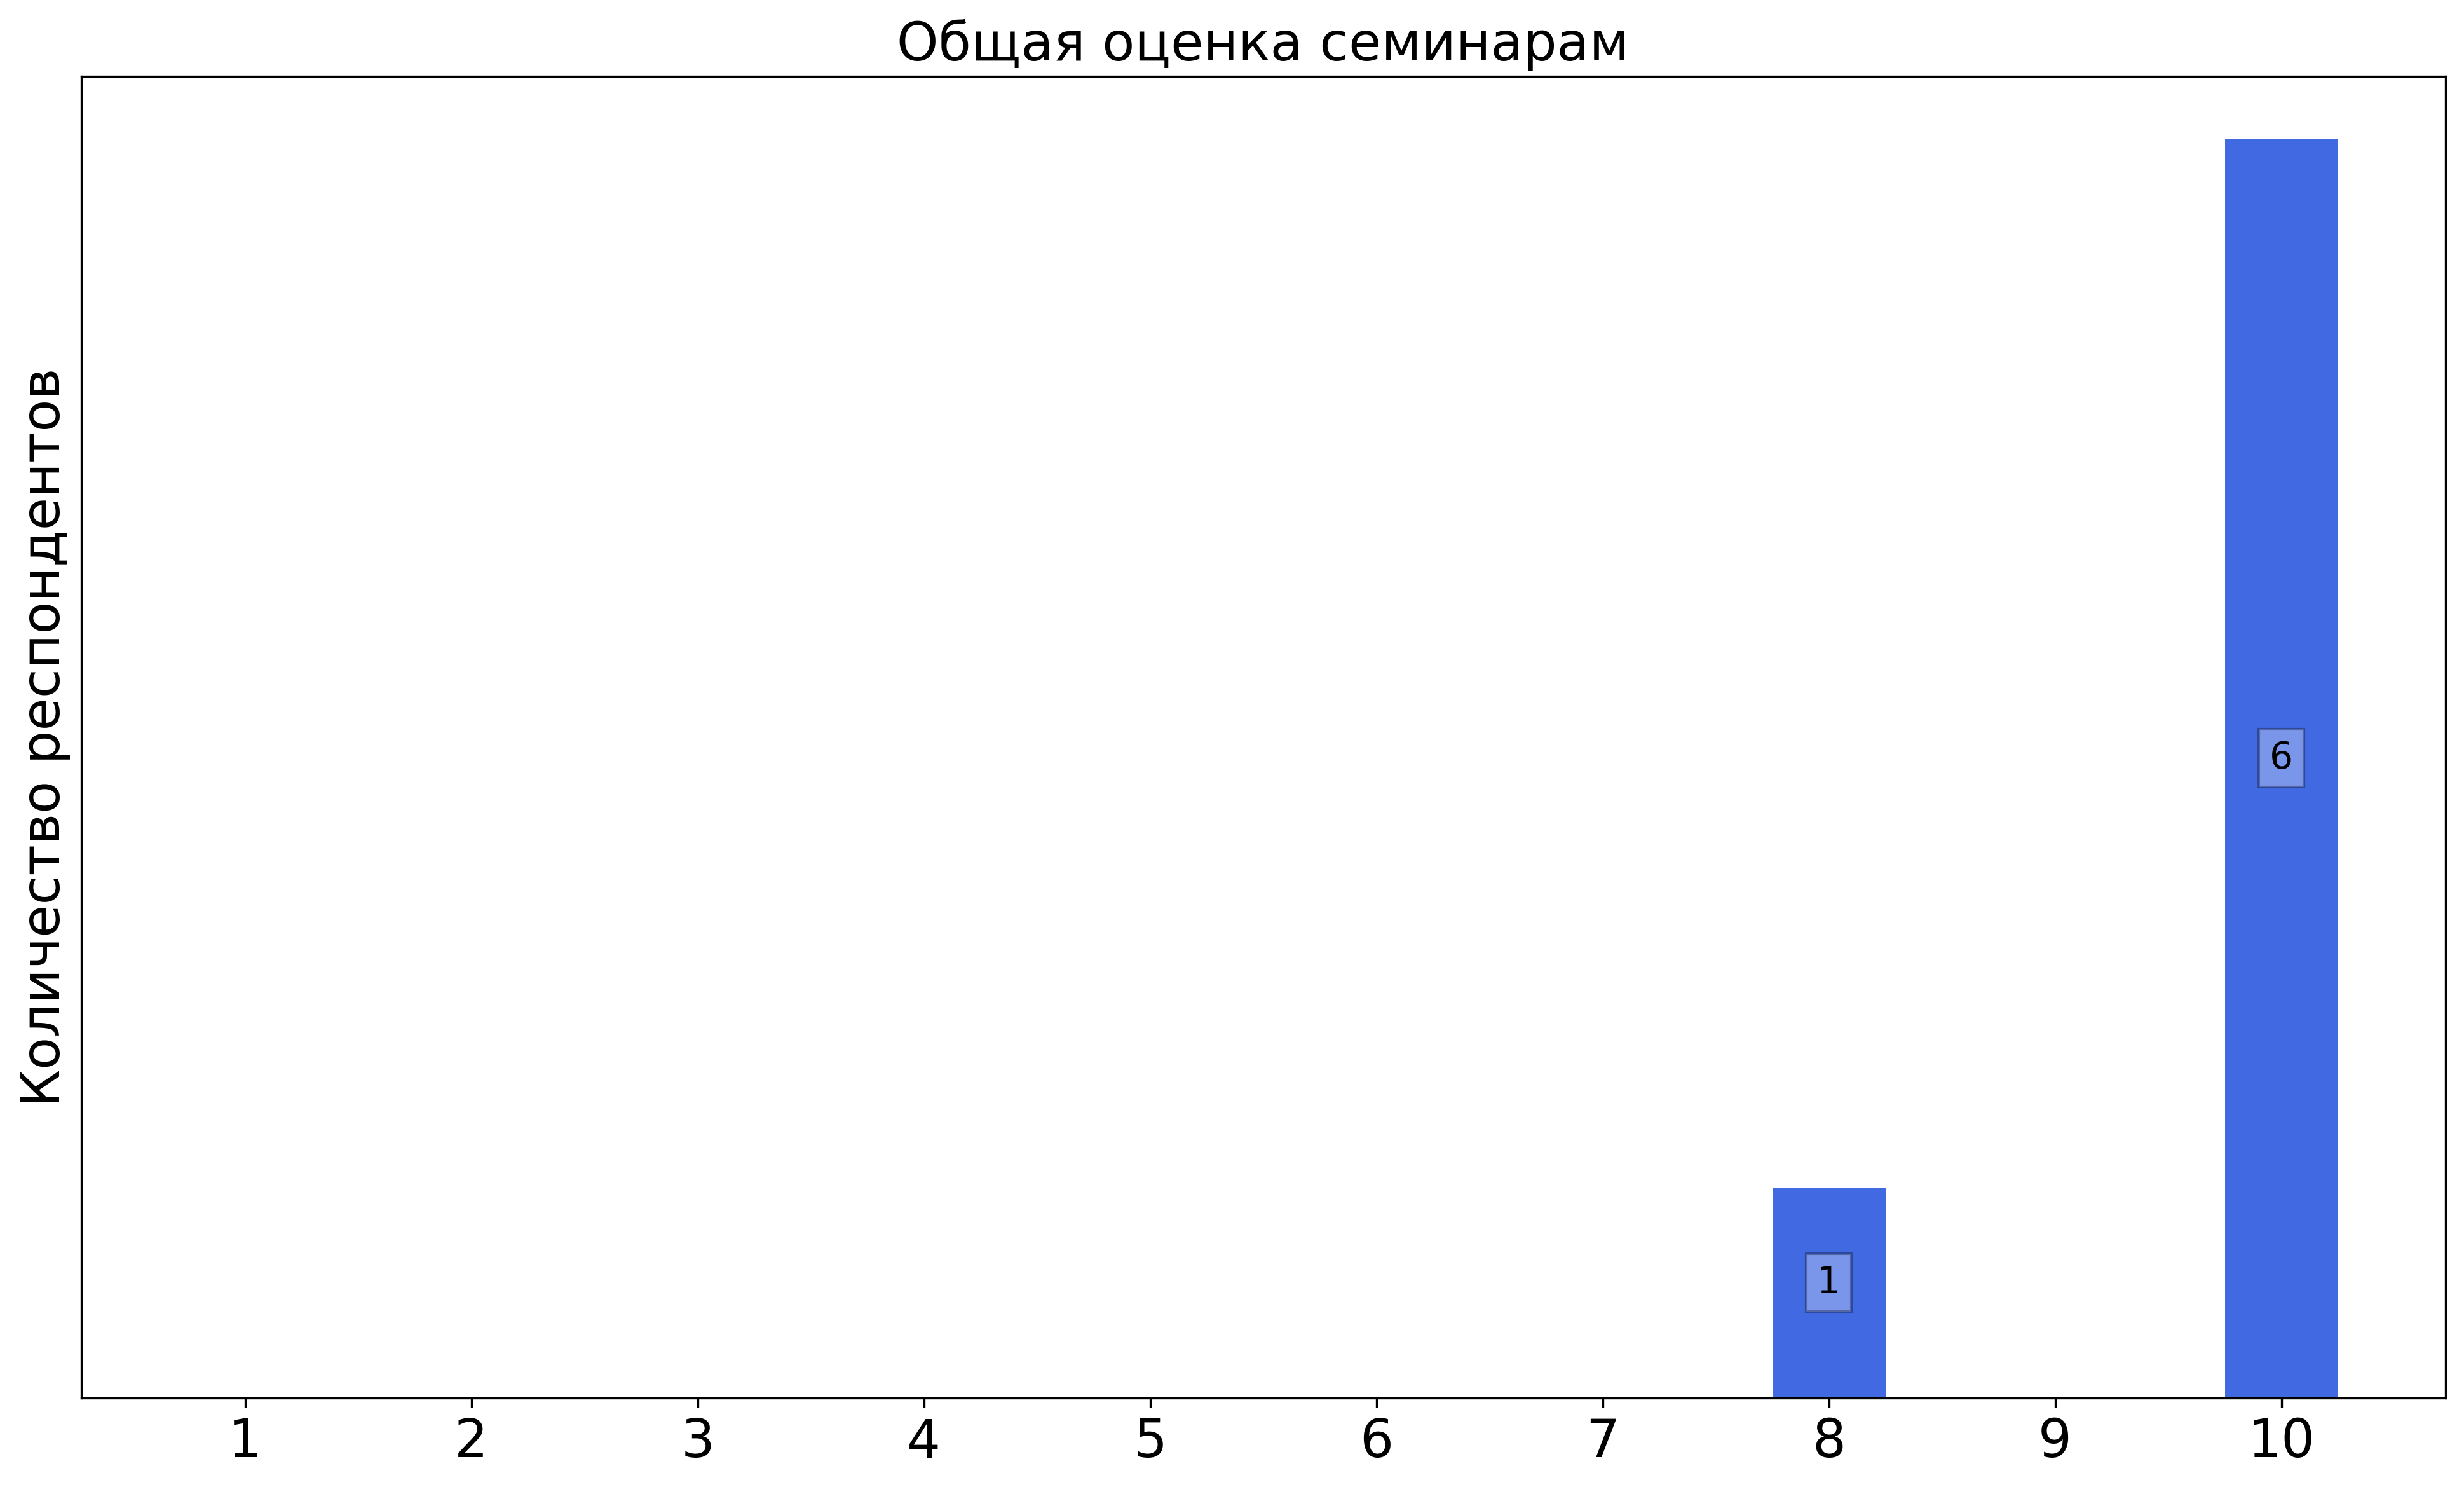
\includegraphics[width=\textwidth]{images/2 course/Кратные интегралы и теория поля/seminarists-marks-Петрович А.Ю.-3.png}
			\end{subfigure}	
			\caption{Оценки респондентов о качестве преподавания семинаров}
		\end{figure}

		\textbf{Комментарии студентов о семинаристе\protect\footnote{сохранены оригинальные орфография и пунктуация}}
            \begin{commentbox} 
                Петрович супер семинарист 10/10 
            \end{commentbox} 
        
            \begin{commentbox} 
                Хорошие семинары 
            \end{commentbox}

        
    \subsubsection{Отзыв студентов о семинарах. Семинарист: Черняев А.В.}
        \begin{figure}[H]
            \centering
            \begin{subfigure}[b]{0.45\textwidth}
                \centering
                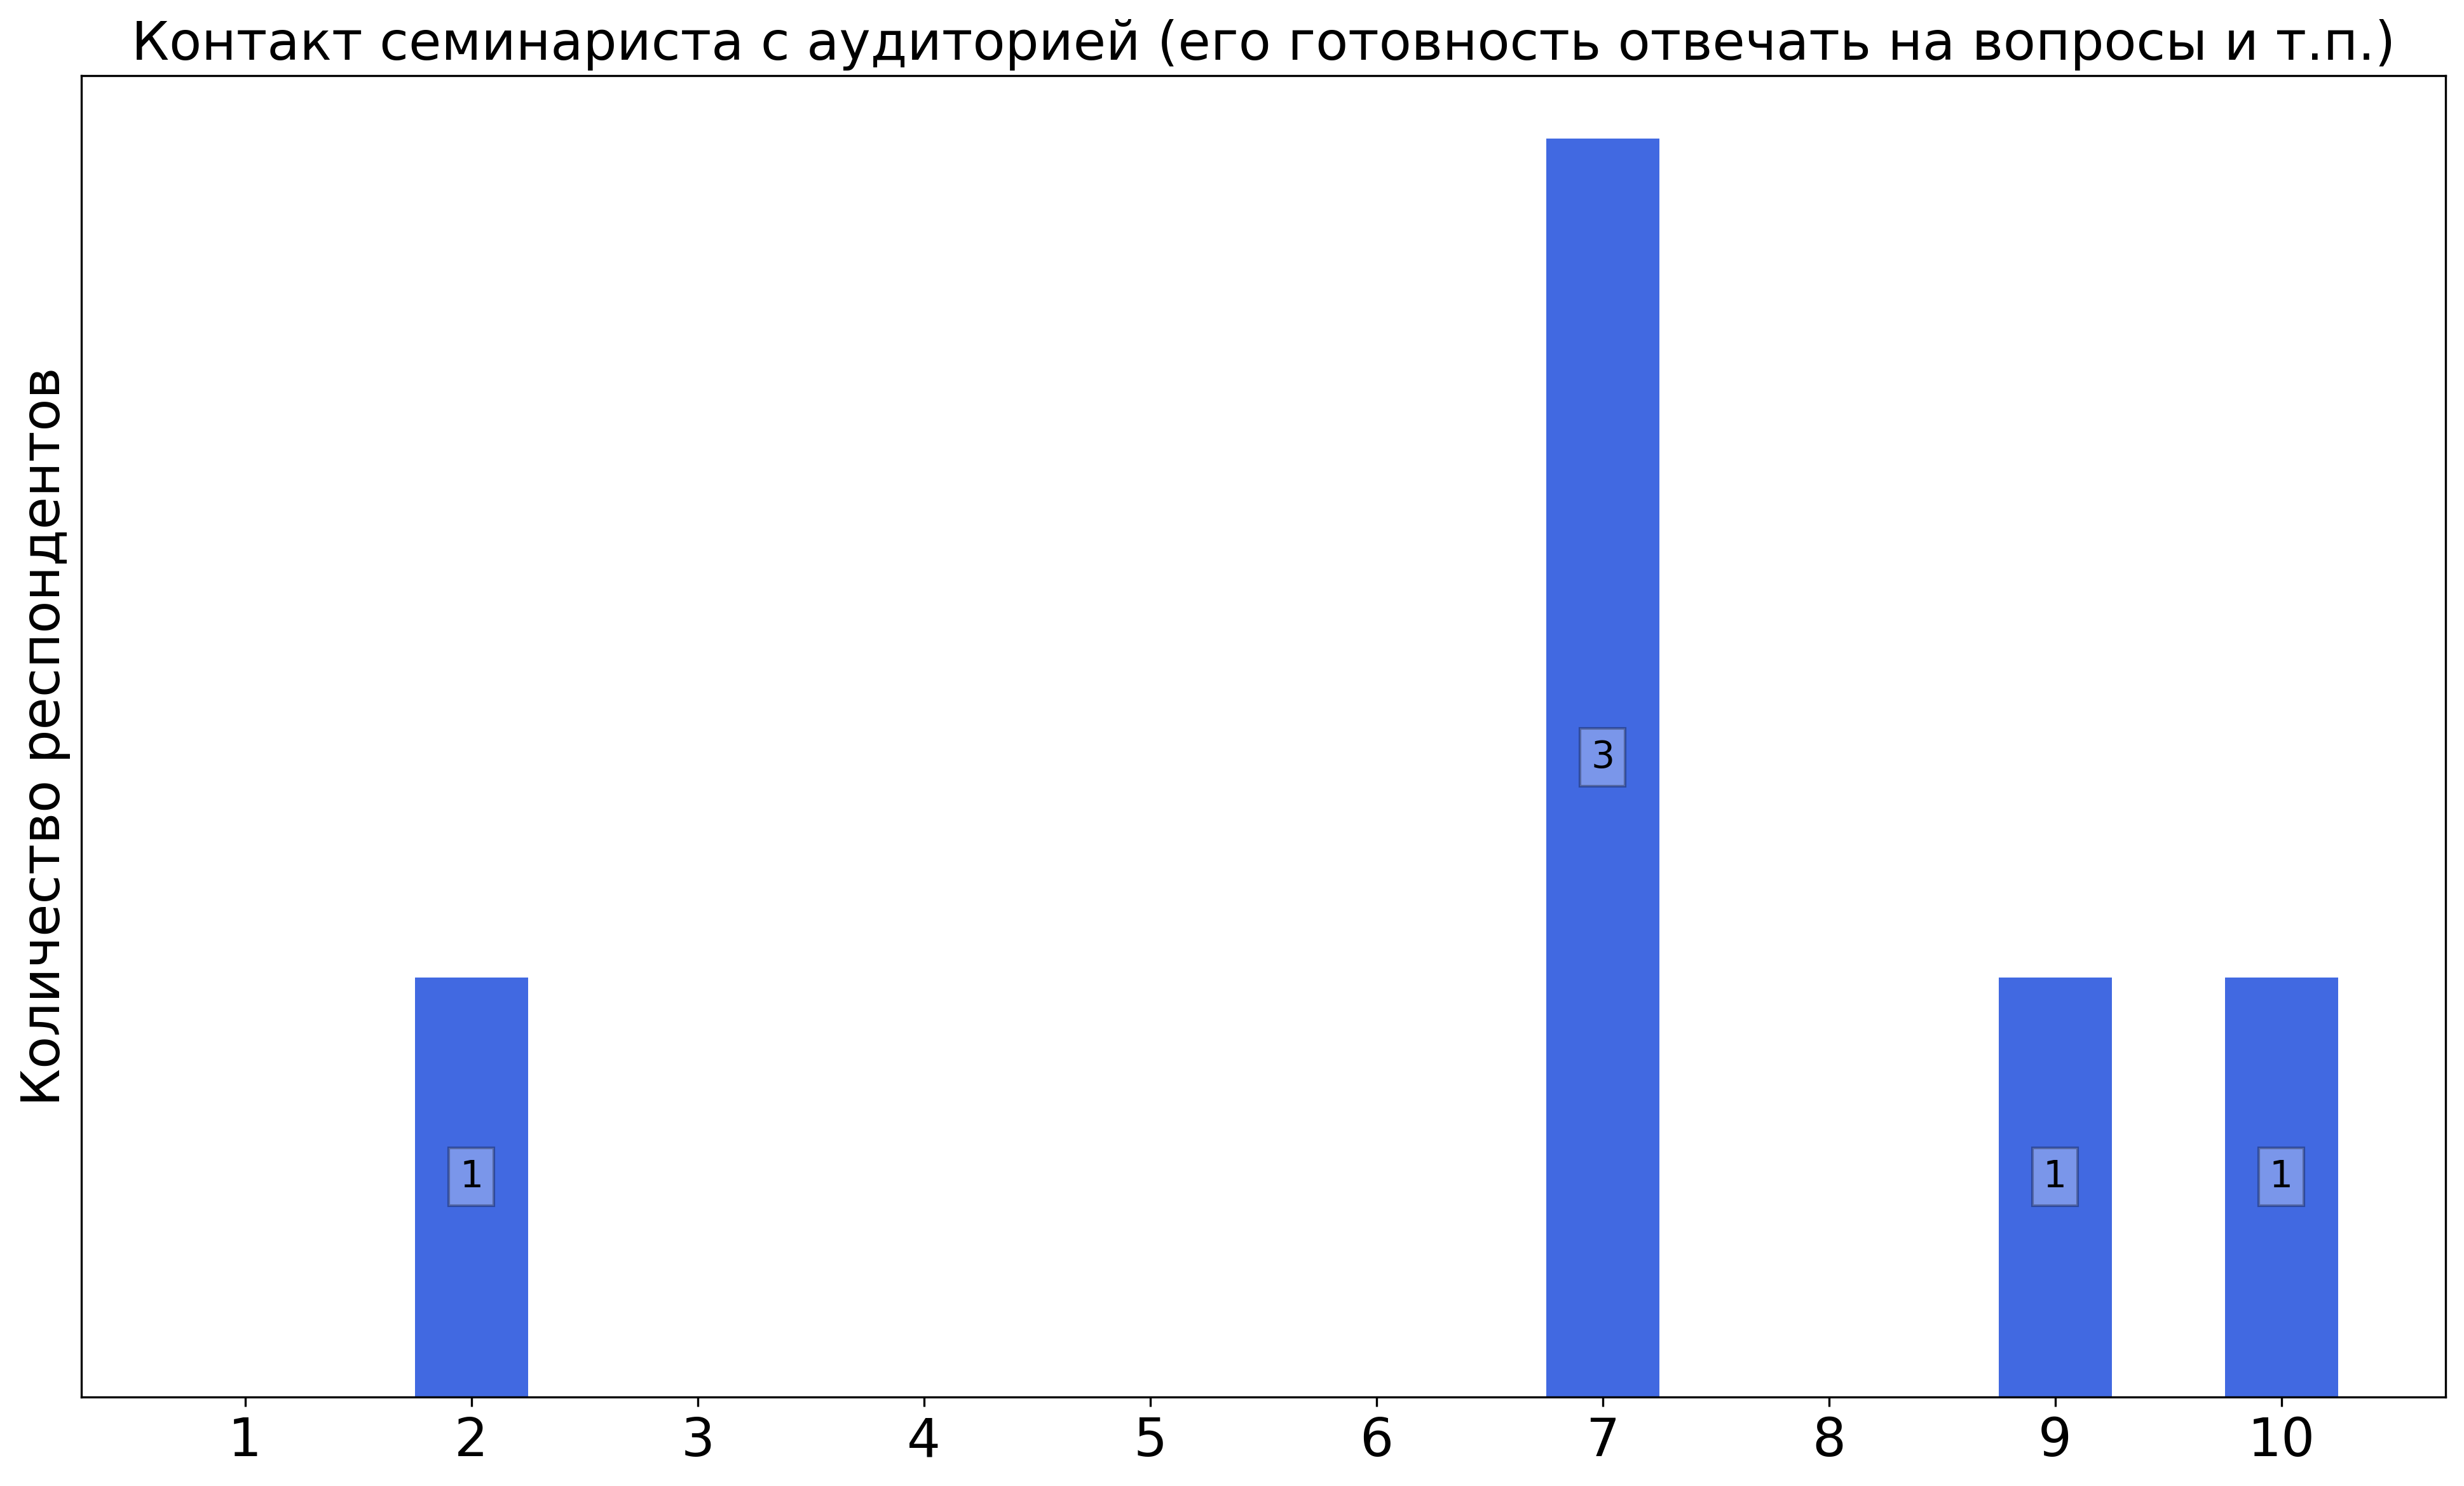
\includegraphics[width=\textwidth]{images/2 course/Кратные интегралы и теория поля/seminarists-marks-Черняев А.В.-0.png}
            \end{subfigure}
            \begin{subfigure}[b]{0.45\textwidth}
                \centering
                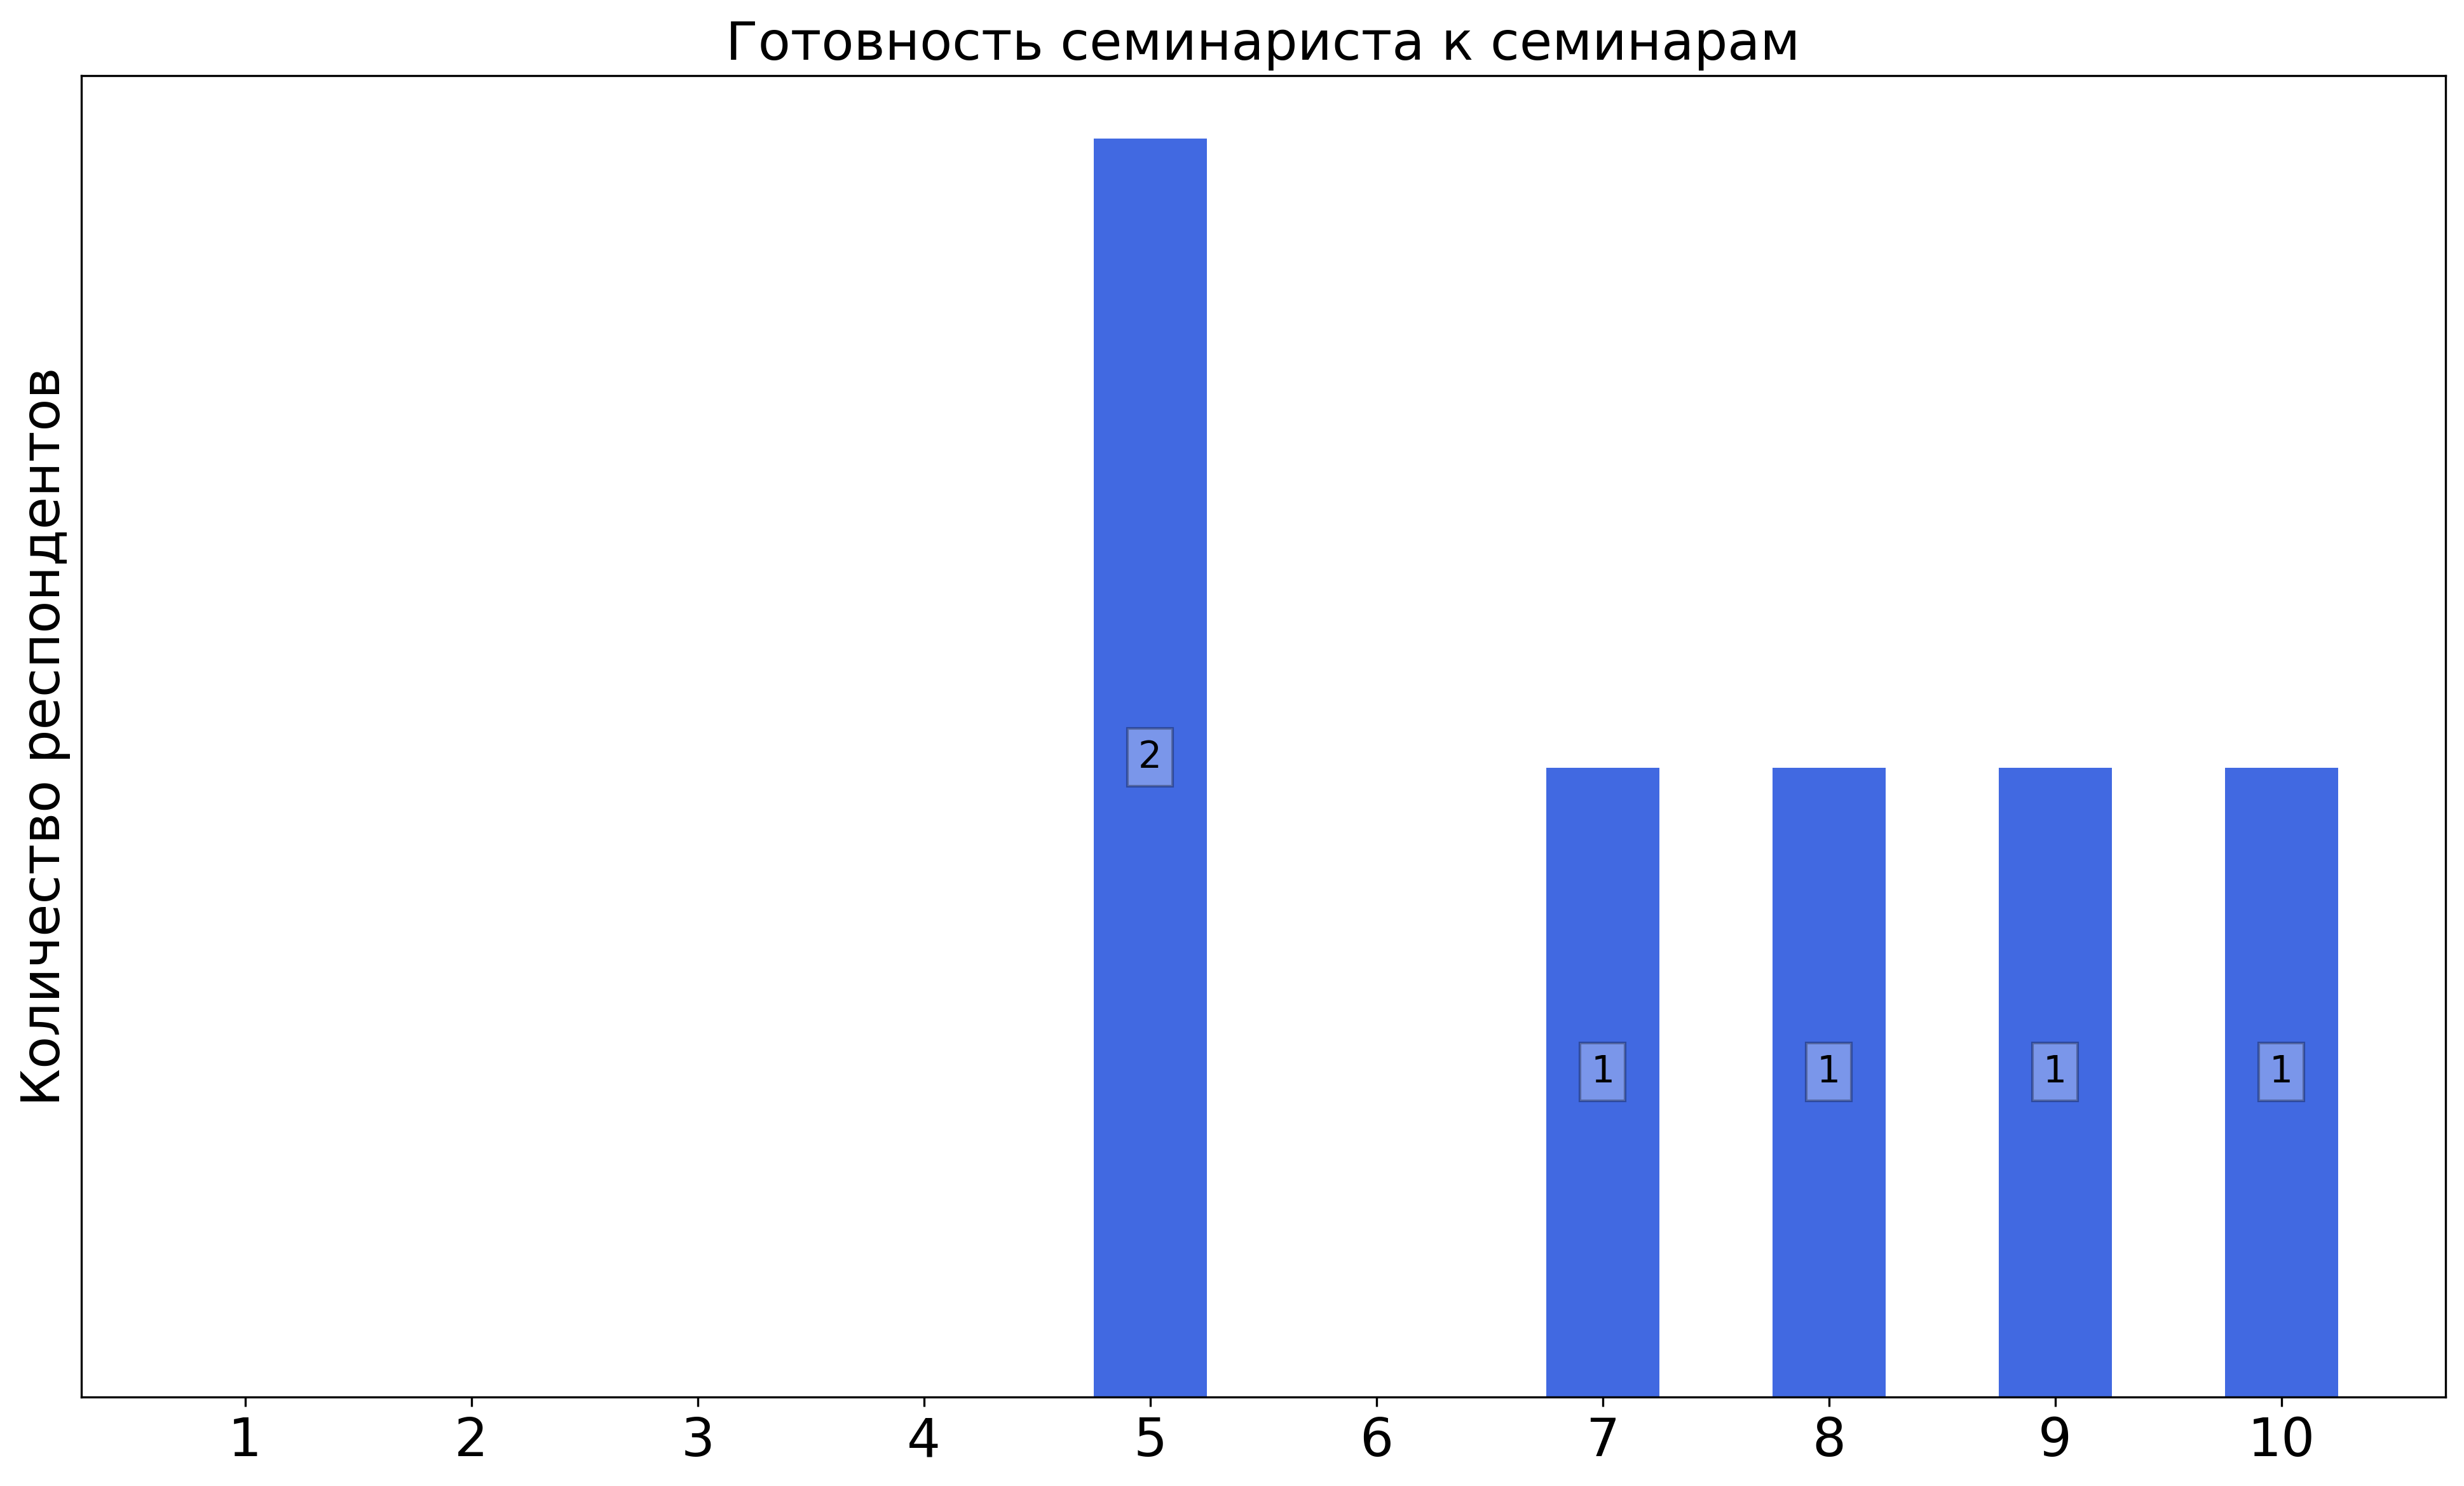
\includegraphics[width=\textwidth]{images/2 course/Кратные интегралы и теория поля/seminarists-marks-Черняев А.В.-1.png}
            \end{subfigure}
            \begin{subfigure}[b]{0.45\textwidth}
                \centering
                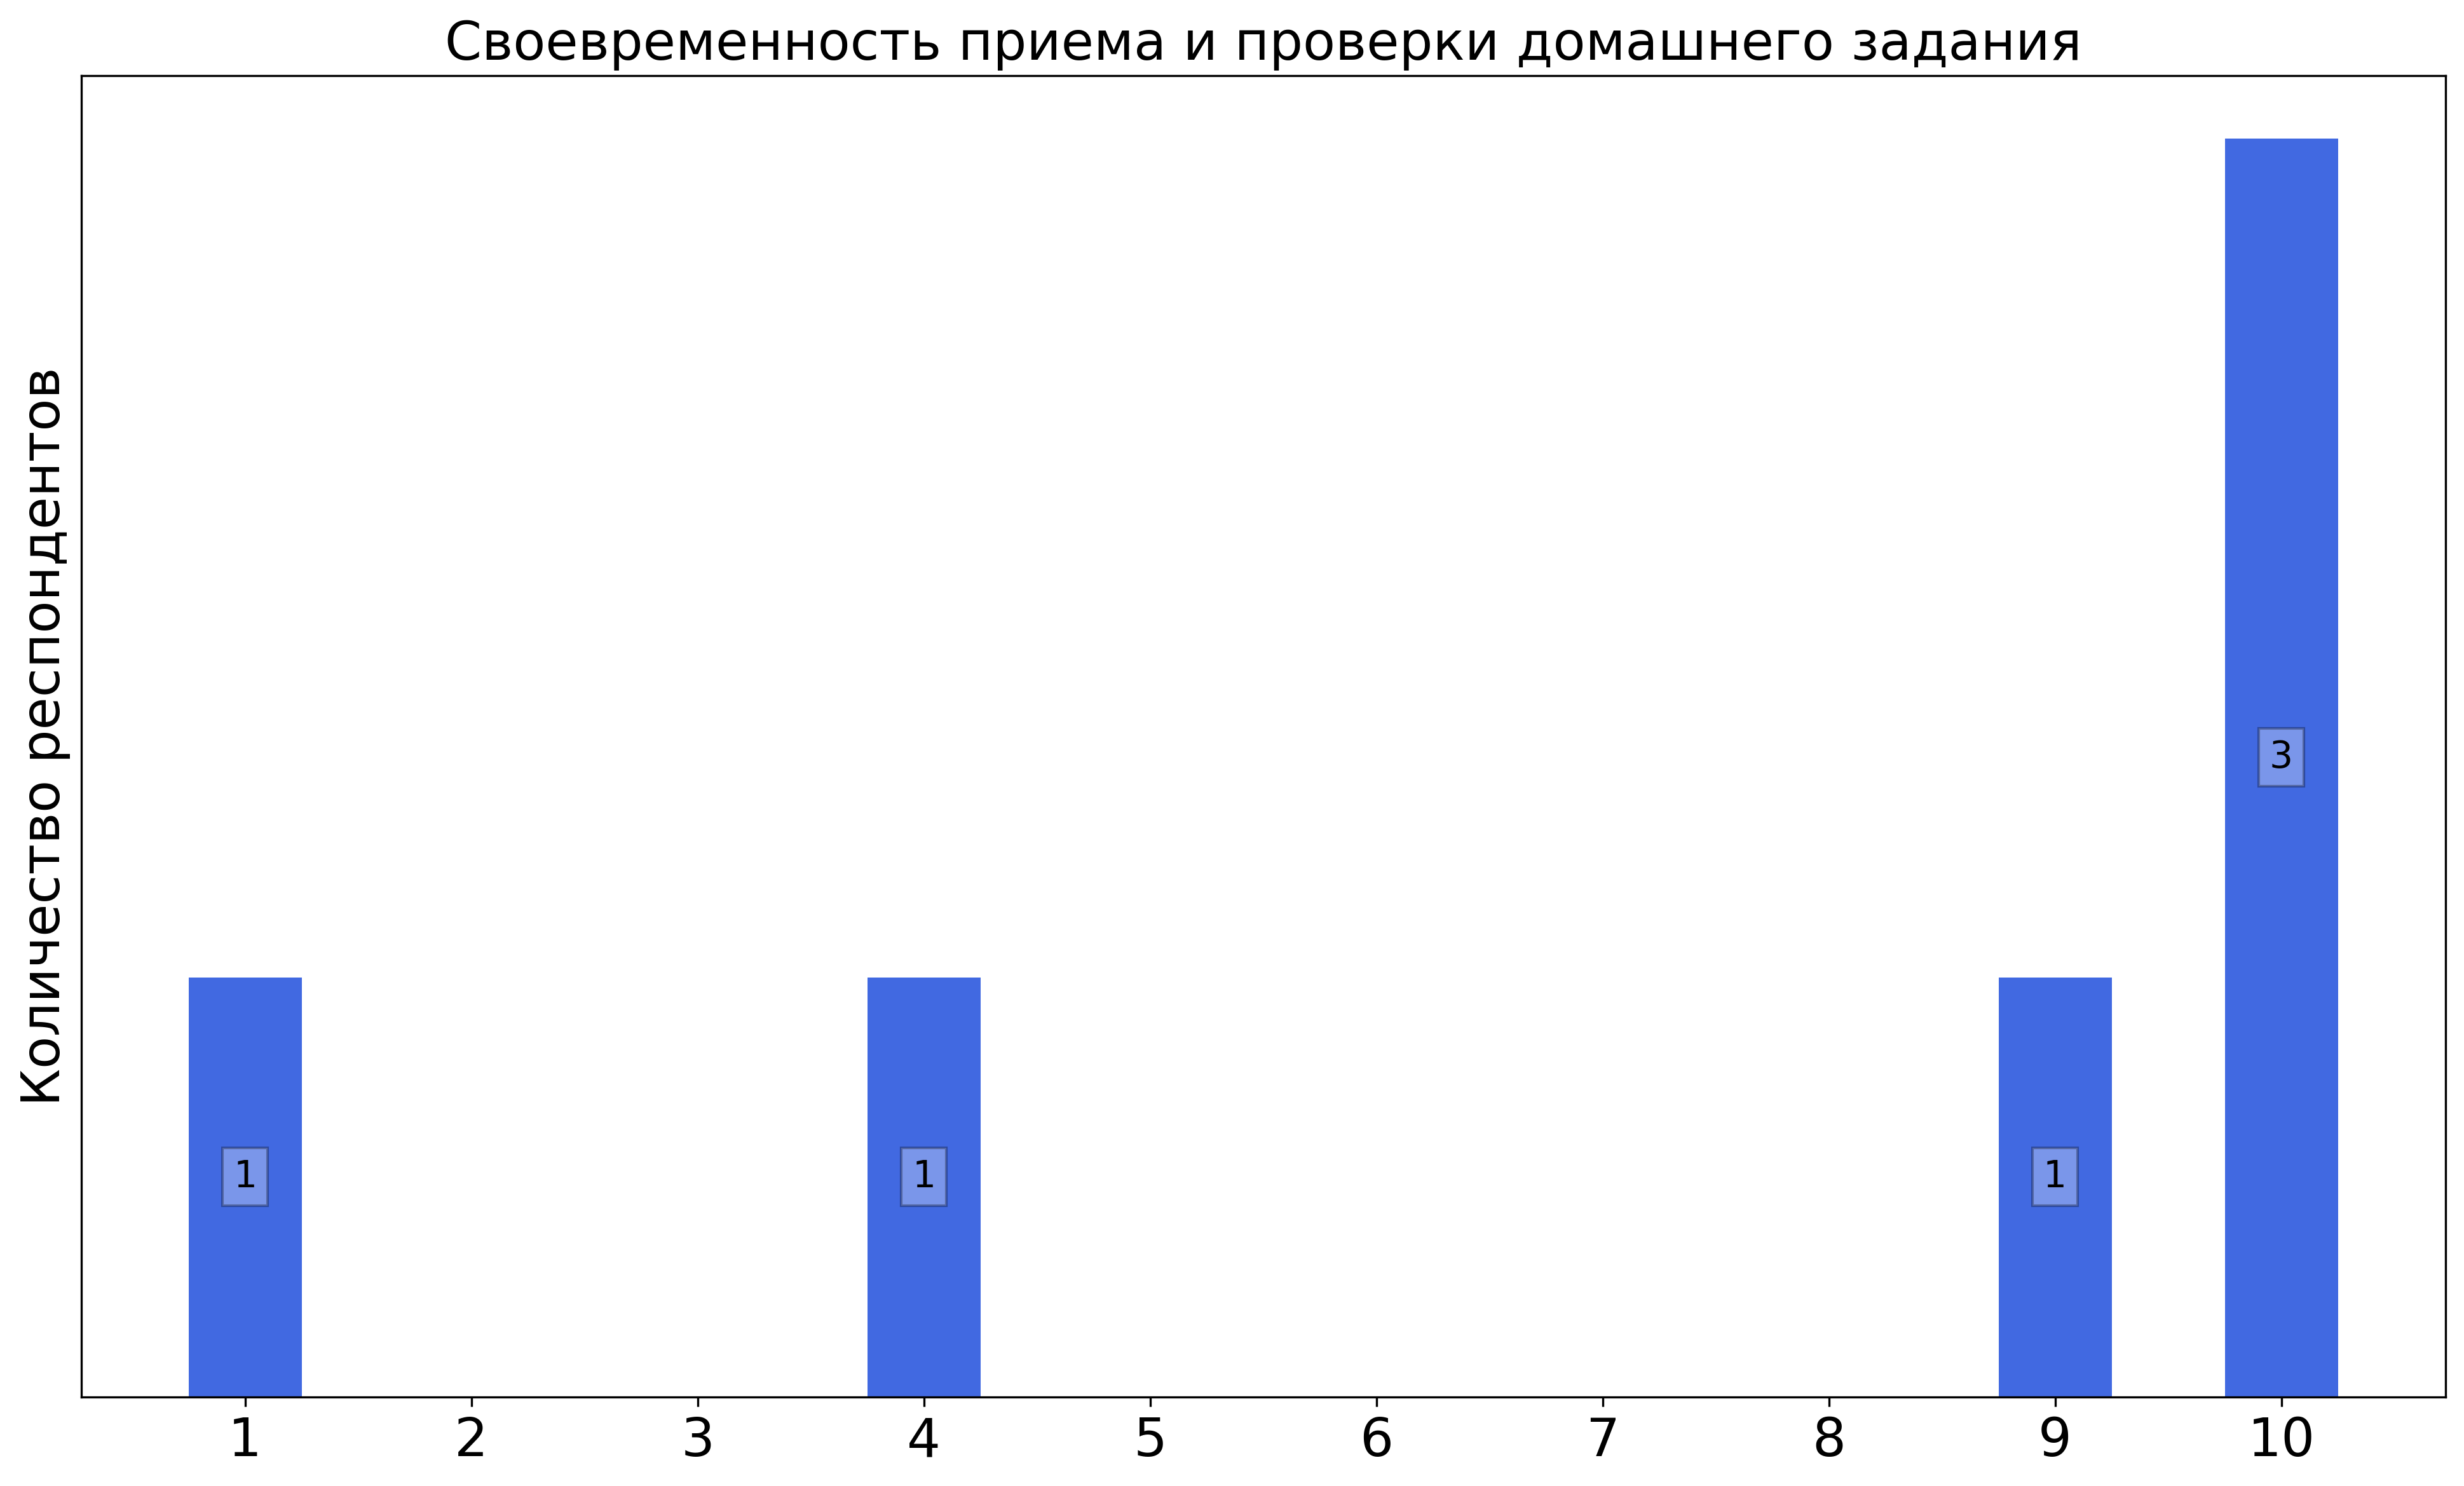
\includegraphics[width=\textwidth]{images/2 course/Кратные интегралы и теория поля/seminarists-marks-Черняев А.В.-2.png}
            \end{subfigure}
            \begin{subfigure}[b]{0.45\textwidth}
                \centering
                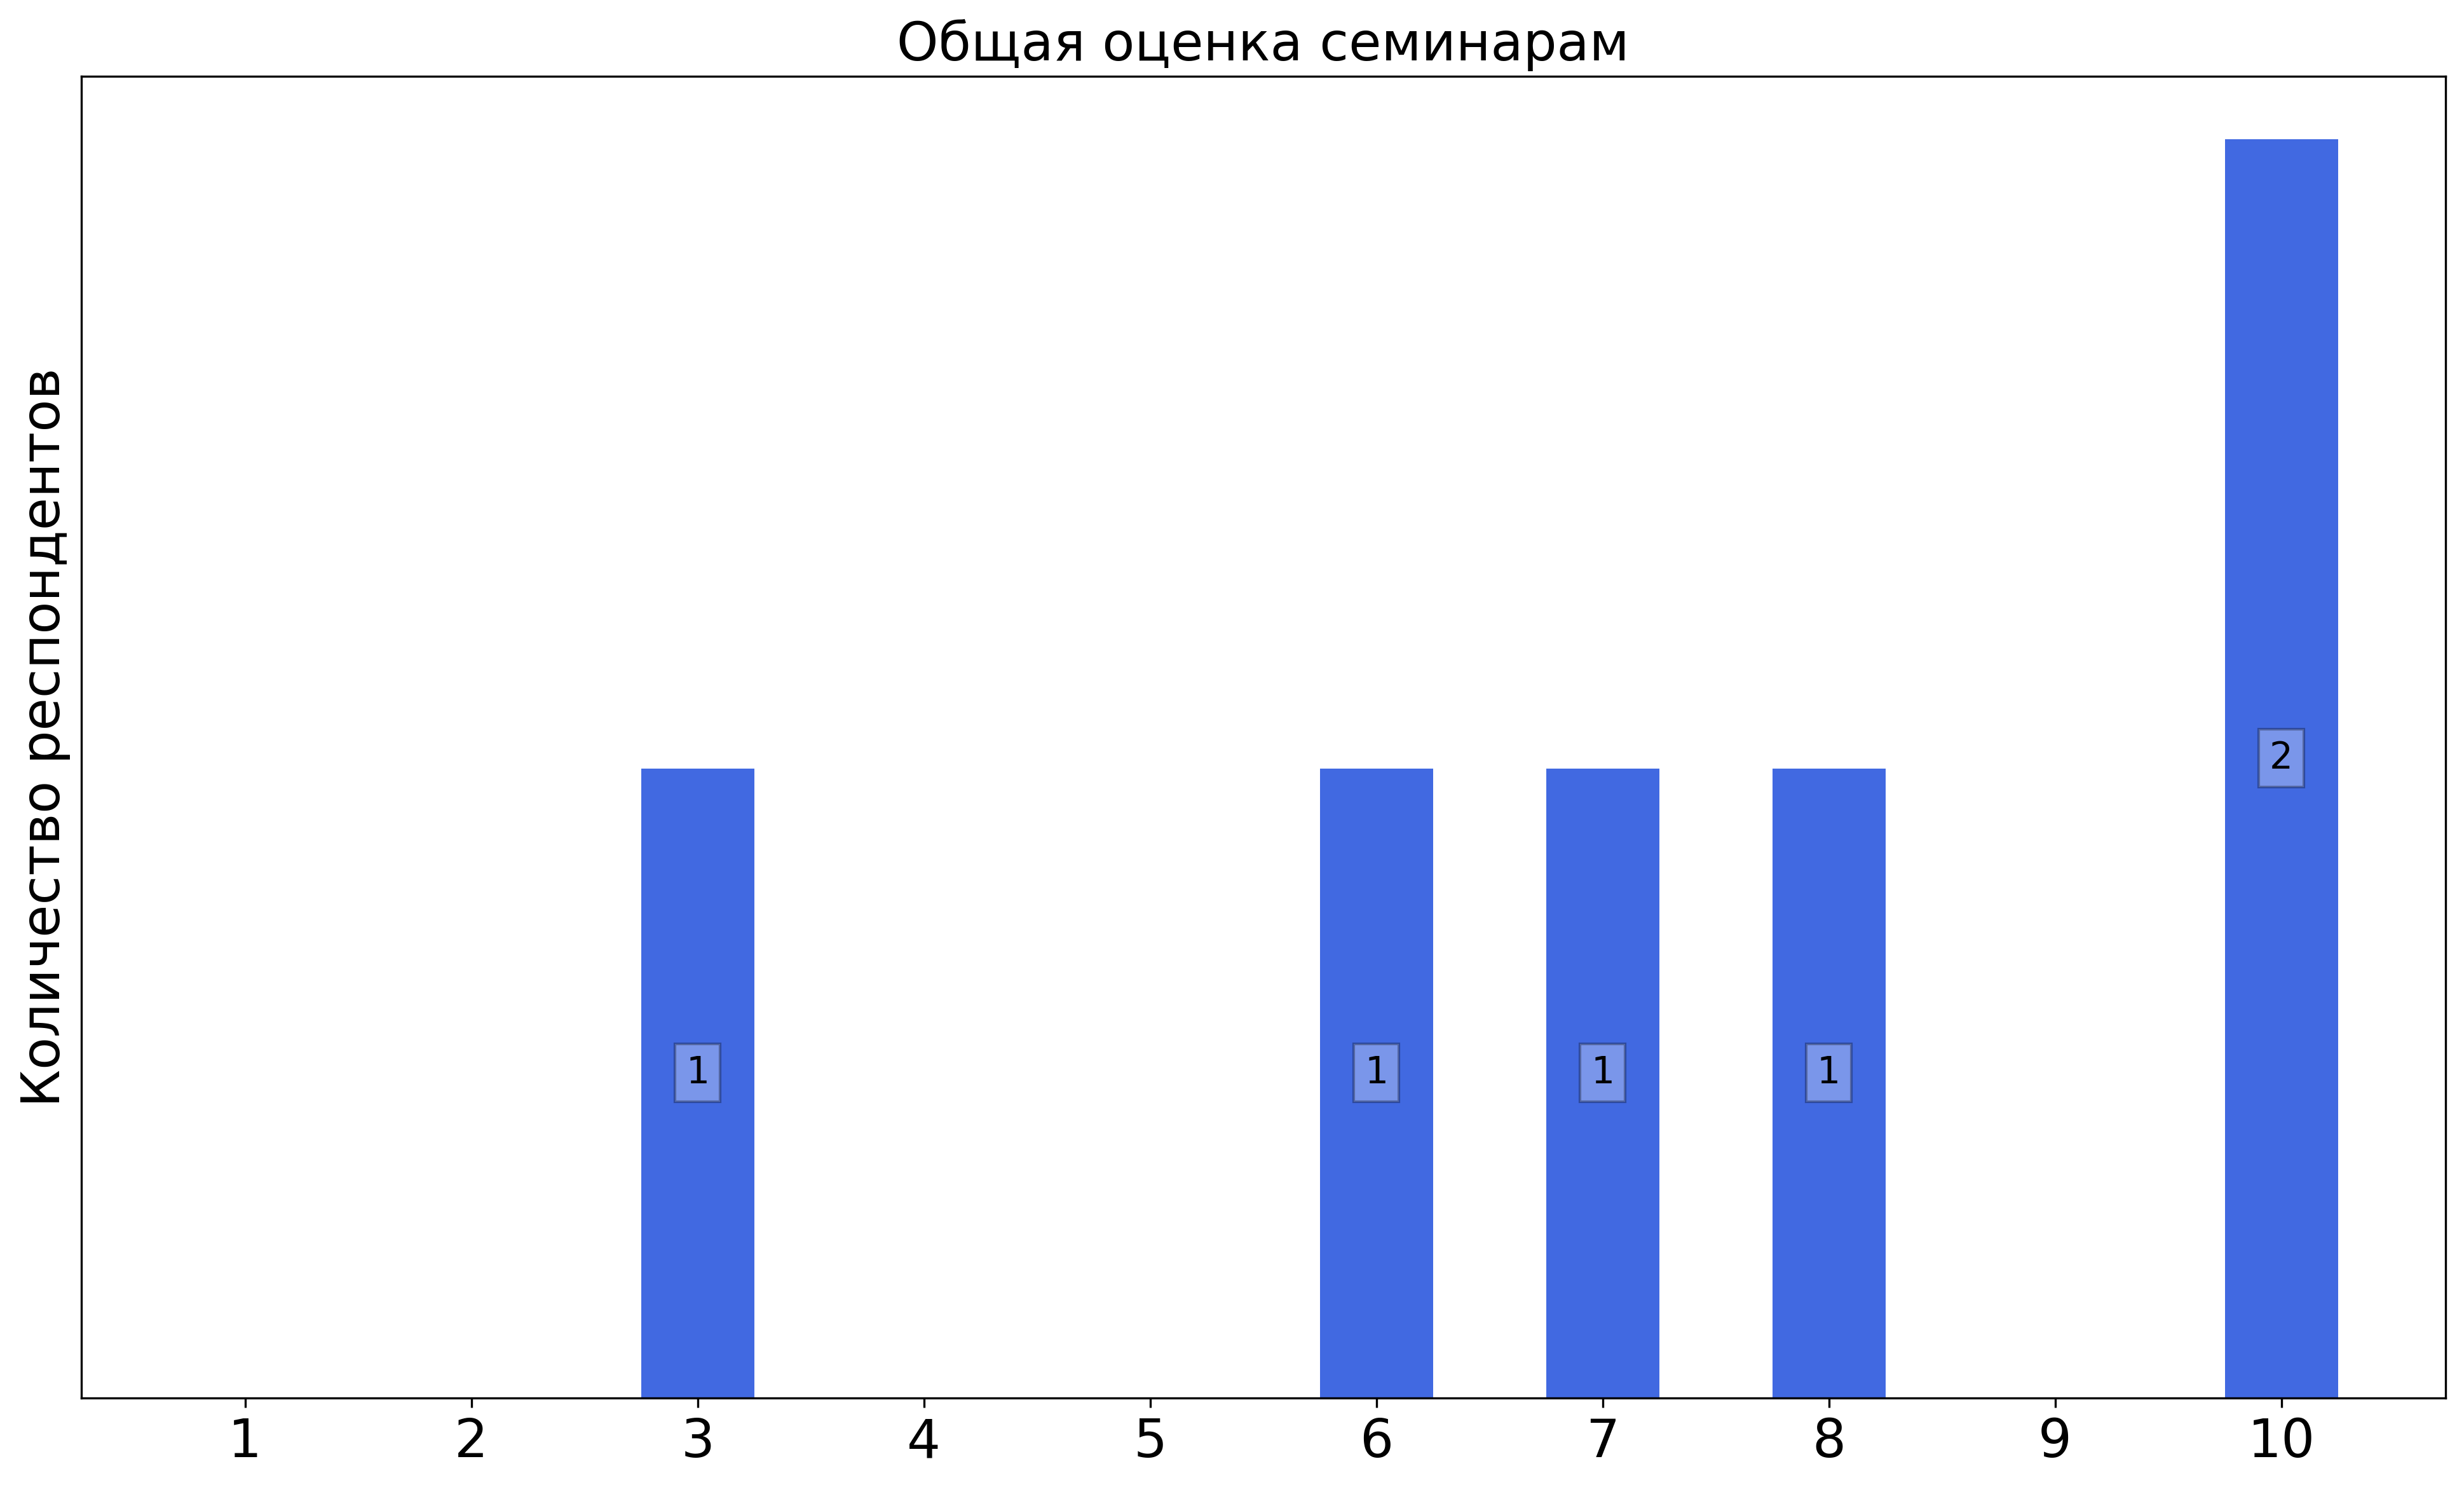
\includegraphics[width=\textwidth]{images/2 course/Кратные интегралы и теория поля/seminarists-marks-Черняев А.В.-3.png}
            \end{subfigure}	
            \caption{Оценки респондентов о качестве преподавания семинаров}
        \end{figure}

        \textbf{Комментарии студентов о семинаристе\protect\footnote{сохранены оригинальные орфография и пунктуация}}
            \begin{commentbox} 
                хороший преподаватель, однако специфические методы рассказывания решения задач. сложно переносить методы при решении дз 
            \end{commentbox} 
        
            \begin{commentbox} 
                Черняев А.П. вёл у меня семинары по кратным интеграл и теории поля. К сожалению, на его семинарах я ничему научиться не смог и был вынужден заниматься самостоятально 
                Черняев А.П. не разбирает теорию, не вдаётся в тонкости задачи, а зачастую просто записывает решение на доске
                Семинары Черняева А.П. проходят в очень медленном темпе, потому что на задачу он может потратить половину пары, поэтому в конце семестра было отставание от программы
                Домашние задания Черняев А.П. считает нормальным проверять в последний день перед закрытием ведомостей и ставить оценку ниже положенной, потому что он не сможет, а скорее всего, просто не захочет искать задачи и скажет, что их нет 
            \end{commentbox} 
        

    \subsubsection{Прочие комментарии и предложения по улучшению курса}
        \begin{commentbox}
            Можно добавить для большего понимания некоторые прикладные задачи из курса общей физики
        \end{commentbox}